%--------------------
% Packages
% -------------------
\documentclass[11pt,a4paper]{article}
\usepackage[utf8x]{inputenc}
\usepackage[T1]{fontenc}
%\usepackage{gentium}
\usepackage{mathptmx} % Use Times Font
\newcommand{\heading}[1]{\vspace{1em}\noindent\textbf{#1}\par\vspace{0.5em}}

%1. Choose a change request for the system.
%2. Perform impact analysis, define implementation alternatives, estimates.
%3. Define a project plan for implementing the change.
%4. Elaborate the requirements using the ICONIX process.
%   The expected output: Change request and its impact analysis document, project
%   plan document and the requirements document.
%
%Suggested requirements document structure:
%1. Context. Context of the system and the planned change, etc.
%2. Static Model. As defined in the ICONIX process, up to the robustness analysis.
%3. Use Cases. Behavioural description, as defined in the ICONIX process, up to the robustness analysis.
%4. Traceability. Mapping with requirements as well as between the views.
%This document only covers the parts of the model, that are necessary to describe the requirements in question.


\usepackage{comment}
\usepackage[pdftex]{graphicx} % Required for including pictures
\usepackage[pdftex,linkcolor=black,pdfborder={0 0 0}]{hyperref} % Format links for pdf
\usepackage{calc} % To reset the counter in the document after title page
\usepackage{enumitem} % Includes lists

\frenchspacing % No double spacing between sentences
\linespread{1.2} % Set linespace
\usepackage[a4paper, lmargin=0.1666\paperwidth, rmargin=0.1666\paperwidth, tmargin=0.1111\paperheight, bmargin=0.1111\paperheight]{geometry} %margins
%\usepackage{parskip}

\usepackage[all]{nowidow} % Tries to remove widows
\usepackage[protrusion=true,expansion=true]{microtype} % Improves typography, load after fontpackage is selected

\usepackage{lipsum} % Used for inserting dummy 'Lorem ipsum' text into the template

\usepackage[export]{adjustbox}
\usepackage{plantuml}
\usepackage{float}
\usepackage{indentfirst}
\usepackage{subcaption}
\usepackage{booktabs}

\usepackage{graphicx}

%\usepackage{etoolbox} % Adds '\clearpage' to every '\section command' (newpage).
%\pretocmd{\section}{\clearpage}{}{} 

\newcommand{\inputdiagram}[1]{\input{#1}}
\newcommand{\textwidthdiagram}[2][1]{%
  \resizebox{#1\textwidth}{!}{\inputdiagram{PSI_3rd_trial/#2}}%
}

%-----------------------
% Set pdf information and add title, fill in the fields
%-----------------------
\hypersetup{ 	
pdfsubject = {Program Systems Engineering},
pdftitle = {itssoover},
pdfauthor = {Ignas Časas, Mykolas Marius Budrys, Augustas Kniška}
}

%-----------------------
% Begin document
%-----------------------
\begin{document} %All text i dokumentet hamnar mellan dessa taggar, allt ovanför är formatering av dokumentet

\begin{titlepage}
    \centering
    % Remove page numbering from title
    \thispagestyle{empty}
    
    % University name
    {\Large VILNIAUS UNIVERSITETAS\\
    Matematikos ir informatikos fakultetas}\par
    
    \vspace{3cm} % vertical space
    
    % Title of the work
    {\Large 3\textsuperscript{rd} Laboratory Work}\par
    \vspace{0.5cm}
    {\Large \textbf{itssoover}}\par
    {\Large \textbf{Change analysis \& ICONIX}}\par
    
    \vspace{3cm}
    
    % Authors
    {\large
    Ignas Časas\\
    Mykolas Marius Budrys\\
    Augustas Kniška
    }\par
    
    \vspace{8cm}
    
    % Bottom of the page
    {\large
    Matematikos ir informatikos fakultetas\\
    Vilniaus universitetas\\
    Lietuva
    }\par
    \vfill

    \large 2025
    
\end{titlepage}

\tableofcontents
\newpage


\section{Context}
% Context of the system and the planned change, etc.

\textit{\textbf{Note}: the term user and player are used interchangeably throughout the document, but are a reference to the same actor role.}

Our web-based application offers a variety of cognitive games: Aim Trainer, Math Game, Sudoku and Pair Up. They are designed to improve cognitive skills like memory, attention, reaction time and math problem-solving skills. The games may be accessed from the home page by the player through the home page. The Aim Trainer game allows the player to improve their hand-eye coordination by clicking both moving and static targets. The Math Game allows the player to practice algebra by quickly solving dynamically generated equations. Sudoku offers the player the classic game of Sudoku. The Pair Up game allows the player to improve their memory by matching cards with the same symbols while making as little mistakes as possible. The platform is designed to be  accessible from anywhere with only a browser, no additional software is needed. The platform's games have different difficulties, players are able to choose the game's complexity based on their preference. Players may also sign up to create an account on the app. The players may then log in to their account. Authenticated players have the luxury of tracking their own progress throughout the lifespan of their account. The games are designed to be engaging; however, the priority is to measure and boost cognitive improvement rather than just entertainment.
% Reikia pamineti esminias projekto funkcijas (Done)
% TODO: praplest su ui feature'ais t.t.


\subsection{Planned changes}
The primary change of the system is the implementation of difficulty options into our gaming platform. The variety of customized difficulties will now be offered for each game, allowing the player to choose a difficulty based on their abilities. The UI will include an element with text on the game's start page referring to the selected difficulty. 

The secondary change is encrypting player's private data. At the moment, the player's passwords are stored in plain text. This is a profound security risk. The player's passwords would get exposed in case of an unauthorized breakage into the database. During new account creation the player's password would be hashed before being saved into the database. Only the generated hashes would be compared during log in.

\subsubsection{Change requirements}
Based on the planned implementation, the following technical requirements were identified:

\begin{itemize}
    \item  \textbf{Difficulty Option Implementation:}
    \begin{itemize}
        \item UI element (button) on every game start page to allow players to select their difficulty
        \item The selected difficulty should be clearly shown to the player on the game start page.
        \item Upon starting a game, the system should start the game with the parameters of the chosen difficulty.
    \end{itemize}
    \item  \textbf{Player Data Hashing Implementation:}
    \begin{itemize}
        \item During new account creation, the player's password must be hashed before being stored in the database.
        \item When a player attempts to log in, the system must hash the entered password and compare it to the stored hash in the database.
        \item The system should utilize a strong and widely accepted hashing algorithm.
        \item Existing player passwords in the database need to be migrated to the new hashing system.
    \end{itemize}
\end{itemize}

\subsection{Change impact analysis}
\heading{Positive}
Letting players choose a difficulty based on their own needs leads to a more engaging player experience while using the platform. Players have different cognitive skill sets, so it would be in our interest to offer a custom experience for a variety of players. The easier game difficulty would help by not scaring away newcomers, because at first the game's complexity and difficulty could be intimidating. Less hard games would also help by building player's confidence and enjoyment. In contrast, for players that find easier modes less intriguing, harder difficulty would provide a better challenge and retain the player's attention to the platform, since players would stay engaged at their own pace.

Developer and customer support teams benefit from difficulty level implementation in various ways. Customer support team will potentially receive fewer complaints regarding difficulties and would introduce clearier support requests. The developer team would have an opportunity to be creative in designing various difficulty levels.

The marketing team and investors benefit on a commercial aspect. The marketing team would receive new marketing angles by focusing on system accessibility for new users and challenging content for experienced players. Investors will appreciate the increased user engagement and retention, which would then lead to higher platform usage and possibly revenue growth.

Implementation of modern, robust hashing algorithms would significantly improve user's base trust, and system's security by reducing the risk of password theft. For bad actors, it would be impossible to reverse the hashed password into the original one. This change makes the platform more appealing to users that are more concerned with their privacy. 

Developer and customer support teams would have some benefits from the new security measures. Customer support team would receive fewer tickets regarding compromised accounts. The developer team would not have to worry about system security and vulnerability risk, at least in the short term.

The marketing team and investors would appreciate the new security features for marketing possibilities. The marketing team would receive new marketing angles by focusing on system accessibility for new users and challenging content for experienced players. Investors can rest assured, because costly data breaches would occur less often. That strengthens the platform's reputation and financial stability while also showing a commitment to user privacy.

\heading{Negative}
One problem with difficulty modes is that it is tough to standardized it smoothly across all games. This could lead to situations where a "Normal" in one game is not equivalent to a "Normal" in other games. Another problem with difficulty levels is the risk that when the user selects a harder difficulty, they will find it too challenging. From their perspective, this can lead to frustrations, and getting a bad impression, which harms their opinion about the system.

Developer and customer support teams in addition to benefits from difficulty mode implementation also experience some hindrances. Customer support team will have to analyze complex support requests, since there also comes up a need for clear documentation what each difficulty level changes. The biggest hurdles of the developer team would be balancing difficulty levels across all games, which would also make way for the need of constant maintenance and adjustments based on user feedback

The marketing team and investors also receive a share of the issues that come up when implementing new features. The marketing team would have to deal with negative reviews if the difficulty levels are inconsistent and would have a hard time marketing the "Normal" difficulty. Investors on the other hand would suffer from increased costs and feature release delays based on the complexity of the tasks. Negative reviews also harm the platform's reputation, which is a crucial point for investors

For password hashing feature implementation users with account will encounter problems. Some kind of forced password resets will be necessary that could lead the users with temporary inconvenience or frustration. In worst case scenario users that get annoyed at the reset might abandon the site before logging back in.

Developer and customer support teams would receive a vastly bigger workload because of this new security feature. Customer support would get a big spike of customer support requests during the password migration of reset period, which, in turn, would also raise the need of a guide to handle the amount of support tickets efficiently. Developers would need to express extreme dedication to the full implementation of this feature and it's testing, since it would involve downtime and complex data transformations, which could cause bugs and increase the downtime

The marketing team and investors also receive their share of problems with the hashing feature. Investors would see a negative sentiment from users during the password migration or reset which would impact the platforms metrics. Development costs also increase, in turn decreasing profitability for a short while. The marketing team would have to deal with negative feedback if the reset or migration is handled poorly or the downtime is bigger than expected.

\subsection{Technical implementation overview}

To enhance currently implemented cognitive skill training games, we have decided on a certain approach to implement difficulty options and secure user data. For difficulty selection, each game's start page will feature an intuitive UI element, which will allow users to choose their preferred difficulty level, which will be clearly displayed and used in the game service on game start. The game API will receive a request which will modify the parameters of the game corresponding to the chosen difficulty. User performance on different difficulty levels will be recorded to their profile in the database for future leaderboard and score viewing.

To further secure user data and fortify their passwords, a robust hashing algorithm bcrypt will be integrated into the user authentication and new user creation services. During registration, new passwords will be salted and hashed, with both the salt and the resulting hash being stored in the user profile located in the database. The login process will retrieve the stored salt, combine it with the entered password and hash the combination. The hashed combination will the be compared to the hash stored in the database. Existing passowrds will be migrated to this new hashing system through a process involving salting, hashing and updating the database records.

\subsubsection{Difficulty option implementation}
To implement different difficulty options for each cognitive skill training game, the following technical updates should be performed:

\begin{enumerate}
    \item \textbf{User interface updates:}
    \begin{itemize}
        \item UI elements should be implemented on the start page of each game to allow users to select the difficulty. This should involve a button which, when pressed, changes the difficulty.
    	\item The selected difficulty level should be clearly displayed to the user on the game start page.
    	\item When the user clicks the game start button, the selected difficulty should be passed to the game service.
    \end{itemize}
    \item \textbf{API updates:}
    \begin{itemize}
        \item The existing game API endpoint methods should be updated to accept an additional parameter for the chosen difficulty.
    	\item The difficulty level received by the API should be passed to the corresponding service.
    \end{itemize}
    \item \textbf{Game logic updates:}
    \begin{itemize}
        \item Logic should be implemented within each game's logic component to adjust the difficulty by changing these parameters:
    			\begin{itemize}
    				\item \textbf{Math Game:} Range of numbers, mathematical operation possibilities.
    				\item \textbf{Sudoku Game:} Number of initially completed cells, board size.
    				\item \textbf{Pair Matching Game:} Number of cards.
    				\item \textbf{Aim Trainer Game:} Size of the target, movement behaviour
    			\end{itemize}
    		\item Default parameter configurations should be created for each difficulty level.
    	 
    \end{itemize}
    \item \textbf{Database updates:}
    \begin{itemize}
        \item The user's score for every difficulty level for each game should be stored in their user profile in the database. This should create a possibility to display scores and leaderboards for different difficulties in different game pages. 
    \end{itemize}
\end{enumerate}

\subsubsection{User Data Hashing}
To enhance the security of user passwords and protect their data, the following technical updates should be performed:

\begin{enumerate}
    \item \textbf{Hashing Algorithm Implementation:}
    \begin{itemize}
        \item A secure hashing algorithm, such as Argon2, bcrypt, or scrypt, should be implemented within the user authentication service.
    	\item This algorithm should be used with plain-text passwords to turn them into irreversible hash values.
    \end{itemize}
    \item \textbf{Registration process updates:}
    \begin{itemize}
        \item The password of a new user should be combined with a newly generated salt.
    	\item The password and salt combination should then be passed through the chosen hashing algorithm to produce the password hash.
        \item The generated salt and the resulting hash should be stored in the database.
    \end{itemize}
    \item \textbf{Login authentication process updates:}
    \begin{itemize}
        \item The system retrieves the stored salt when a user tries to log in.
    	\item The salt should be combined with the password entered by the user.
        \item This combined value should then be hashed using the same algorithm used during registration.
        \item The resulting hash should be compared to the one stored in the database.
        \item Login should only be successful if the generated hash matches the stored hash.
    \end{itemize}
    \item \textbf{Database Updates:}
    \begin{itemize}
        \item A secure process should be implemented to migrate existing passwords to the new hashing system.
    	\item This process should involve retrieving each user's current password, generating a unique salt for them, hashing the password and salt combination, and then updating the user's record in the database with the new salt and hash.
        \item Migrated passwords should be securely overwritten or deleted after the migration process is complete.
    \end{itemize}
\end{enumerate}

\section{Alternatives}
This section covers some of the implementation alternatives that we have considered. Alternatives include implementing the changes ourselves, transferring the changes to a third-party company, or making no changes at all.

% Kuom alternatyva padetu/pakenktu sistemai in the long run
% Cover which aspects of the system will be impacted, changed wehn the change occures.
%\subsection{Impact evaluation from User's perspective}

\subsection{Changes are done internally}
\heading{Positive}
Since we are the main developers of the system, the changes would be easier to implement, because of our knowledge of the inner workings and the codebase. By implementing the changes ourselves we could decide what task to focus on first instead of relying on an external roadmap. It also allows us to have a hands on experience with the development of our system.

By keeping the system in our care only we provide trust for users, since the number of people that can access the codebase, including the database, is limited to a low number.

This approach also decreases development costs, since there is no need for licensing or service contracts.

\heading{Negative}
It is extremely difficult to get new ideas or different ways to approach a problem when the team does not get an influx from the outside of new team members. This makes way for repetetive approaches, which could induce major issues if the approach is not viable anymore or not attractive to the user.
Making big changes to user data management is a difficult task for a smaller team, so the downtime or feature rollout would take a long time. This would also create a skill gap in the long term, since the team relies on older technology, which could become outdated.

Besides the feature specific negative aspects, there is the aspect of burnout and morale, since big workload and pressure from team peers can lead to burnout, which further stalls the feature rollout of even feature quality. Scaling also becomes an issue, because it is physically impossible for a small team to manage a huge system. Lastly, a deeply involved team develops design or even usability blind spots, because of lack of feedback or fresh ideas.
\newpage
\subsection{Changes are done externally}
\heading{Possible costs for hiring an external team}
\begin{table}[h!]
    \centering
    \begin{tabular}{lrrr}
        \toprule
        Worker & Hourly wage & Hours spent on the project & Overall price paid \\
        \midrule
        Project Manager & 15 € & 43 & 645 € \\
        Architect & 13 € & 68 & 884 € \\
        Data analytic & 12 € & 10 & 120 € \\
        Database Engineer & 12 € & 14 & 168 € \\
        UI/UX Designer & 11 € & 24 & 264 € \\
        2 Testers & 9 € & 80 & 720 € \\
        2 Back-end programmers & 13,5 € & 131 & 1768,5 € \\
        2 Front-end programmers & 13,5 € & 24 & 324 € \\
        \midrule
        \textbf{Overall price:} & & & \textbf{4893,5 €} \\
        \bottomrule
    \end{tabular}
\end{table}

\heading{Positive}
Outside help could bring about new and fresh ideas that may lead to positive changes getting implemented in the system. Choosing the right third-party that worked on similar features could bring smoother, more polished user experience as they already know how to avoid common pitfalls. This makes the system have fewer bugs and positive user experience.

Whilst the third party works on the changes, the main team's time could be used for something extra, like new game-modes, community tools or other features, allowing more work to be done for the platform.

\heading{Negative}
Working with another team could cause a lot of mix-ups, unclear requirements. Difficulties are tough to standardize, this can result in features that do not match user expectations. Any changes that need to be fastly implemented could become slower, leading to users waiting.

The vendor could miss deadlines, important fixes or updates could get stuck, leaving users waiting. This can affect user retention, leading to a smaller user base.

With users' unencrypted data, letting outsiders handle password hashing leaves a lot of space for slip-ups. This can lead to broken users’ trust, if any logins or data are leaked.

\newpage
\subsection{Changes are not implemented}
\heading{Positive}
Keeping the system means that nothing new is added, everything stays the same, no new menus or pages, so there is no hinderance in user's daily use. No hassle with resetting user's credentials. So users can carry on using the system without any interruptions.

With no new code lines for difficulty addidions or password hashing the system remains as it is, so no new bugs and only the expected system performance, leading to better stability and less system downtime. Not adding new features leaves time and resources that can be used to improve the system. The team could spend much more time on testing and fixing previous bugs, or try to work on new features.

\heading{Negative}
If we don't implement the changes user base numbers could hinder. With no implementation of adjustable difficulties, other platforms could look more appealing to users looking for a better experience. New players may decide to quit because the game is too hard. Senior users or hardcore players might get bored and quit because the games are too easy.

A problem occurs if the passwords are left unhashed. One safety concern is if the plain user passwords get leaked. Furthermore, if users reuse their passwords, other online accounts could get compromised. This can lead to severe user retention and damage to the platform's reputation.


% \subsection{Financial analysis}
% Financial analysis is a crucial process in all businesses when pivotal changes are being planned or considered. Giving thought to the planned implementation of our change, it is important that financial resources are considered. This part of our impact analysis overviews the duration of the planned implementation, team status and composition. Since the team is implementing the planned changes, they are not only responsible for the effective implementation, but also determining their hourly pay and the whole price for their service. This part of the analysis is useful for multiple aspects, such as determining the approximate price of the change, providing trust for shareholders, because they then have estimates from which to decide what decisions to make. Lastly, financial analysis helps investors evaluate the financial possibilities of the system and are the solutions based properly.



% Write feature boundries.






% \subsection{Risk and solution possibility analysis}

% nuke???????????????????

% \subsection{Planned implementation work plan}



\section{Requirements analysis}

\subsection{Functional Requirements}

\begin{enumerate}[label=\arabic*.]
%  \item \textbf{Platform Requirements}
%    \begin{enumerate}[label=\alph*)]
%      \item The application must be a web-based application.
%    \end{enumerate}

  \item \textbf{Player Account \& Progress Tracking}
    \begin{enumerate}[label=\alph*)]
      \item Must allow users to register, log in, and log out of their accounts.
      \item Must display a variety of cognitive games for the user.
      \item Must enable users to update privacy settings (e.g., opt out of leaderboards).
      \item Must record and display users’ game results over time.
      \item Must show each user’s high scores and overall progress on a dedicated statistics page.
%      \item Must permit guest play without account creation (no data persistence or leaderboard entries).
    \end{enumerate}

  \item \textbf{Games}
    \begin{enumerate}[label=\alph*)]
      \item \textbf{Math game}
        \begin{enumerate}[label=\roman*.]
          \item Objective: Solve mathematical puzzles.
          \item Results: Number of correct and incorrect answers within the time limit.
        \end{enumerate}
      \item \textbf{Pair Matching}
        \begin{enumerate}[label=\roman*.]
          \item Objective: Find matching pairs in the shortest time.
          \item Results: Time taken to complete the task.
        \end{enumerate}
      \item \textbf{Sudoku}
        \begin{enumerate}[label=\roman*.]
          \item Objective: Solve Sudoku puzzles.
          \item Results: Time taken to complete the puzzle.
        \end{enumerate}
      \item \textbf{Aim Trainer}
        \begin{enumerate}[label=\roman*.]
          \item Objective: Improve aiming skills.
          \item Results: Accuracy percentage.
        \end{enumerate}
    \end{enumerate}

  \item \textbf{User Experience Enhancement Features}
    \begin{enumerate}[label=\alph*)]
      \item Each game must have a description answering:
        \begin{enumerate}[label=\roman*.]
          \item What is the goal of the game?
          \item Which cognitive skills does the game help develop?
          \item What is the basic gameplay or user action?
          \item How does it benefit the user’s cognitive abilities?
        \end{enumerate}
      \item Each cognitive game must have a varied gameplay based on difficulty.
      \item Data must be saved for users that are logged in.
      \item Option to play without an account (no data saved).
      \item A scoreboard page must exist for tracking authorized users’ performance.
      \item The score and high score must be displayed after each finished game.
      \item Leaderboards must update when the user reaches a new high score.
    \end{enumerate}
\end{enumerate}




%(づ ̄3 ̄)づ╭❤️~

\subsection{Static Model}
% As defined in the ICONIX process, up to the robustness analysis.
We started our requirements analysis by looking at the current system. First, we looked at the database tables to identify the stored entities. Then we looked at our functional requirements and tried to pick out the main entities there. We then constructed out initial domain model. Then after following the ICONIX process we added the remaining entities. The following section goes over our final domain model.

\subsubsection{Domain model}

\begin{figure}[H]
    \centering
    \textwidthdiagram{domain_model.tex}
    \caption{Domain model}
    \label{fig:domain_model}
\end{figure}

Fig~\ref{fig:domain_model} shows the domain model we've constructed. Firstly we identified the need for specific game entities and our primary actor - the Player (also referred to as the user). We added the Aim Trainer, Pair Up, Math Game and Sudoku entities. The game entities were then assigned to a parent game entity, which shows the existence of common behavior across all games. Each game was modeled having a difficulty and description according to the requirements. Each game has a timer entity which was also included. Specific entities for some games were also added after reviewing robustness diagrams. While reviewing requirements we also identified the need for a leaderboard, which stores high score entries. The entries contain the score, and references to the player account that achieved the score and the game on which the score was achieved. We then identified the need for a player account which a player could create, log in to in order to be tracked on the high score tracking system. In order to facilitate the authentication functionality, we added a player session entity which is used to track the authentication status and the authentication system itself. Each player account has score visibility settings associated with it; these are used to look up if a certain player's scores should be displayed publicly. Player accounts are stored in a player list that serves as a repository for all existing player accounts. Each player account has a game history, which is used when looking up the most recent games that the player has played. Each player account also has personal statistics associated with it, which in turn have a filter that can be used to filter according to difficulty and dates.

\section{Use Cases}

We separated our use cases into three distinct packages based on the common functionality they encapsulate: authentication, game and statistics. Each use case was described, detailing the basic course (happy path) and some alternate courses (rainy day path). Screenshots of GUI elements from our current project were included to showcase the functionality described in the use cases. Each use case description is followed by a robustness diagram which ensures the correct structure is used and links entities from the domain diagram with the use case. The alternate courses in the robustness diagrams are colored red in order to distinguish them from the basic course and make the diagram easier to read. The use cases are also traced to our functional requirements.
%https://emokymai.vu.lt/pluginfile.php/555085/mod_resource/content/1/2007-Rosenberg-Use_Case_Driven_Object_Modeling_with_UML__Theory_and_Practice-ICONIX.pdf
%d=====( ̄▽ ̄*)b
%╰( ̄ω ̄o)
%(✿◕‿◕✿)

\subsection{Authentication package}

\begin{figure}[H]
    \centering
    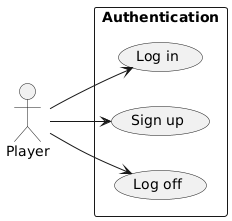
\includegraphics[keepaspectratio]{PSI_3rd_trial/packages/use_case_account.png}
    \caption{Authentication use case package diagram}
    \label{fig:authentication_package}
\end{figure}

\subsubsection{Log in}

\begin{figure}[H]
    \centering
    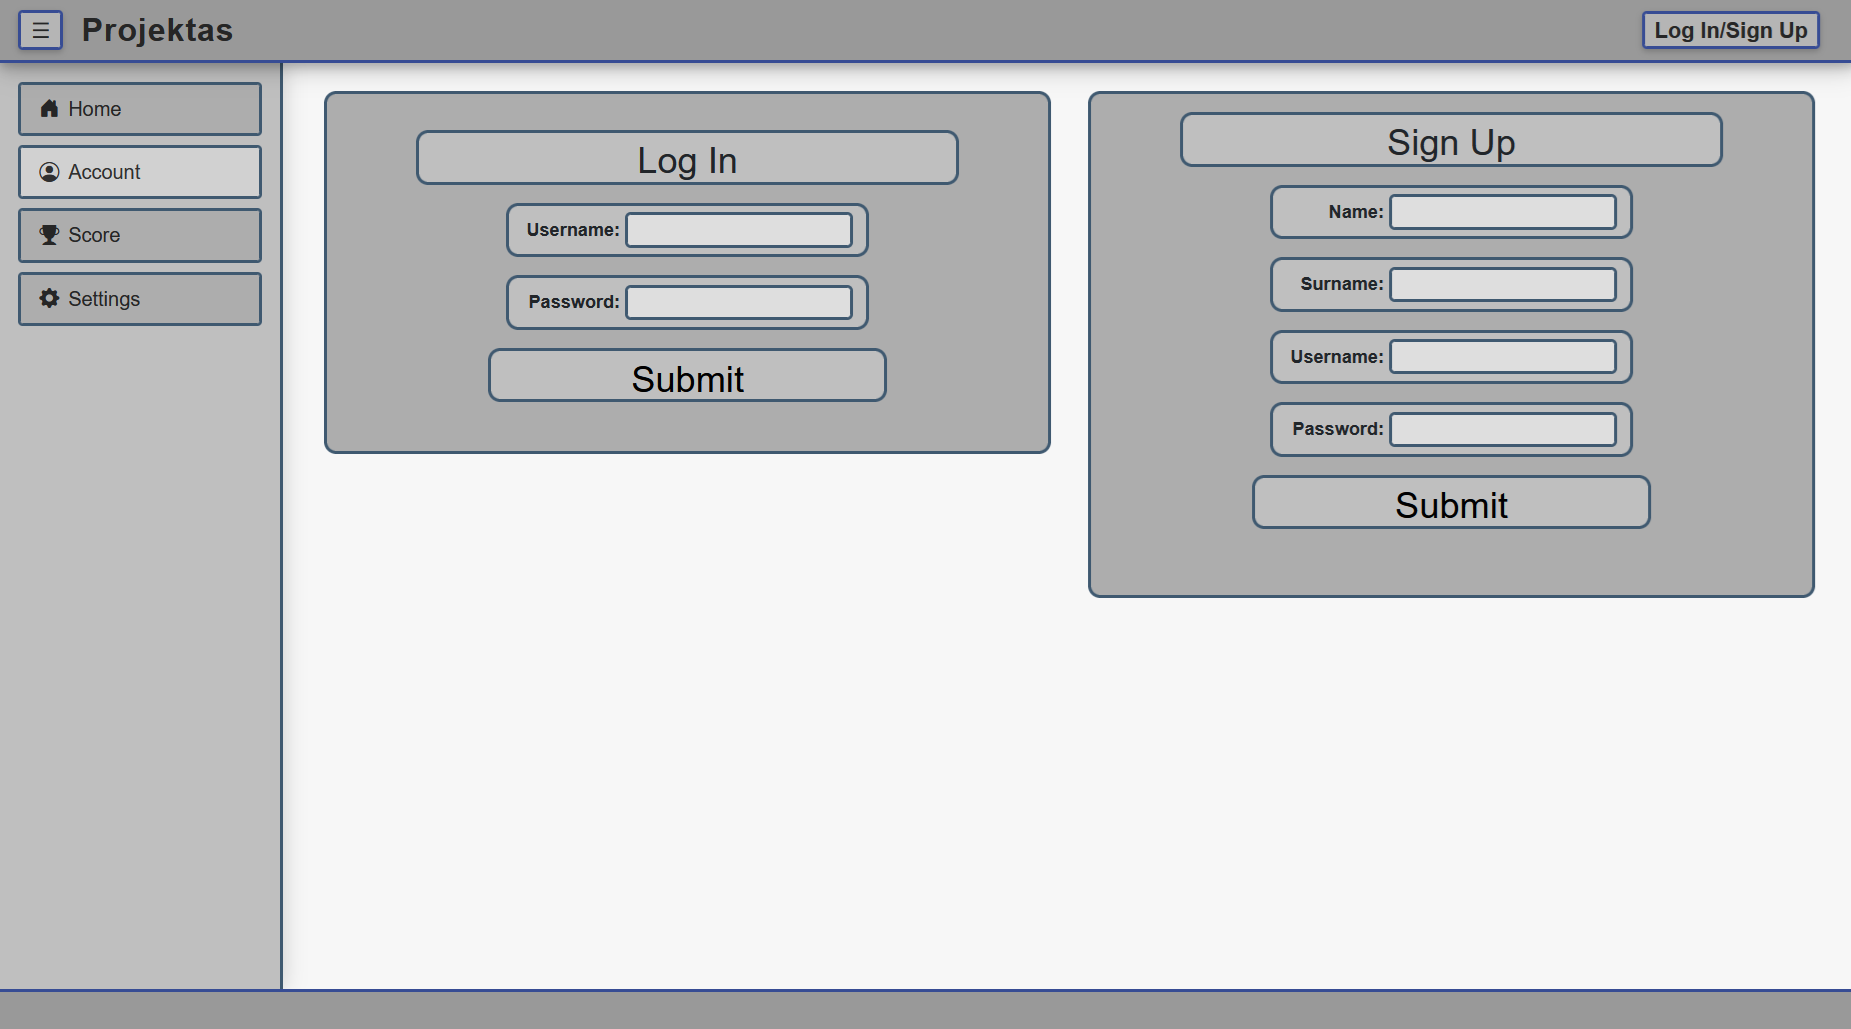
\includegraphics[width=1\textwidth,keepaspectratio]{PSI_3rd_trial/PNGs/log_in__signup.png}
    \caption{Account Page with Log In/Sign Up GUI}
    \label{fig:log_in}
\end{figure}

\heading{Basic course:}
The system displays the account page. The player types in his username and password in the fields displayed in the login section on the account page. The player clicks the submit button. The system checks if any fields are empty. The system checks player session if the player is already logged in. The system checks if a matching username and password combination exists in the player list. The system logs the player in (starts a player session). The System displays the home page and a message indicating that the login was successful.

\heading{Alternate course (some field was empty):}
The system displays the account page and a message indicating that a field was empty.

\heading{Alternate course (No matching combination was found):}
The system displays the account page and a message indicating that no such combination was found.

\heading{Alternate course (The player is already logged in):}
The system ignores the request and displays the home page.

\begin{figure}[H]
    \centering
    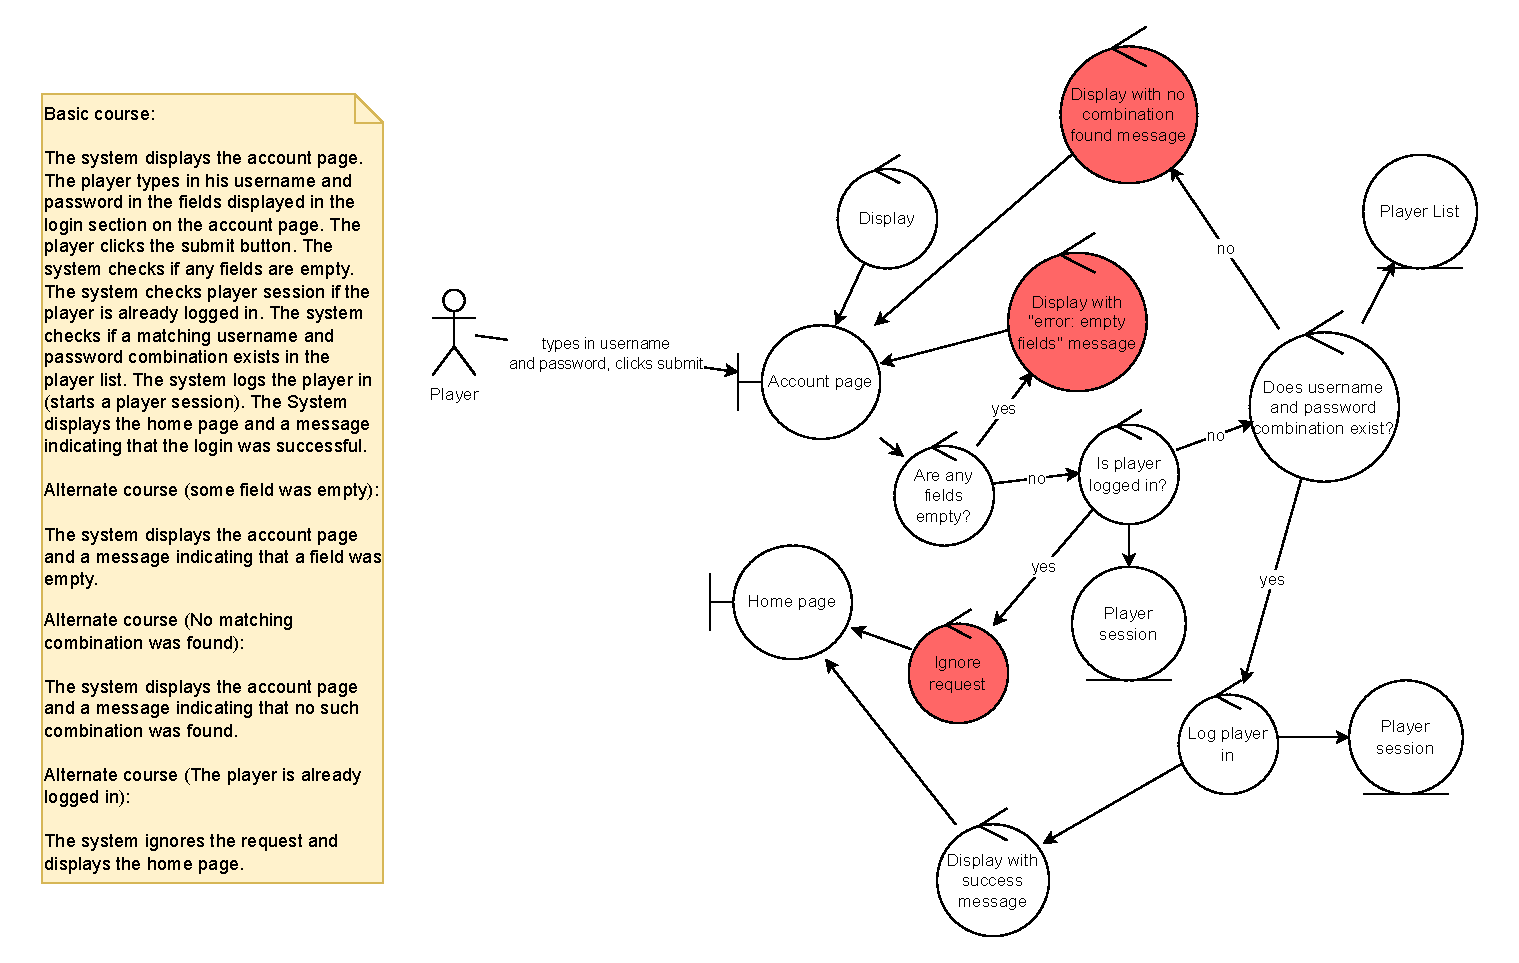
\includegraphics[width=1\textwidth,keepaspectratio]{robustness/log_in.drawio.pdf}
    \caption{Log In Robustness Diagram}
    \label{fig:log_in_robustness}
\end{figure}

This use case is derived from the Functional Requirements 1.a.

\subsubsection{Sign up}

\heading{Basic course:}
The system displays the account page. The player types in his name, surname, username, password in the fields displayed in the sign up section on the account page. The player clicks the submit button. The system checks if the player is already logged in. The system checks if the username exists in the player list and if the password matches security requirements (length, symbols used). The system creates a player account and stores it in the player list. The system displays the account page and a message indicating success.

\heading{Alternate course (player is logged in):}
The system ignores the request and displays the home page.

\heading{Alternate course (username not unique):}
The system displays the account page and a message stating that the operation failed because the username already exists.

\heading{Alternate course (password too weak):}
The system displays the account page and a message stating that the operation failed because the submitted password is too weak and a list of password requirements.

\begin{figure}[H]
    \centering
    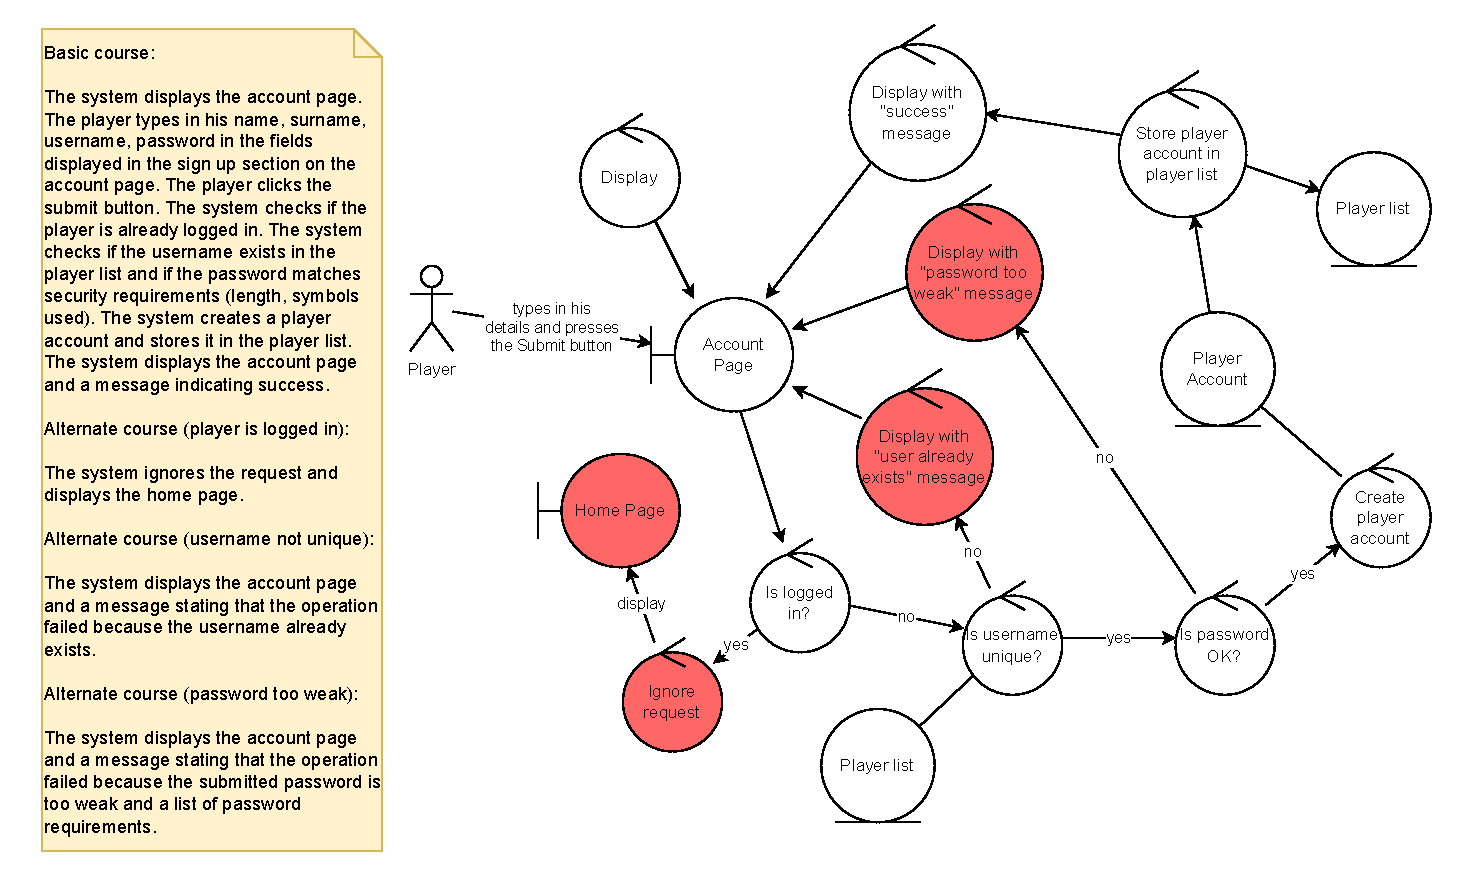
\includegraphics[width=1\textwidth,keepaspectratio]{robustness/sign_up.drawio.pdf}
    \caption{Sign Up Robustness Diagram}
    \label{fig:sign_up_robustness}
\end{figure}


This use case is derived from the section Functional Requirements 1.a.

\subsubsection{Log off}

\heading{Basic course:}
The system displays the account page. The player clicks the log off button.  The system checks if the player is logged in. The system logs the player off (kills the player session) and displays the home page with a message indicating success.

\begin{figure}[H]
    \centering
    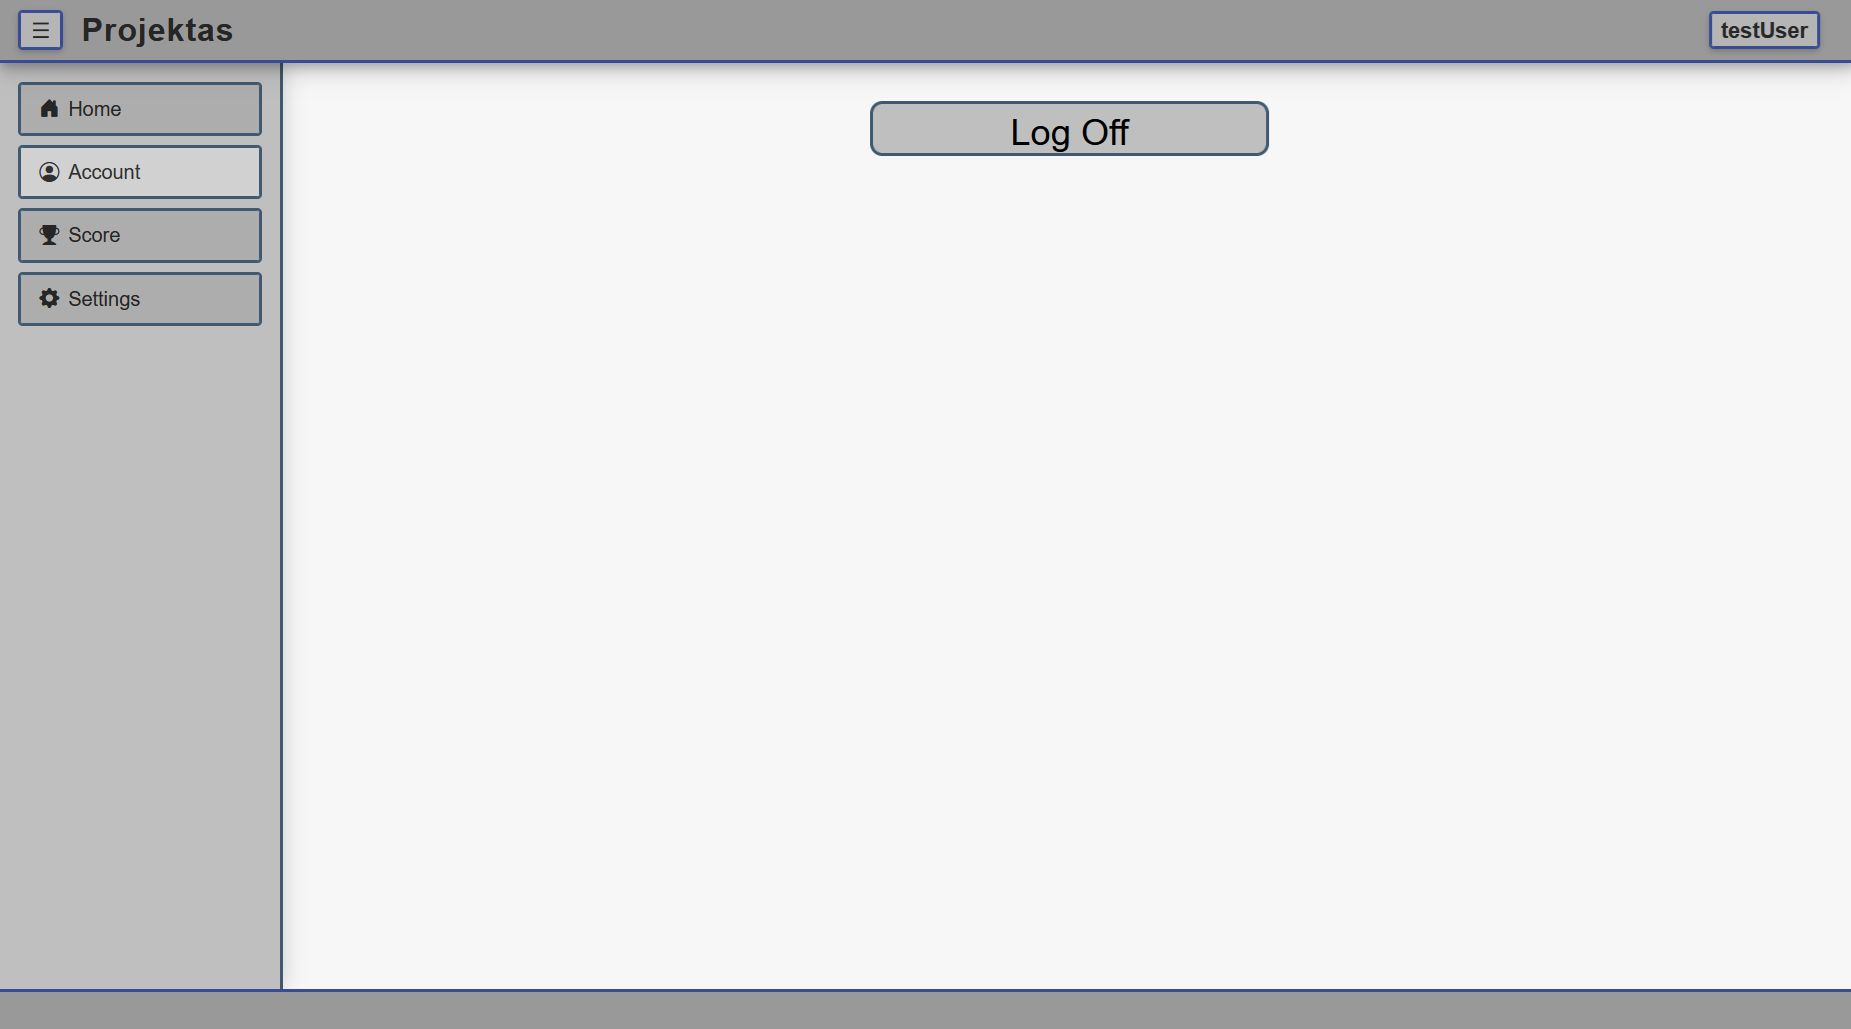
\includegraphics[width=1\textwidth,keepaspectratio]{PSI_3rd_trial/PNGs/log_off.png}
    \caption{Account Page with Log Off GUI}
    \label{fig:log_off}
\end{figure}

\heading{Alternate course (player is not logged in):}
The system ignores the request and displays the account page.

\begin{figure}[H]
    \centering
    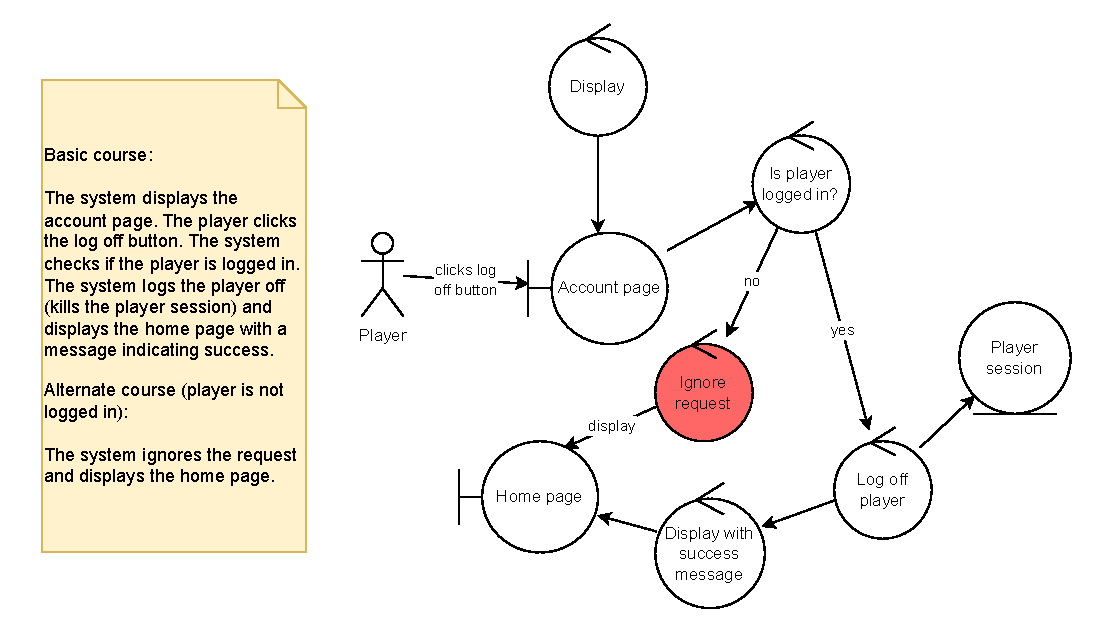
\includegraphics[width=1\textwidth,keepaspectratio]{robustness/log_off.drawio.pdf}
    \caption{Log Off Robustness Diagram}
    \label{fig:log_off_robustness}
\end{figure}

This use case is derived from the Functional Requirements 1.a.

\subsection{Game package}

\begin{figure}[H]
    \centering
    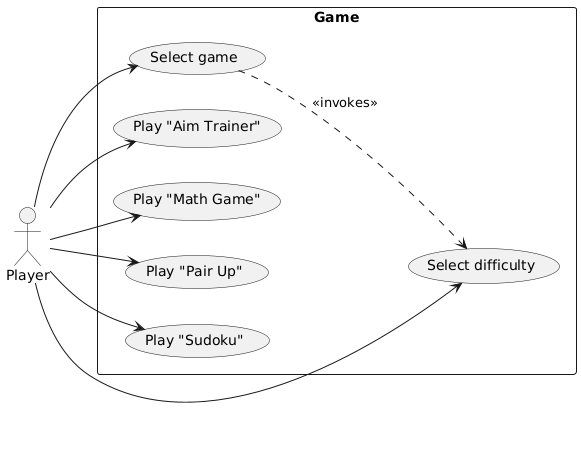
\includegraphics[width=1\textwidth,keepaspectratio]{PSI_3rd_trial/use_case_game_selection.png}
    \caption{Game use case package diagram}
    \label{fig:game_package}
\end{figure}

\subsubsection{Select Game}

\begin{figure}[H]
    \centering
    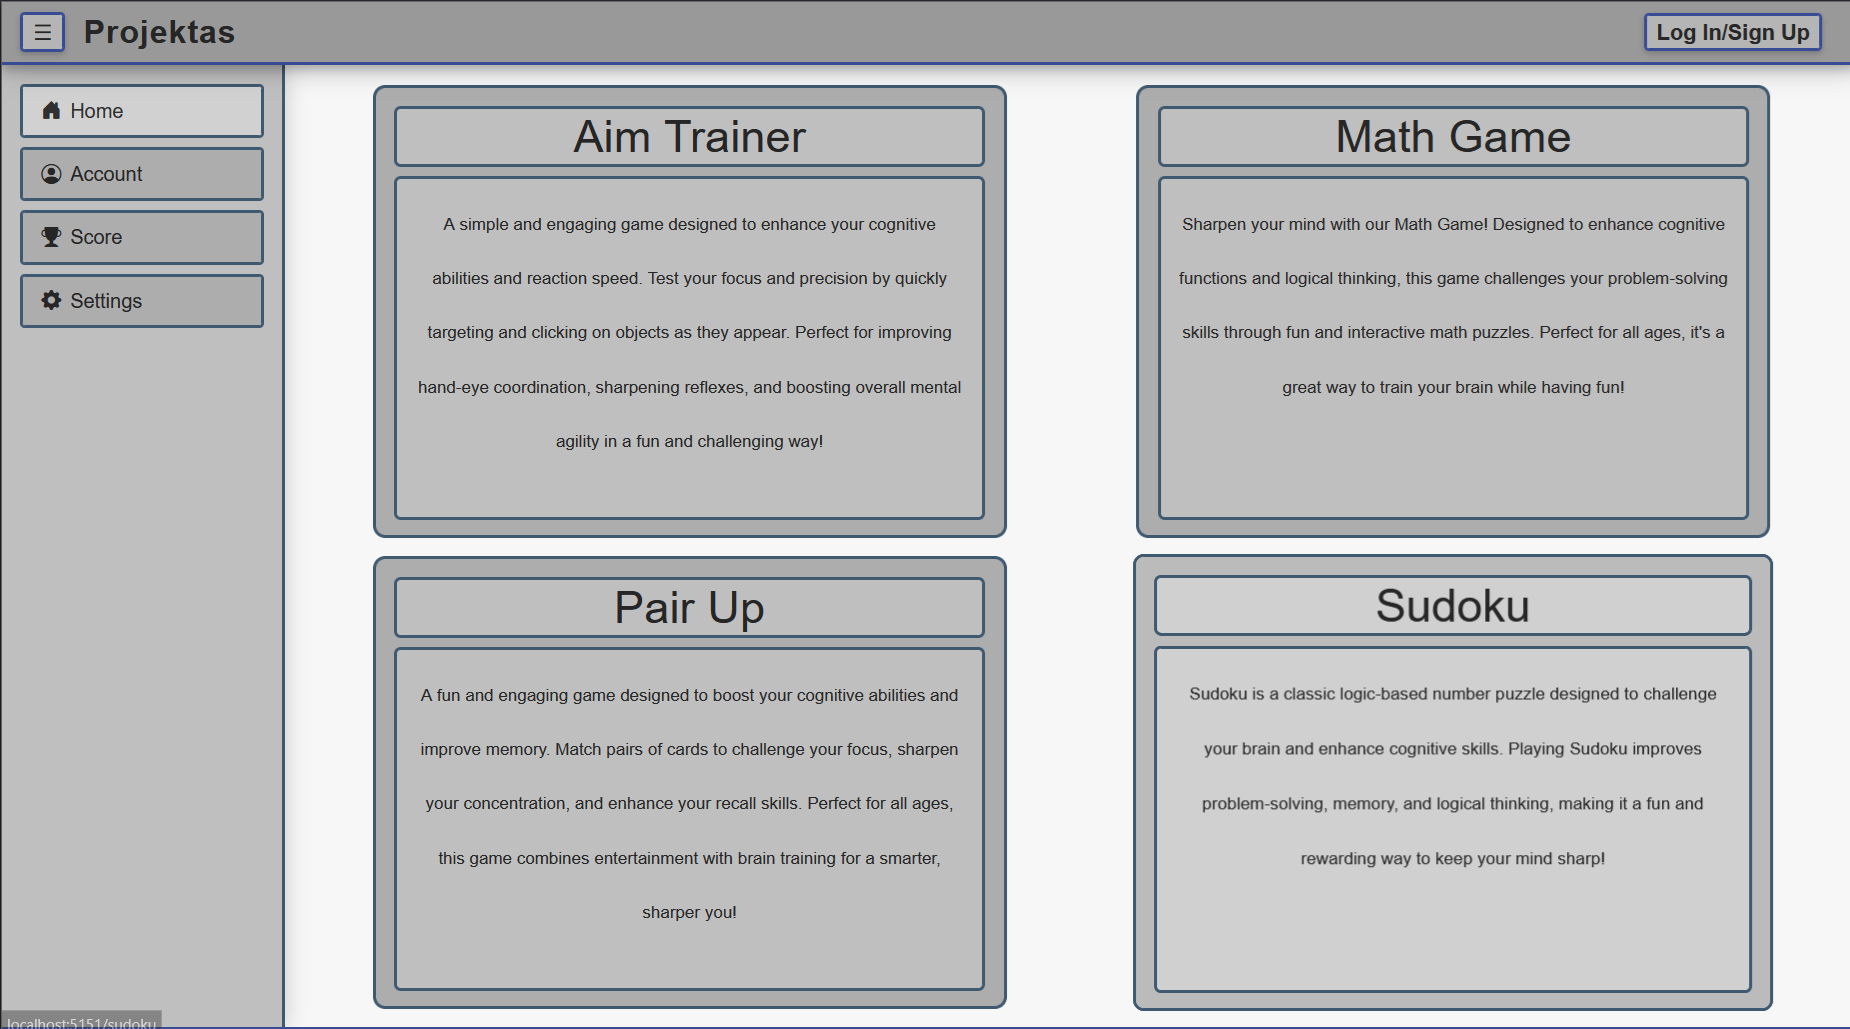
\includegraphics[width=1\textwidth,keepaspectratio]{PSI_3rd_trial/PNGs/game_selection.png}
    \caption{Game selection GUI}
    \label{fig:game_selection}
\end{figure}

\heading{Basic Course:}
The system displays the home page (which doubles as the game selection page) showing four large game selection buttons with the name and description of the game. The player presses one of the game selection buttons. The system checks which game was selected. The system displays the page for the selected game (invokes select difficulty).

\begin{figure}[H]
    \centering
    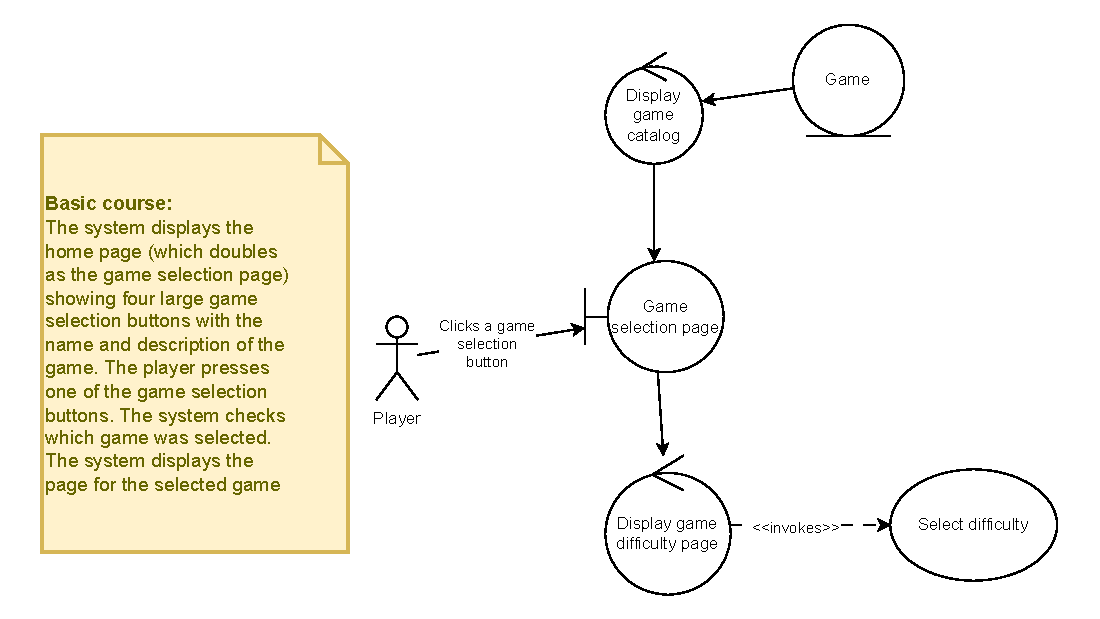
\includegraphics[width=1\textwidth,keepaspectratio]{PSI_3rd_trial/robustness/game_selection_good_2.drawio.pdf}
    \caption{Select Game Robustness Diagram}
    \label{fig:game_selection_diagram}
\end{figure}

This use case is derived from the Functional Requirements 1.b., 2., 3.a., 3.b.

\subsubsection{Select Difficulty}

\begin{figure}[H]
    \centering
    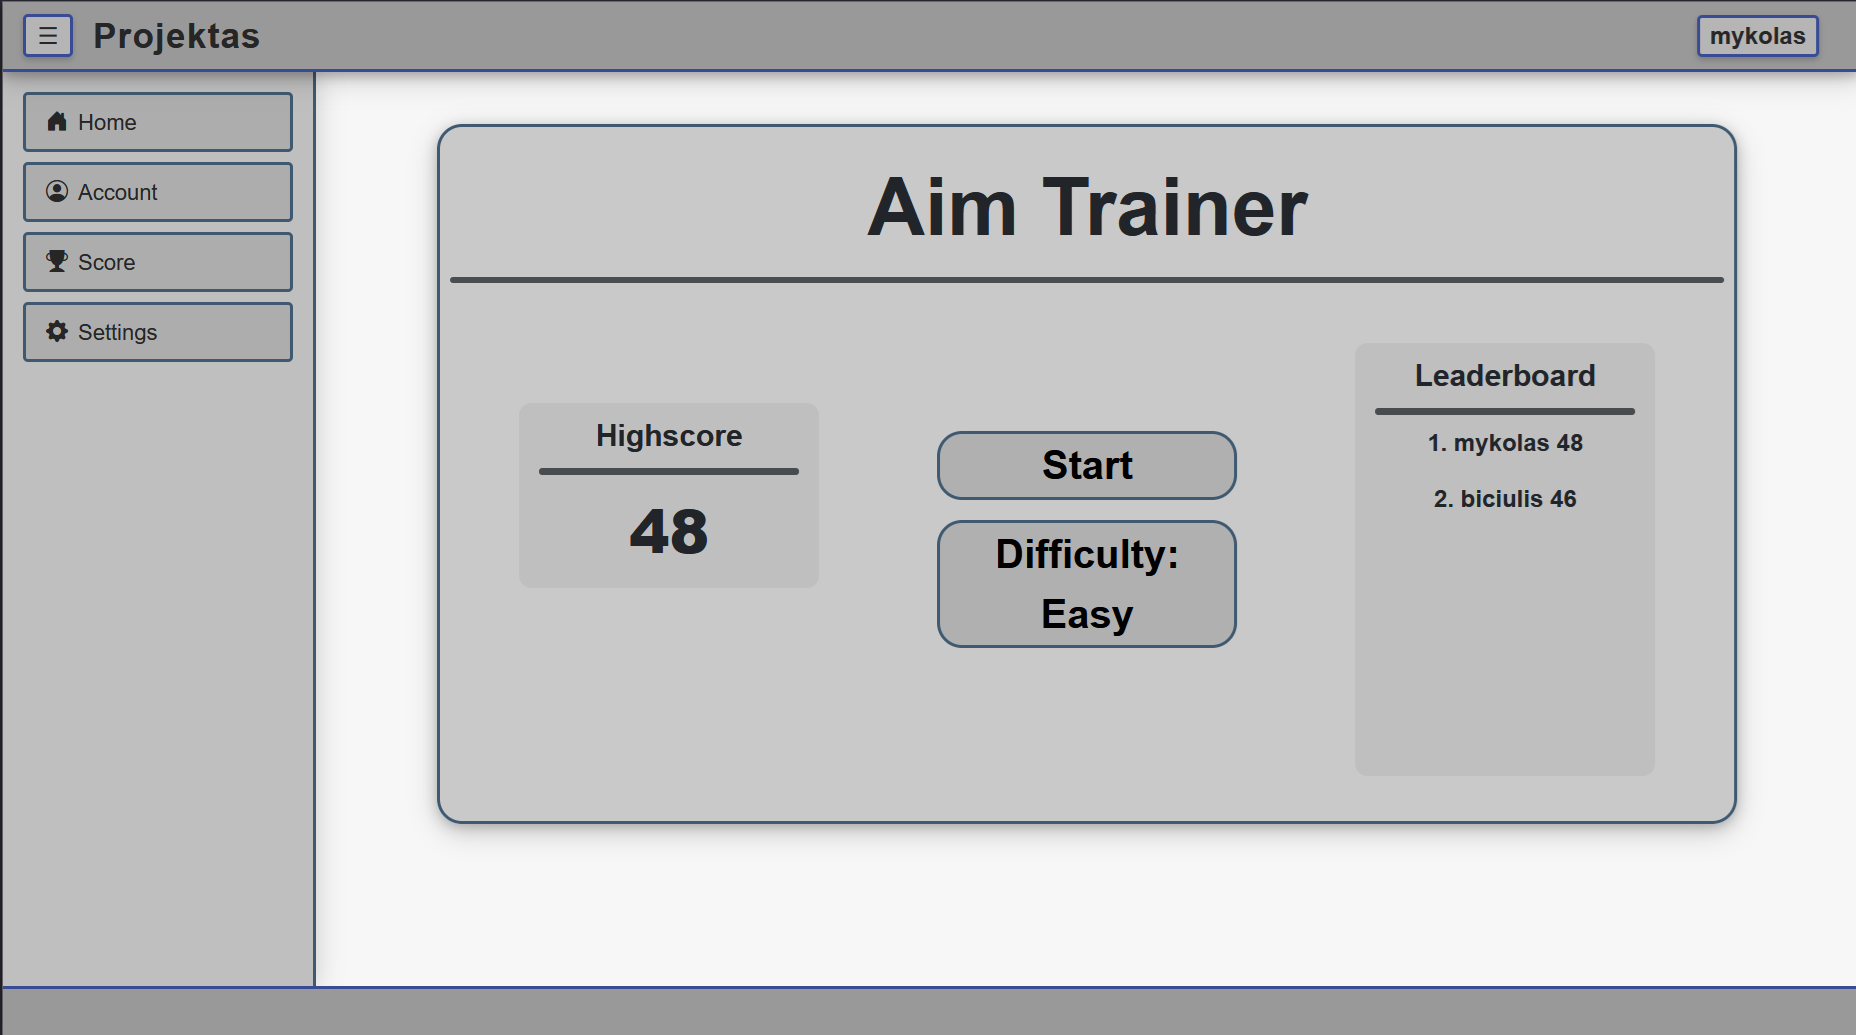
\includegraphics[width=1\textwidth,keepaspectratio]{PSI_3rd_trial/PNGs/select_difficulty.png}
    \caption{Game difficulty selection - easy}
    \label{fig:select_difficulty}
\end{figure}

\begin{figure}[H]
    \centering
    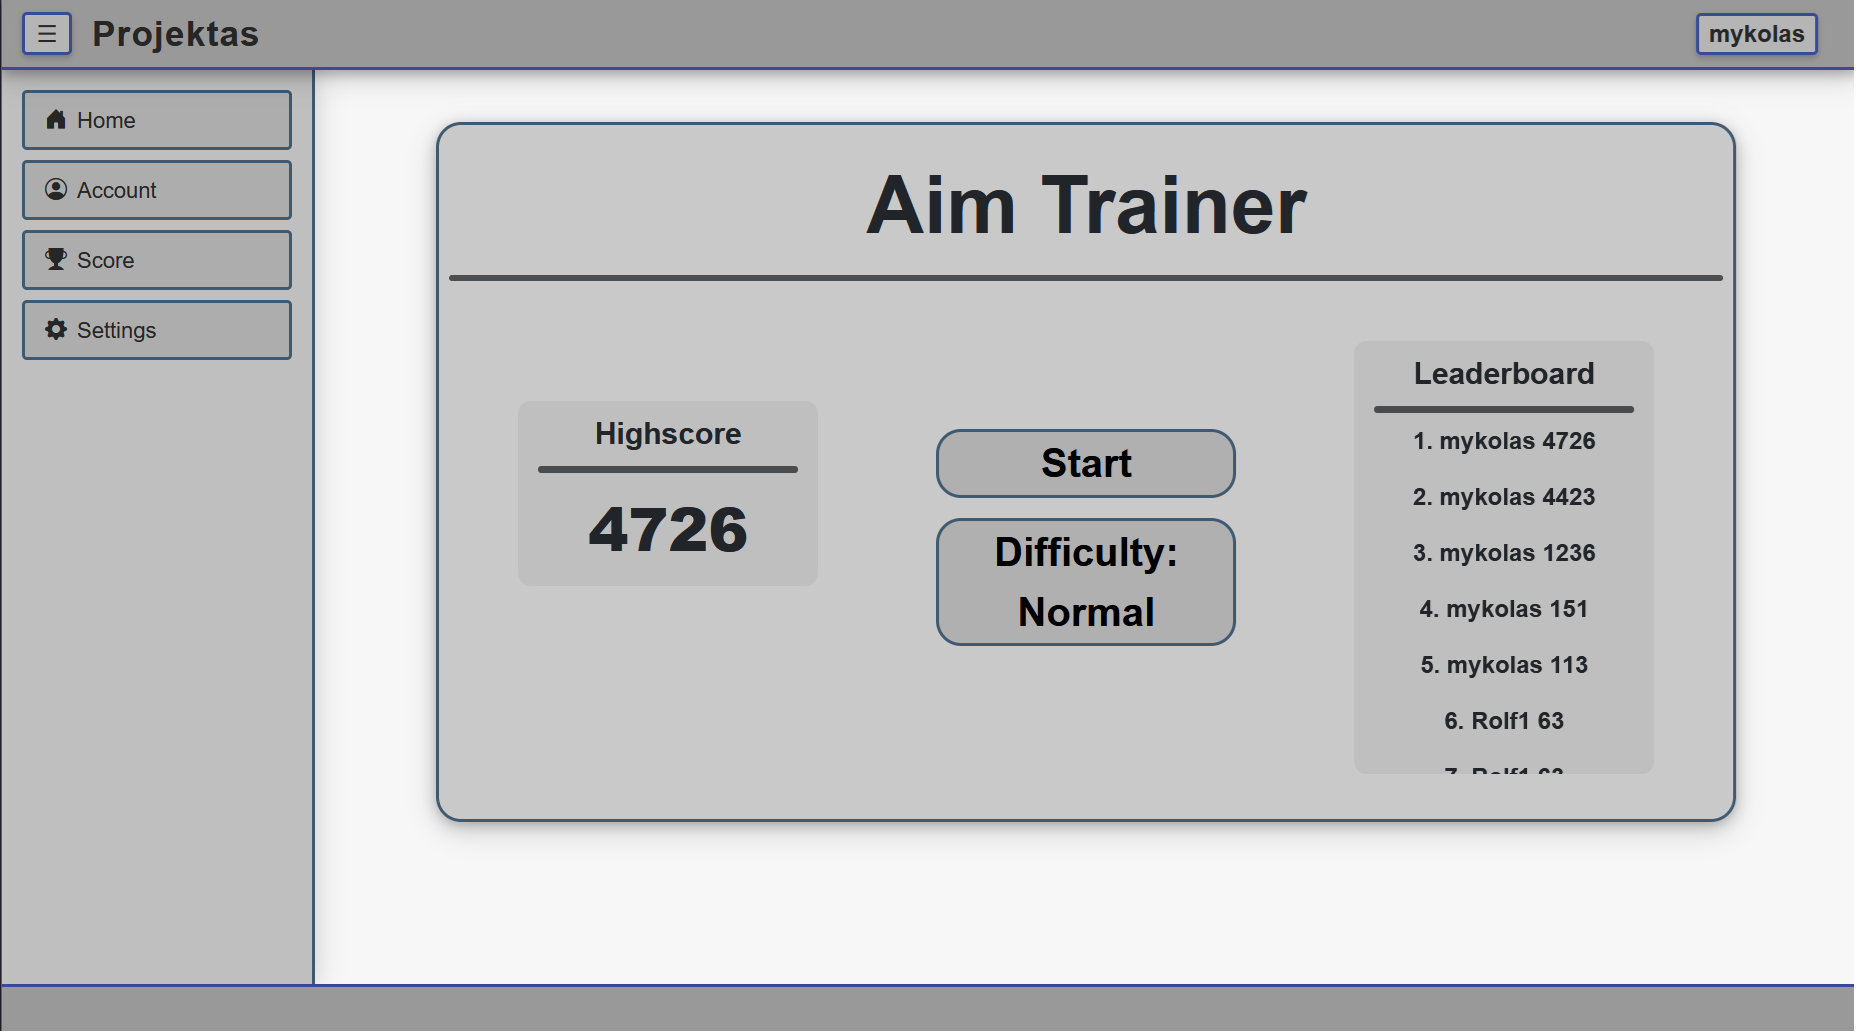
\includegraphics[width=1\textwidth,keepaspectratio]{PSI_3rd_trial/PNGs/select_difficulty_2.png}
    \caption{Game difficulty selection - normal}
    \label{fig:select_difficulty_2}
\end{figure}

\heading{Basic Course:}

Preceded by Select Game. The system displays two buttons: change difficulty and start game. The system sets the starting difficulty to easy. The player presses the change difficulty button. The system updates the game's difficulty to be "Normal" and the button's text is updated to be "Difficulty: Normal". The player presses the change difficulty button. The system updates the game's difficulty to be "Hard" and the button's text is updated to be "Difficulty: Hard". The player presses the start game button. System proceeds to take the player to the gameplay page.

\heading{Alternate Course (Player does not change difficulty):}
Player proceeds to start the game without changing difficulty.

\heading{Alternate Course (Player selects hard difficulty):}
Player proceeds to change the difficulty and changes it from "Hard" to "Easy" then starts the game.

\begin{figure}[H]
    \centering
    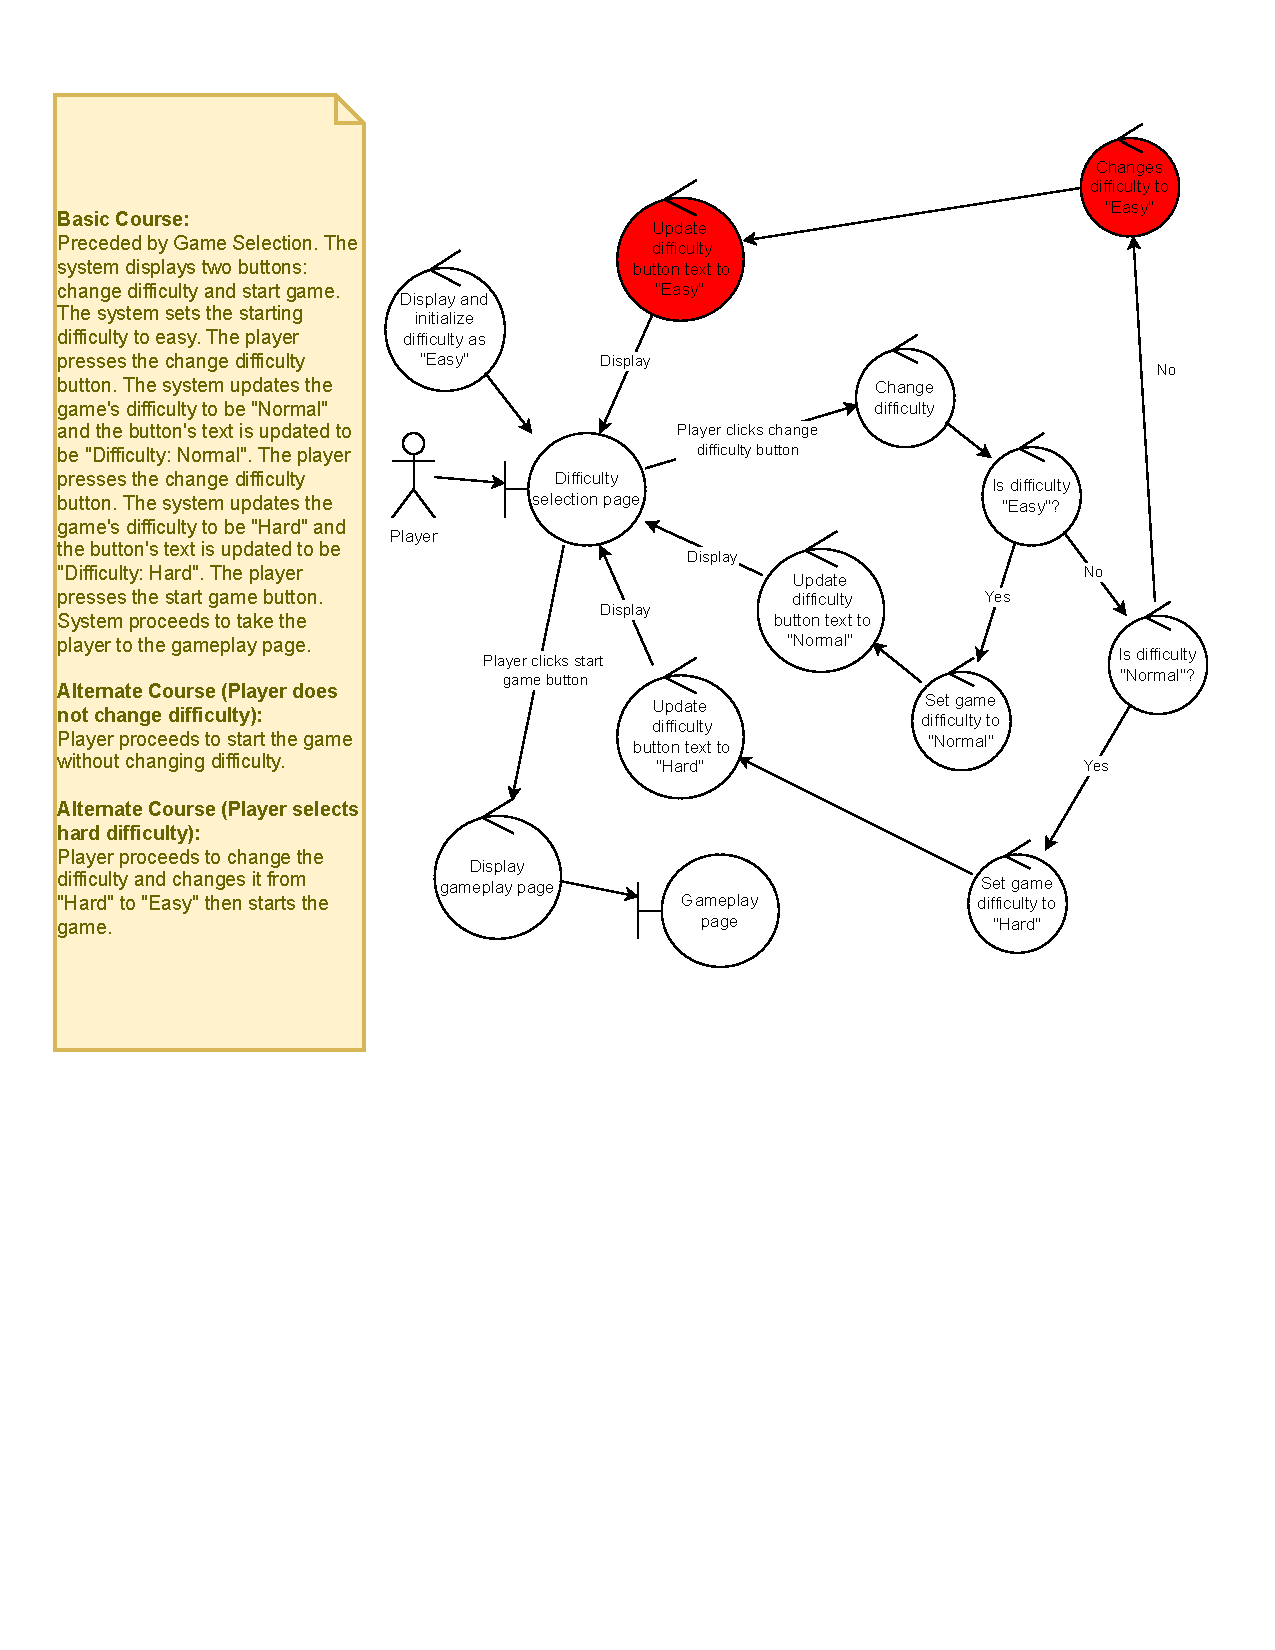
\includegraphics[width=1\textwidth,keepaspectratio]{PSI_3rd_trial/robustness/difficulty_selection.drawio.pdf}
    \caption{Select Difficulty Robustness Diagram}
    \label{fig:select_difficulty_robustness}
\end{figure}


This use case is derived from the Functional Requirements 3.b.


\subsubsection{Play Pair-Up}
% Include the detail that a score is displayed after the game ends. 3.f.
% Include the detail that the leaderboards get updated after a player with an account finishes a game. 3.g.

\begin{figure}[H]
    \centering
    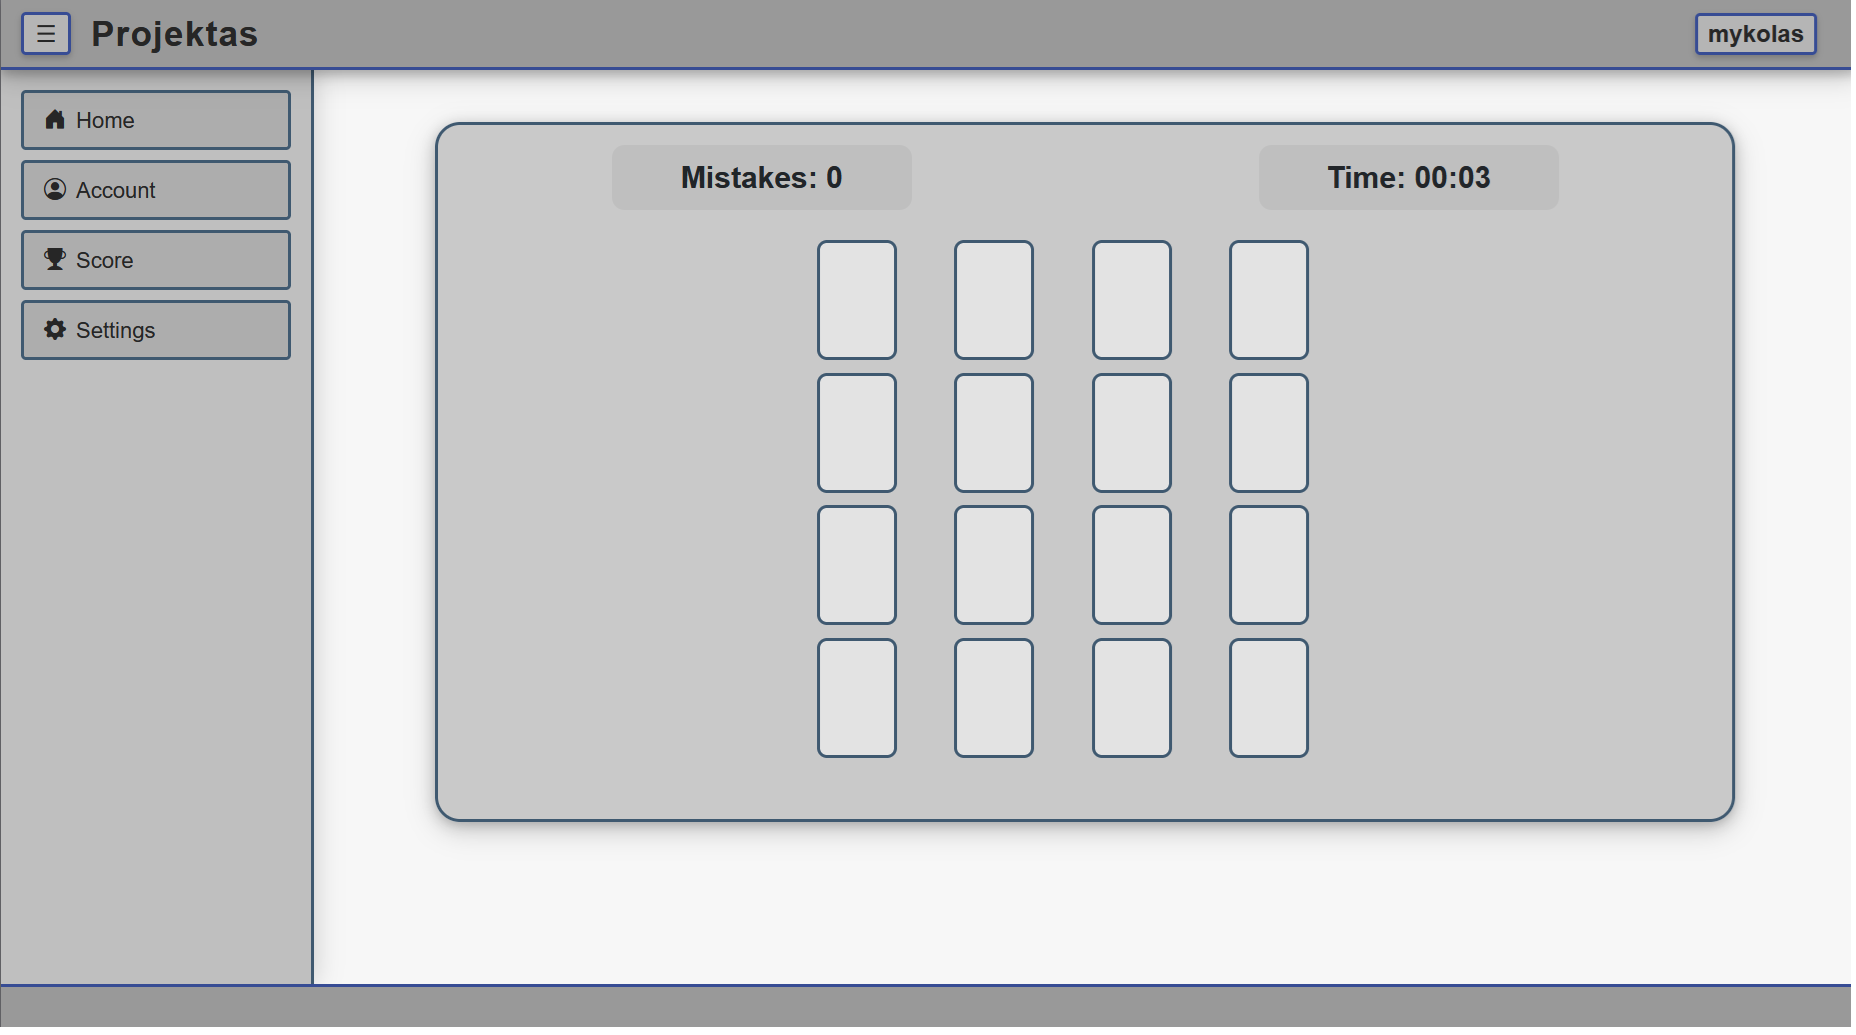
\includegraphics[width=1\textwidth,keepaspectratio]{PSI_3rd_trial/PNGs/pair_up_1.png}
    \caption{Pair Up game initial GUI}
    \label{fig:pair_up_1}
\end{figure}

\begin{figure}[H]
    \centering
    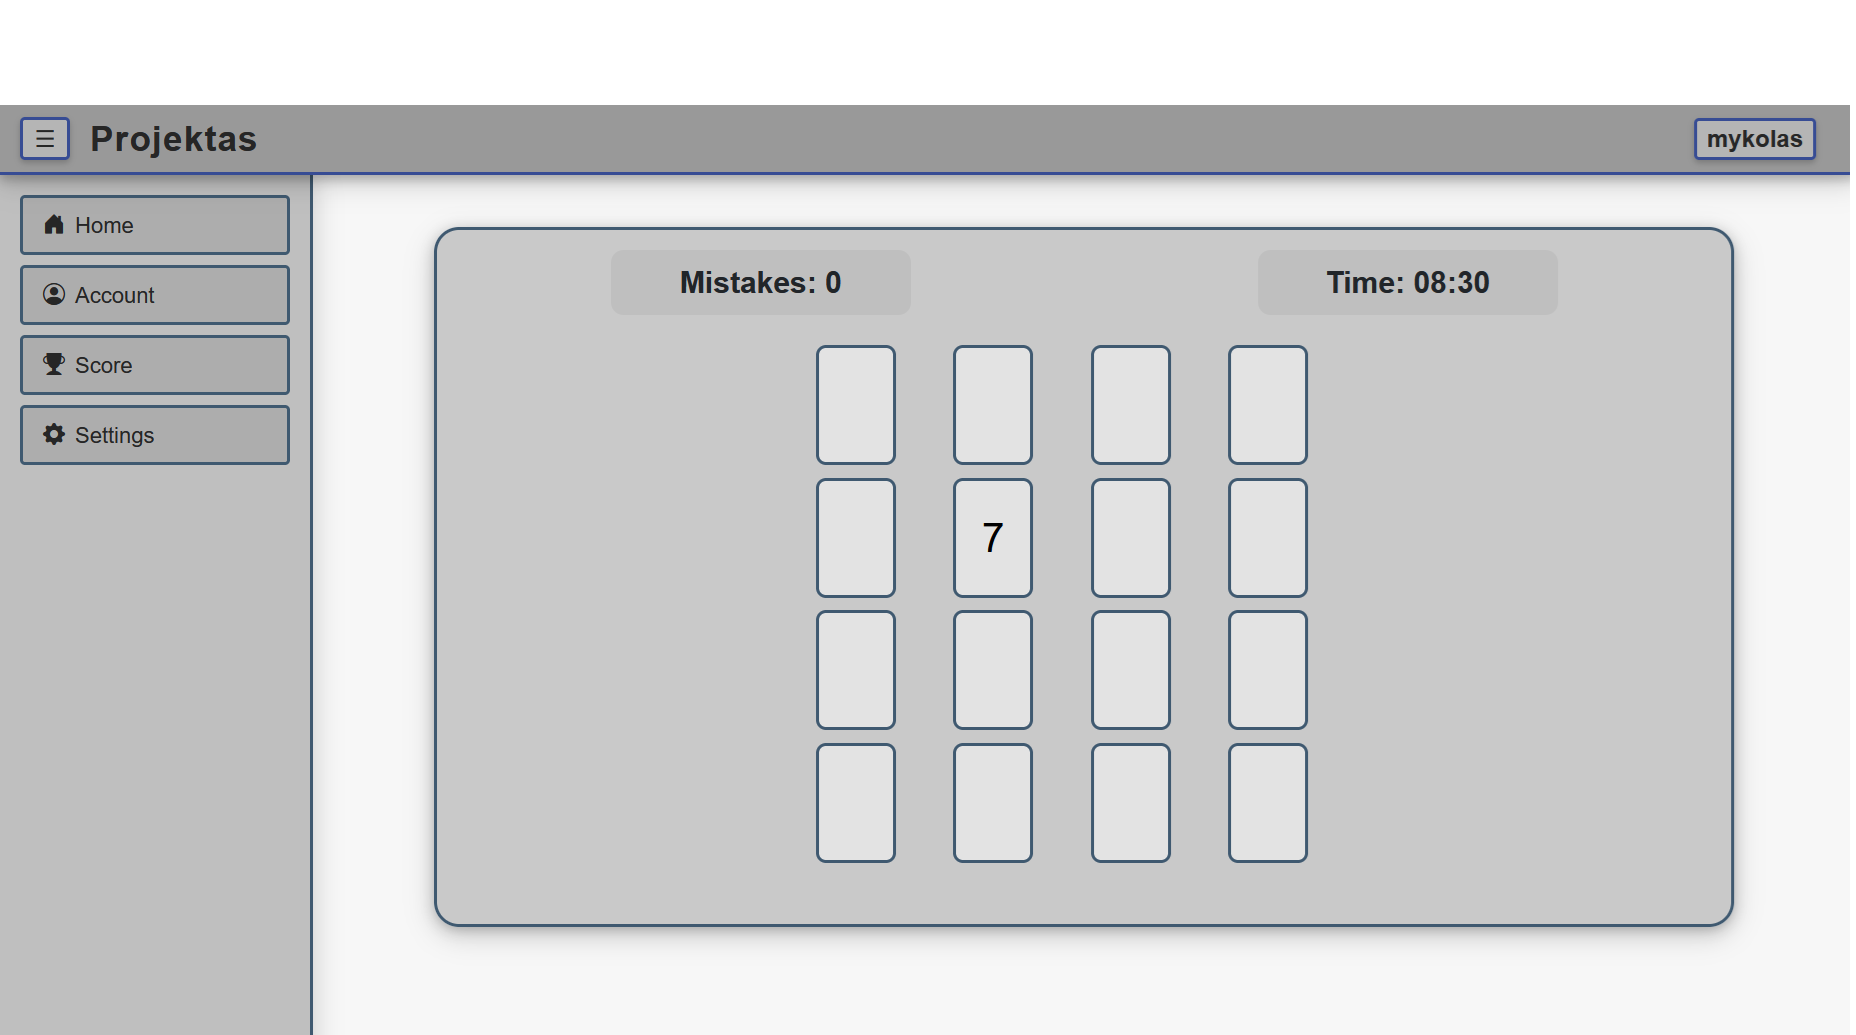
\includegraphics[width=1\textwidth,keepaspectratio]{PSI_3rd_trial/PNGs/pair_up_2.png}
    \caption{Pair Up game with one card selected GUI}
    \label{fig:pair_up_2}
\end{figure}


\begin{figure}[H]
    \centering
    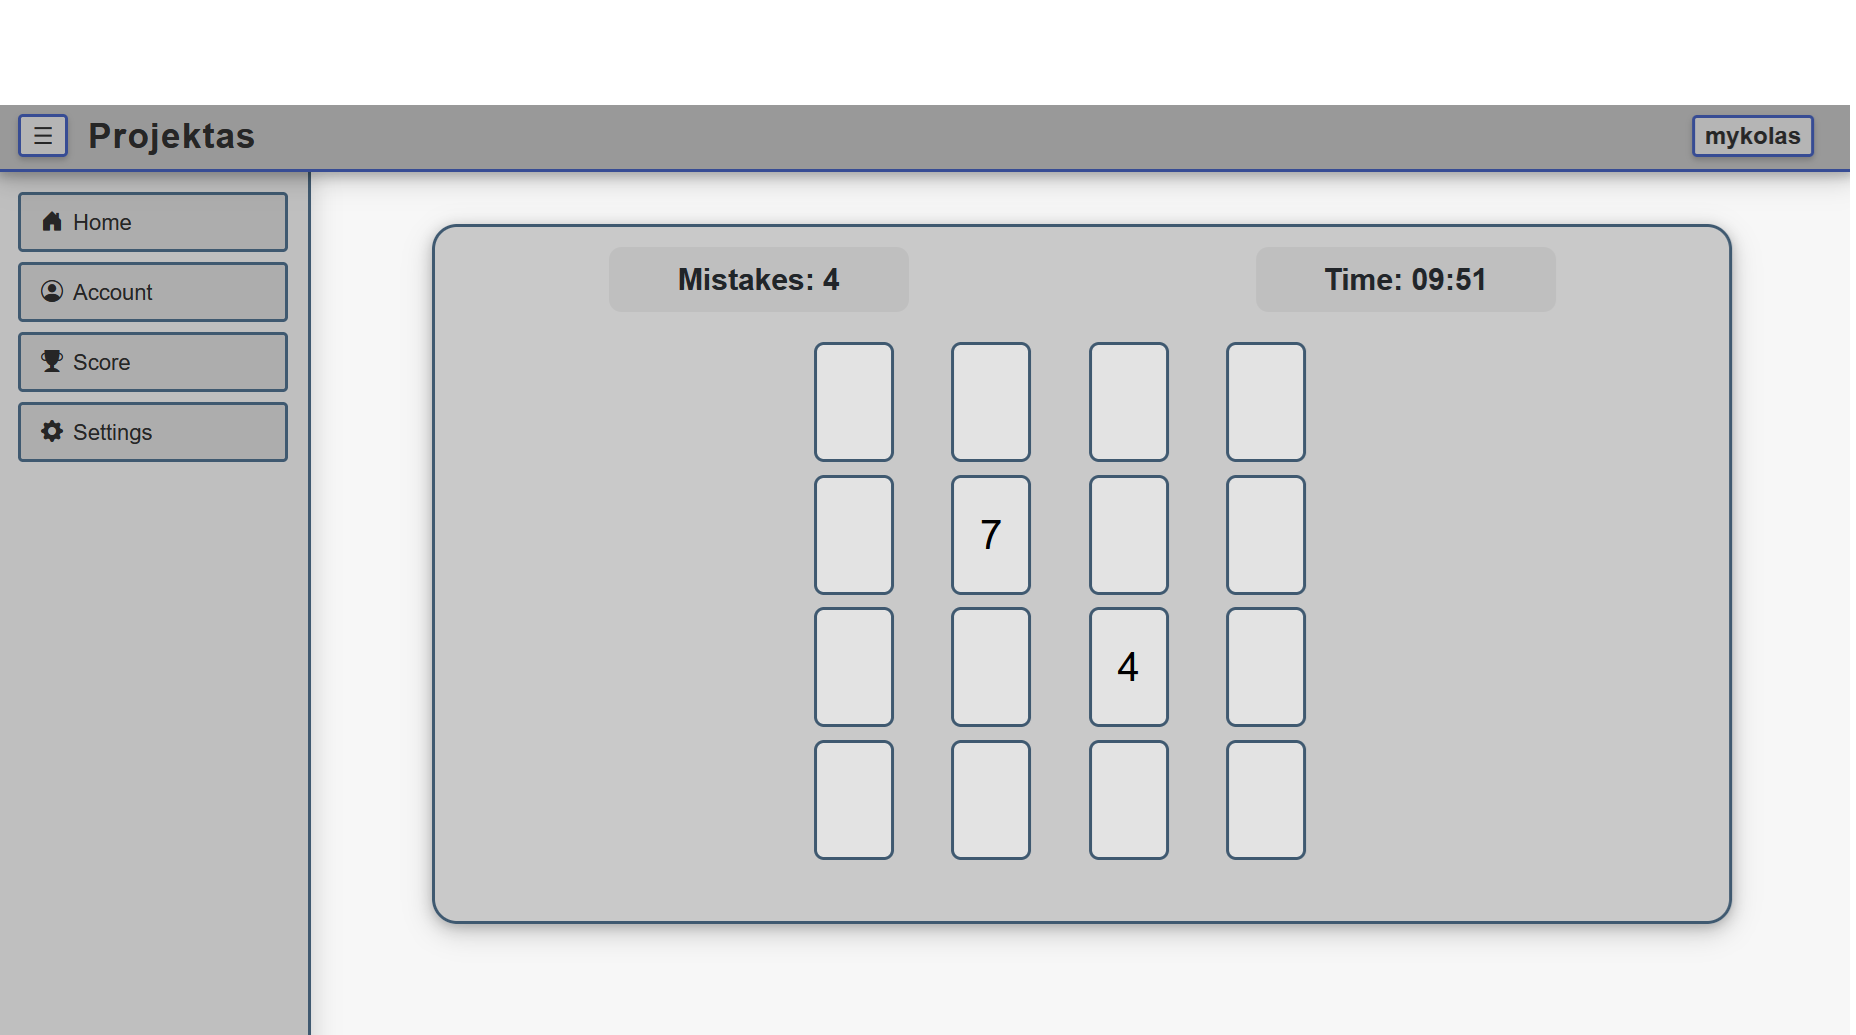
\includegraphics[width=1\textwidth,keepaspectratio]{PSI_3rd_trial/PNGs/pair_up_3.png}
    \caption{Pair Up game with two cards selected GUI}
    \label{fig:pair_up_3}
\end{figure}

\begin{figure}[H]
    \centering
    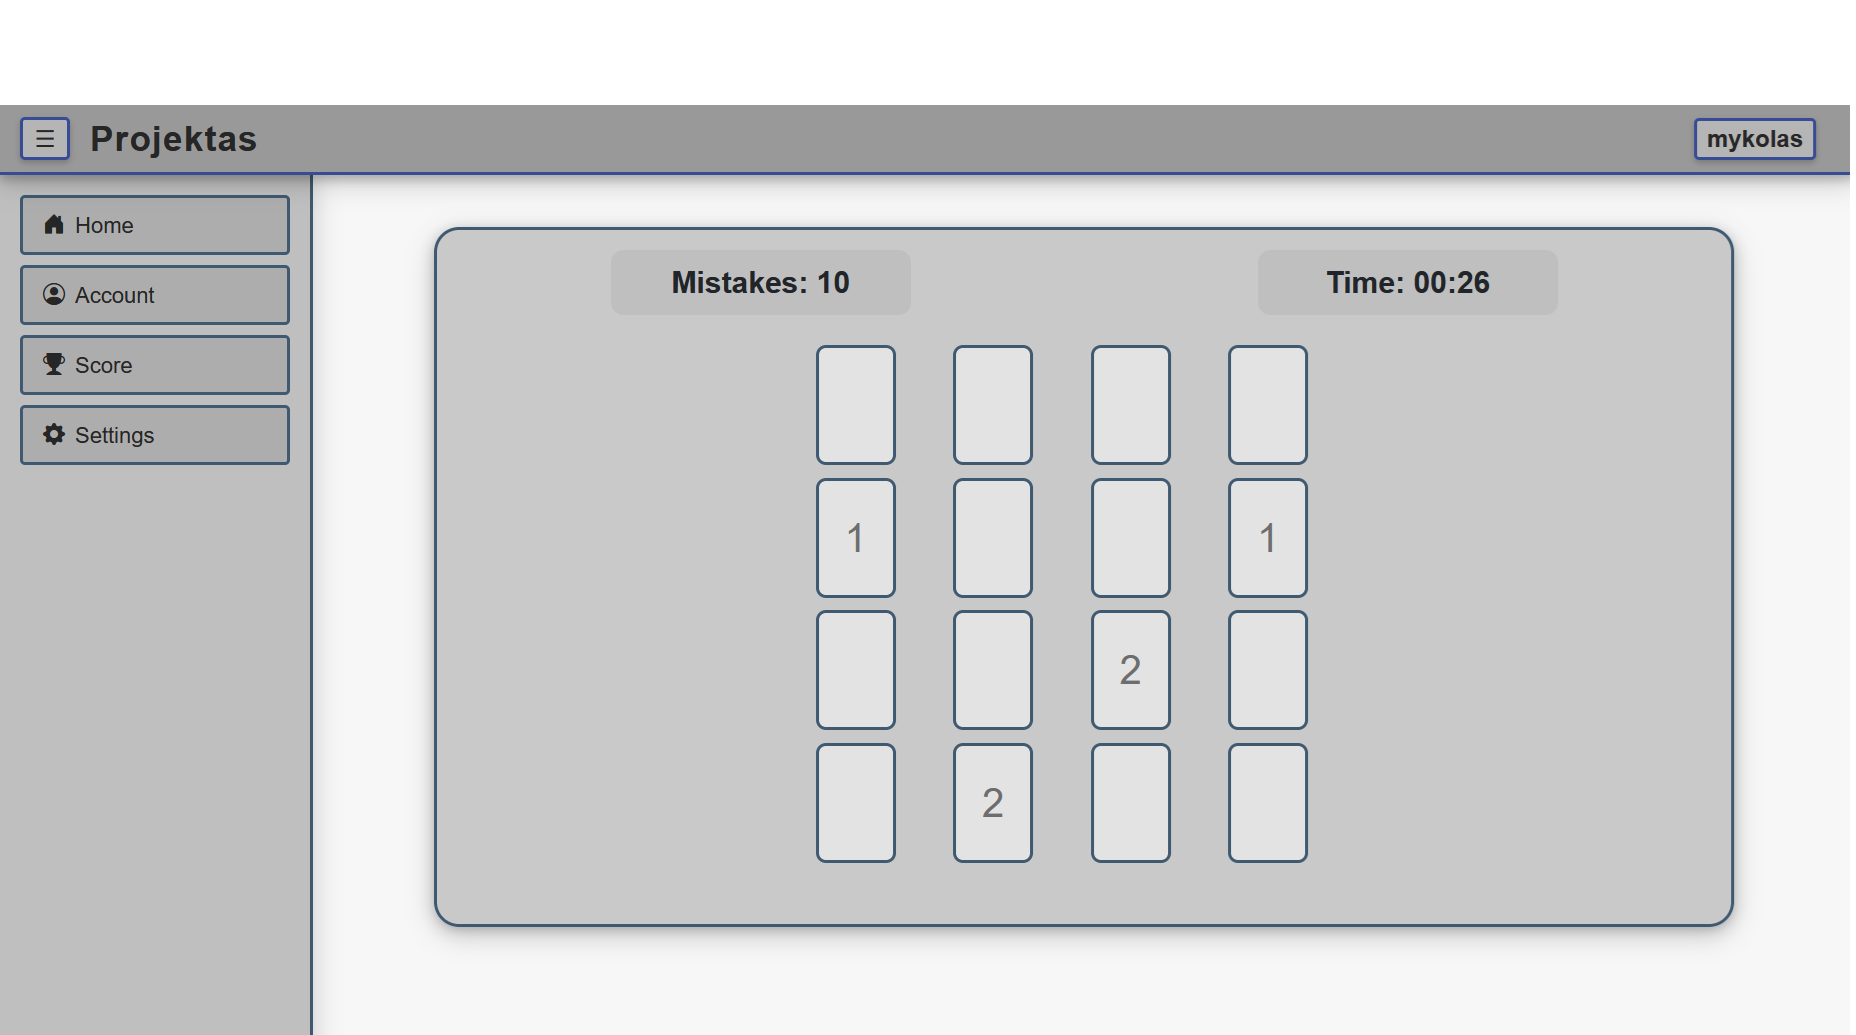
\includegraphics[width=1\textwidth,keepaspectratio]{PSI_3rd_trial/PNGs/pair_up_4.png}
    \caption{Pair up game with four cards locked GUI}
    \label{fig:pair_up_4}
\end{figure}

\begin{figure}[H]
    \centering
    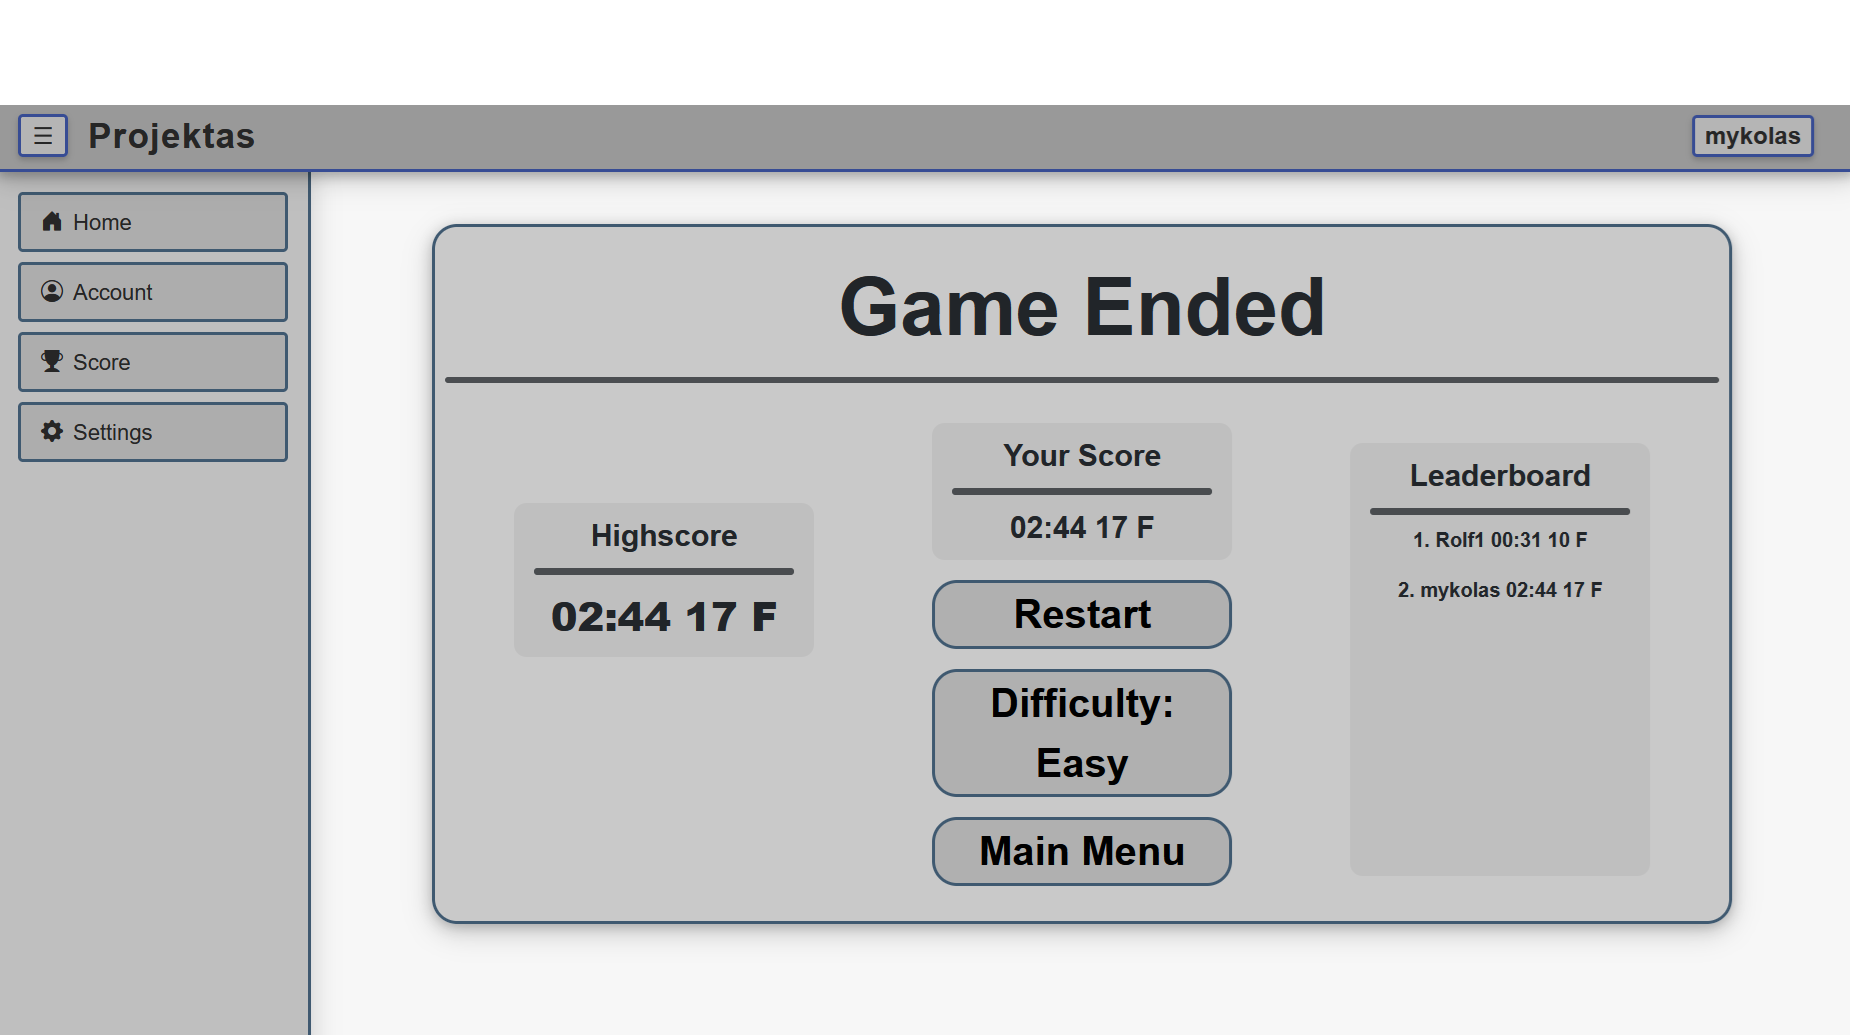
\includegraphics[width=1\textwidth,keepaspectratio]{PSI_3rd_trial/PNGs/pair_up_5.png}
    \caption{Pair up page GUI after the game ends}
    \label{fig:pair_up_5}
\end{figure}

\heading{Basic Course:}
The system initializes the Pair-Up gameplay page. The system shows two labels, one with a timer and one with a mistake count. Player selects a card. The system reveals a card symbol on the selected card. Player then selects a different card, the system reveals the card symbol of the second card. The system checks if the symbols on the cards match. The system locks in the card pair because it matches. The system checks if there are selectable cards remaining (has the pair-up game been won); if there are not any left, it displays the Pair-Up Page with the mistake count and the system saves the players score as the high score entry.

\heading{Alternate Course (Symbols do not match):}
Player selects two cards with different symbols. The system increases the mistake count and increments the mistakes counter. The system updates the displayed mistakes counter for the user.

\heading{Alternate Course (Player is logged out):}
The player is logged out and playing the game. After finishing the game the system does not save the player's score in the database.

\begin{figure}[H]
    \centering
    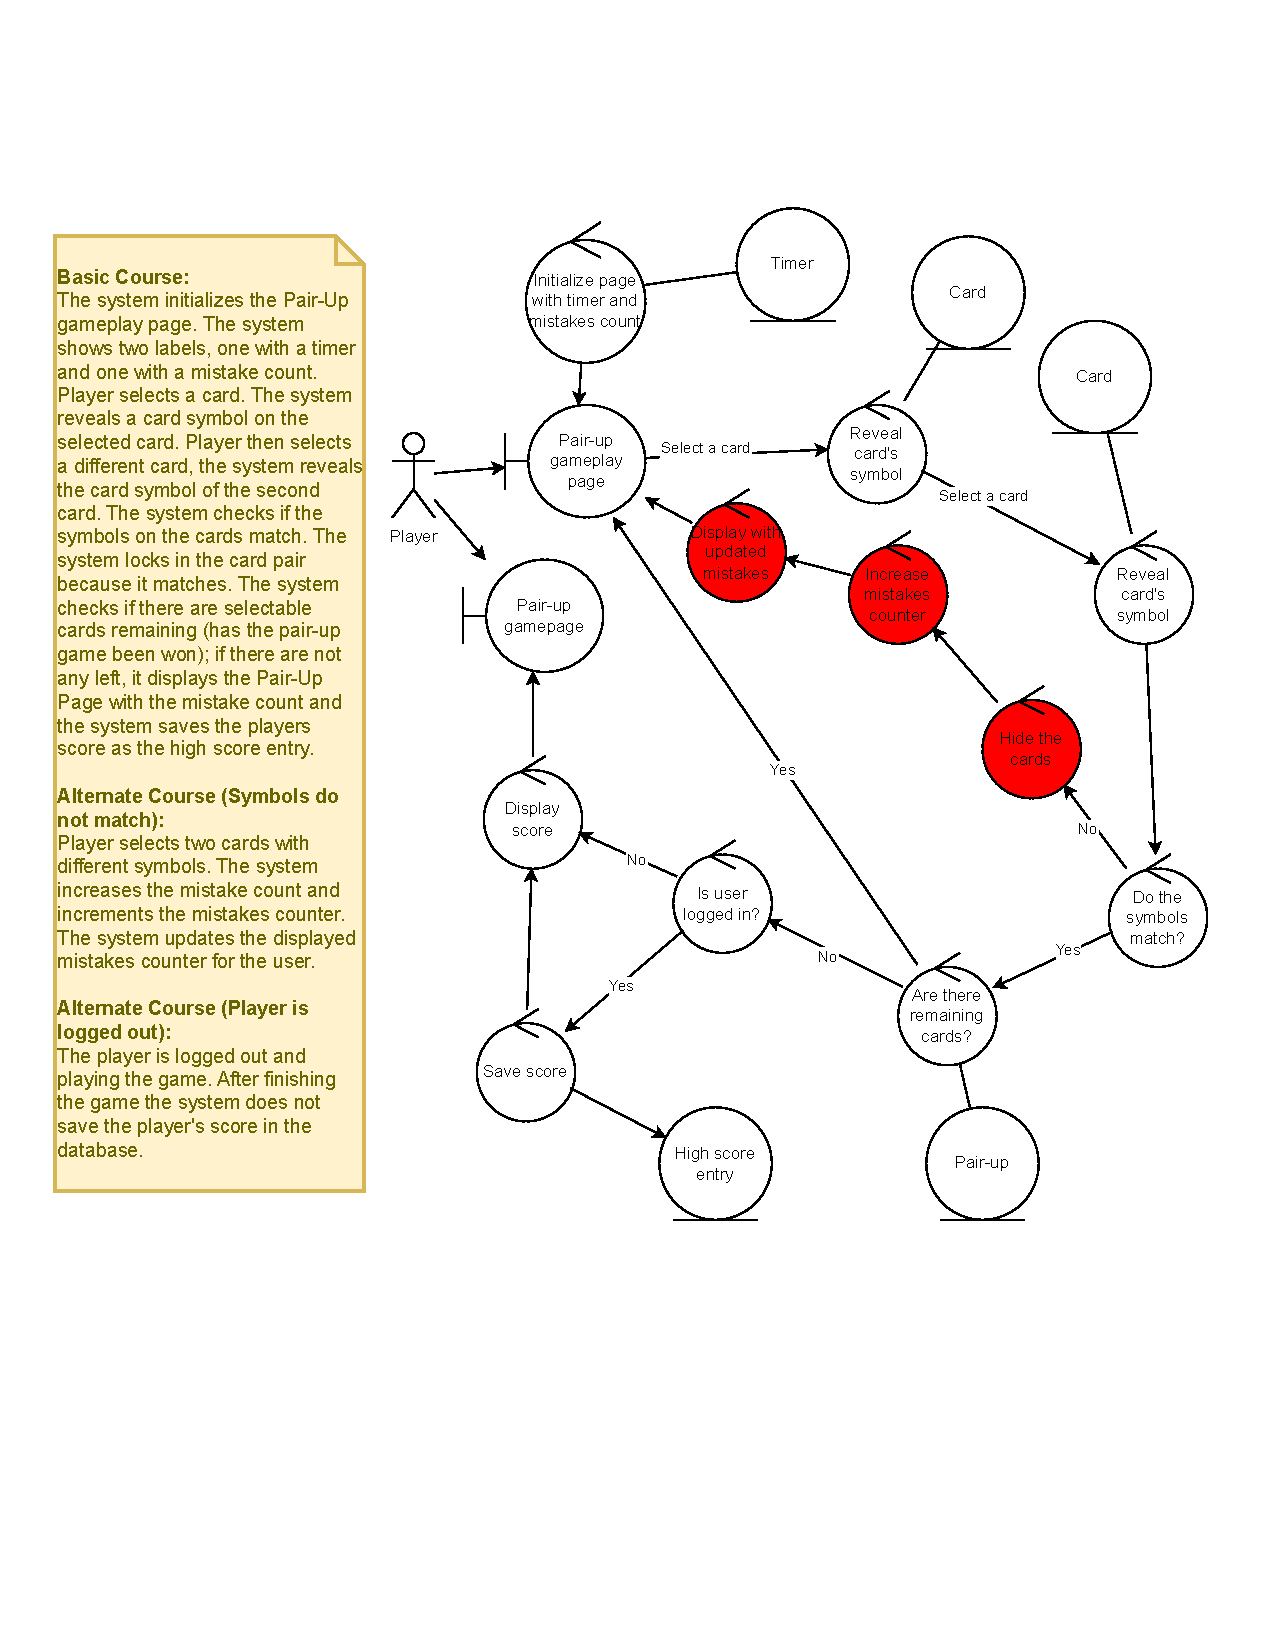
\includegraphics[width=1\textwidth,keepaspectratio]{PSI_3rd_trial/robustness/pair_up.drawio.pdf}
    \caption{Pair Up Robustness Diagram}
    \label{fig:pair_up_robustness}
\end{figure}

This use case is derived from the Functional Requirements 2.b., 3.c., 3.d., 3.f., 3.g.

\subsubsection{Play Aim Trainer}

% Include the detail that a score is displayed after the game ends. 3.f.
% Include the detail that the leaderboards get updated after a player with an account finishes a game. 3.g.

\begin{figure}[H]
    \centering
    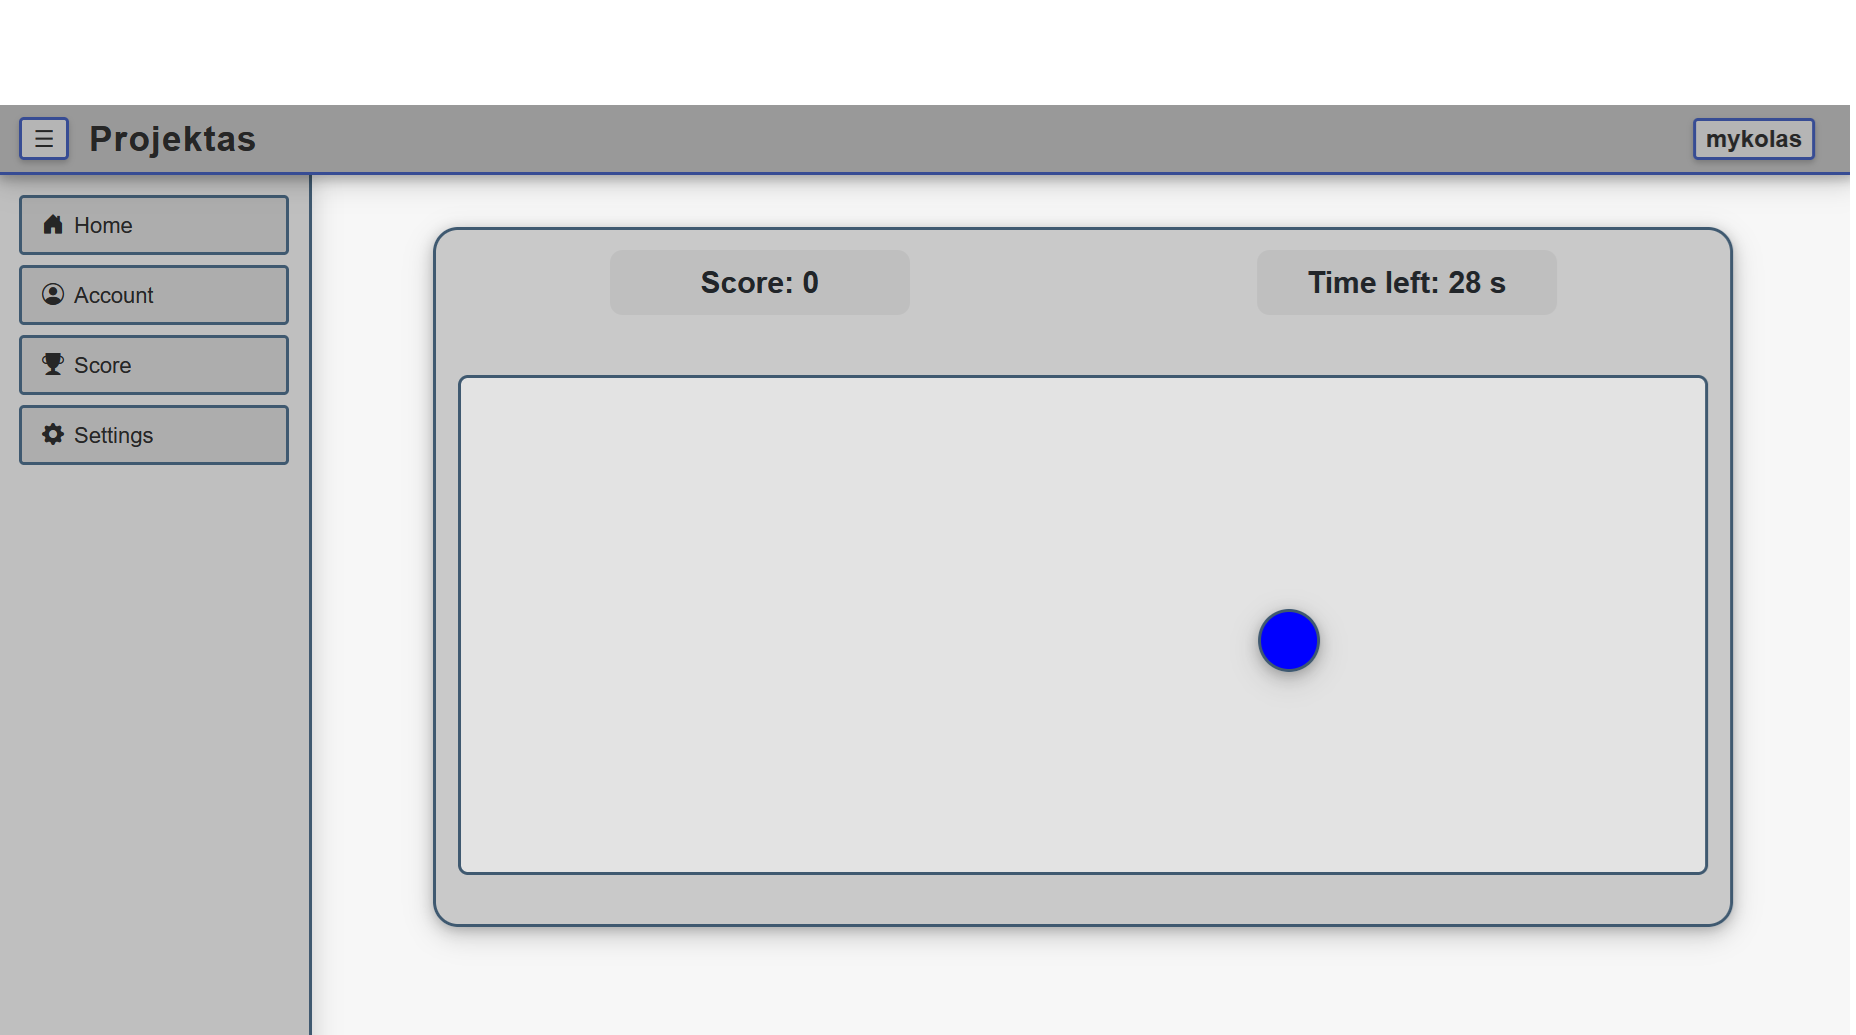
\includegraphics[width=1\textwidth,keepaspectratio]{PSI_3rd_trial/PNGs/aim_trainer_1.png}
    \caption{Aim Trainer gameplay page initial GUI}
    \label{fig:aim_trainer_1}
\end{figure}

\begin{figure}[H]
    \centering
    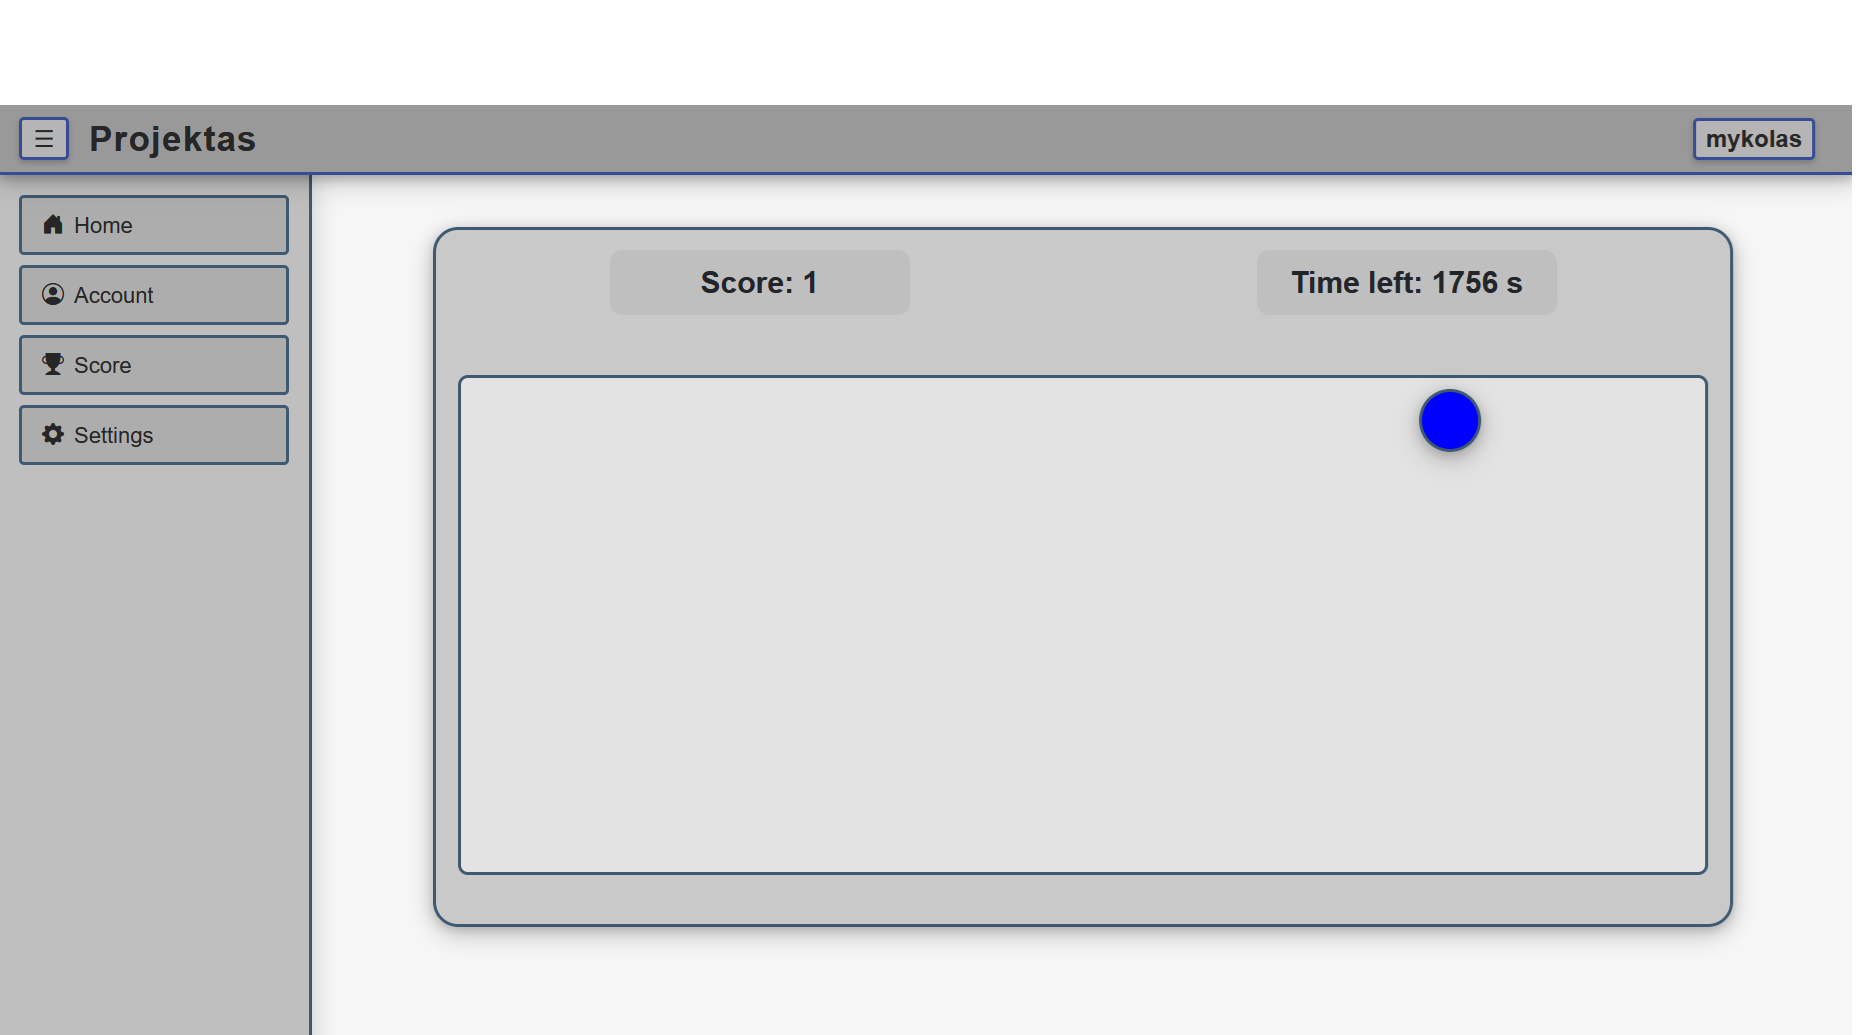
\includegraphics[width=1\textwidth,keepaspectratio]{PSI_3rd_trial/PNGs/aim_trainer_2.png}
    \caption{Aim Trainer gameplay page GUI after scoring once}
    \label{fig:aim_trainer_2}
\end{figure}

\begin{figure}[H]
    \centering
    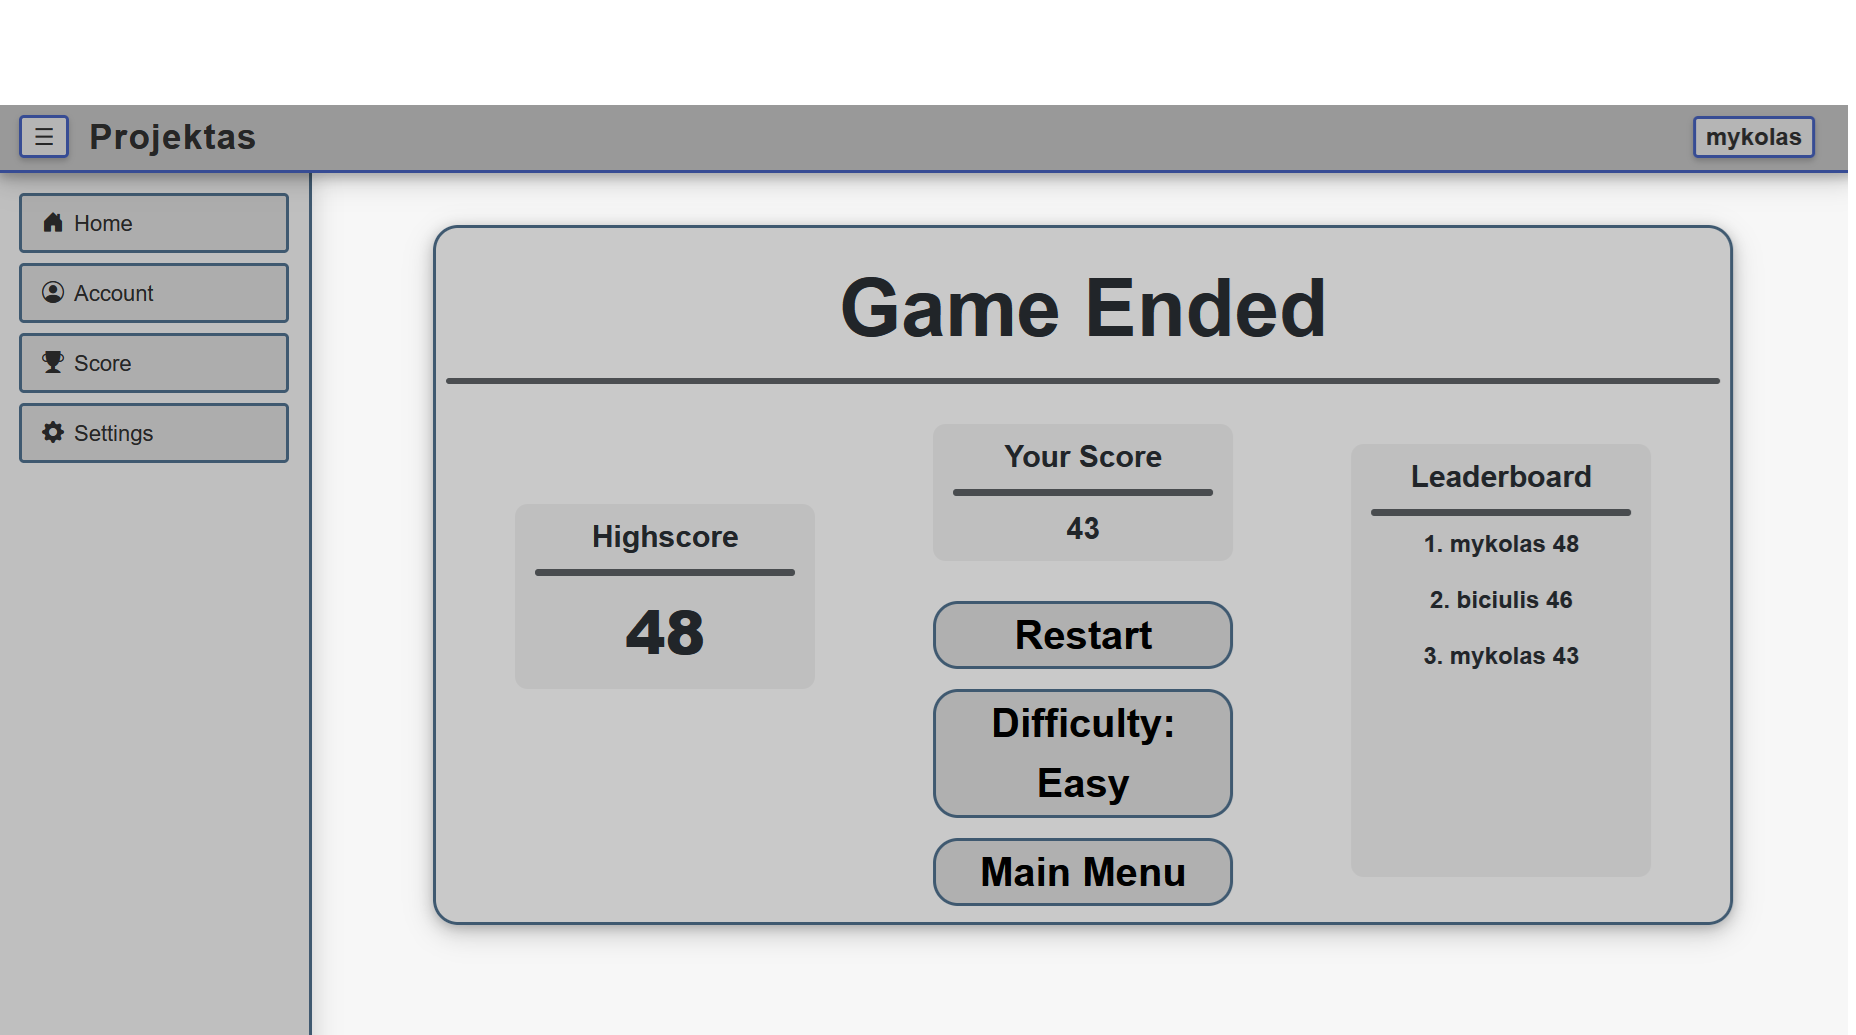
\includegraphics[width=1\textwidth,keepaspectratio]{PSI_3rd_trial/PNGs/aim_trainer_3.png}
    \caption{Aim trainer page GUI after the game ends}
    \label{fig:aim_trainer_3}
\end{figure}

\heading{Basic Course:}
The system generates a new target and initializes the Aim Trainer gameplay page. The User clicks a target. The system checks if the timer has not yet finished. The system removes the clicked target, increments the score, generates a new target and displays the Aim Trainer gameplay page with the new target. After the timer runs out, the system saves the player's score to the high score entry and displays the score of the player. 


\heading{Alternate Course(player is logged out):}
After the timer runs out, the player's score is not saved.

\begin{figure}[H]
    \centering
    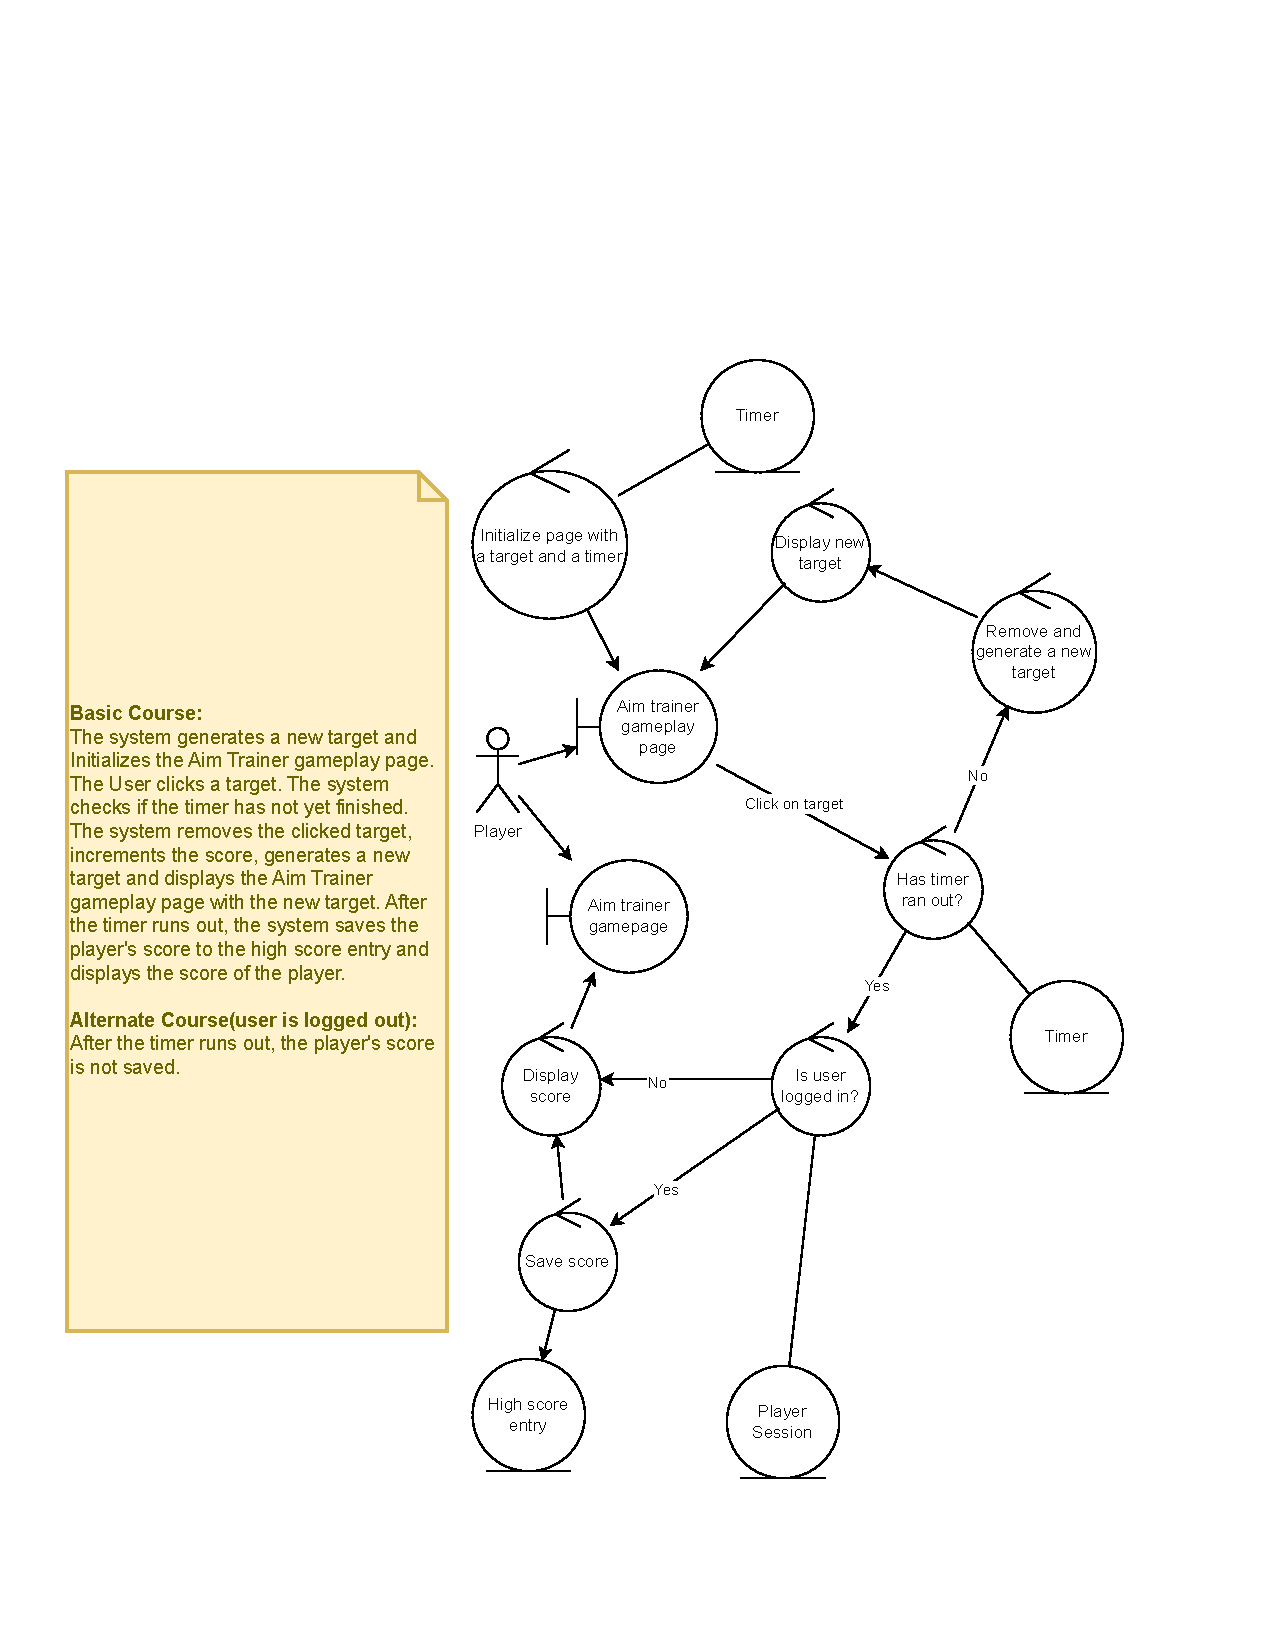
\includegraphics[width=1\textwidth,keepaspectratio]{PSI_3rd_trial/robustness/aim_trainer.drawio.pdf}
    \caption{Aim Trainer Robustness diagram}
    \label{fig:aim_trainer_diagram}
\end{figure}

This use case is derived from the Functional Requirements 2.d., 3.c., 3.d., 3.f. 3.g.

\subsubsection{Play Sudoku}

\begin{figure}[H]
    \centering
    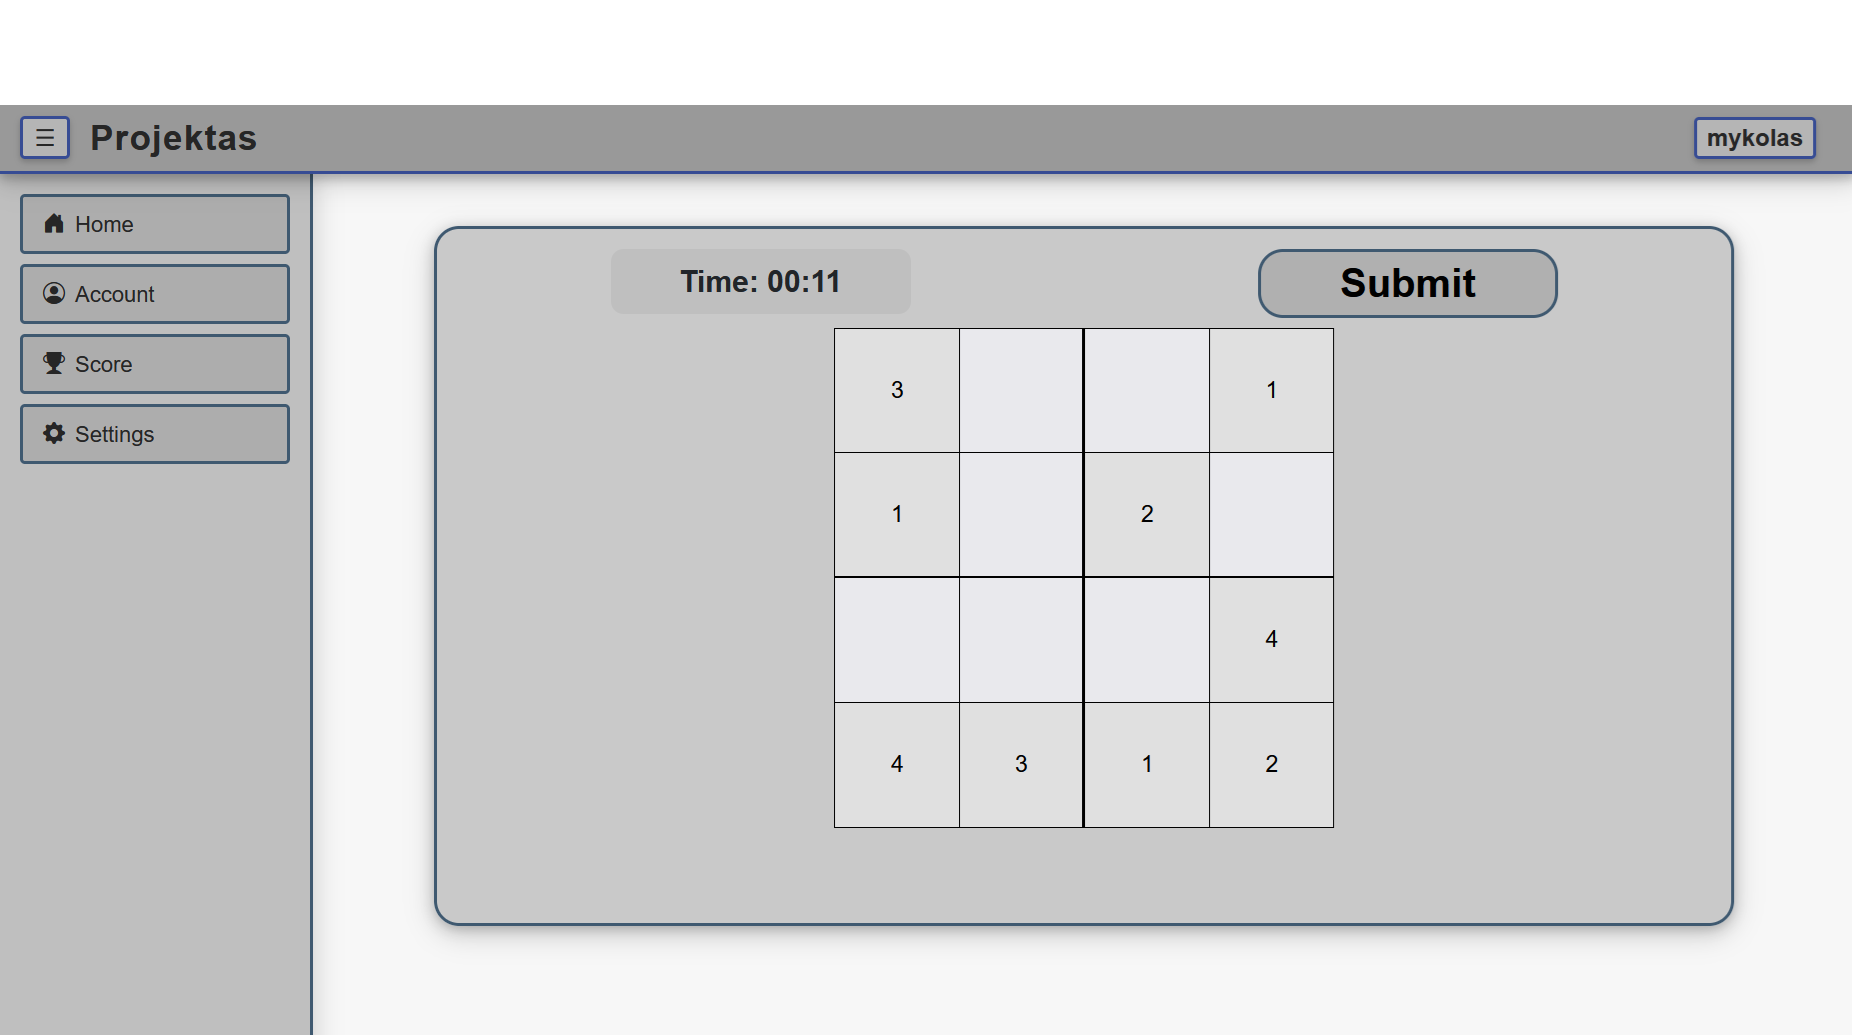
\includegraphics[width=1\textwidth,keepaspectratio]{PSI_3rd_trial/PNGs/sudoku_1.png}
    \caption{Sudoku gameplay page initial GUI}
    \label{fig:sudoku_1}
\end{figure}


\begin{figure}[H]
    \centering
    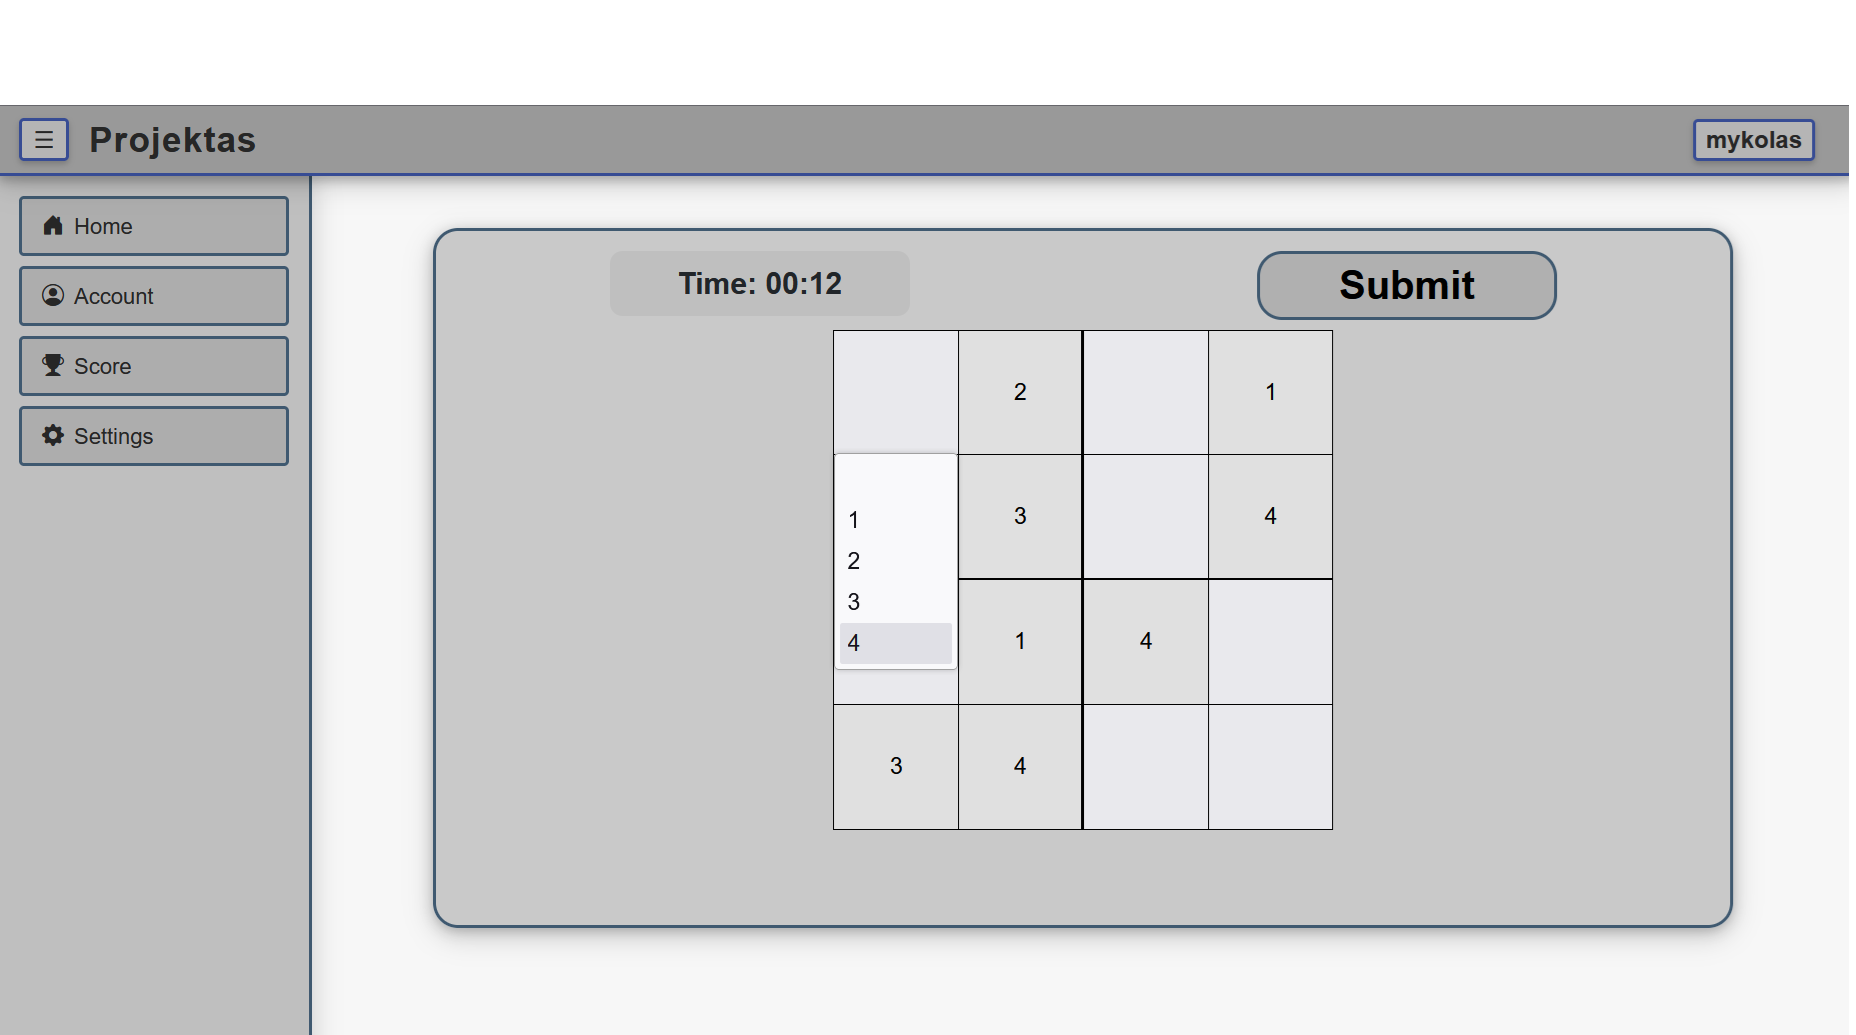
\includegraphics[width=1\textwidth,keepaspectratio]{PSI_3rd_trial/PNGs/sudoku_4.png}
    \caption{Sudoku gameplay page GUI with a cell selected}
    \label{fig:sudoku_4}
\end{figure}


\begin{figure}[H]
    \centering
    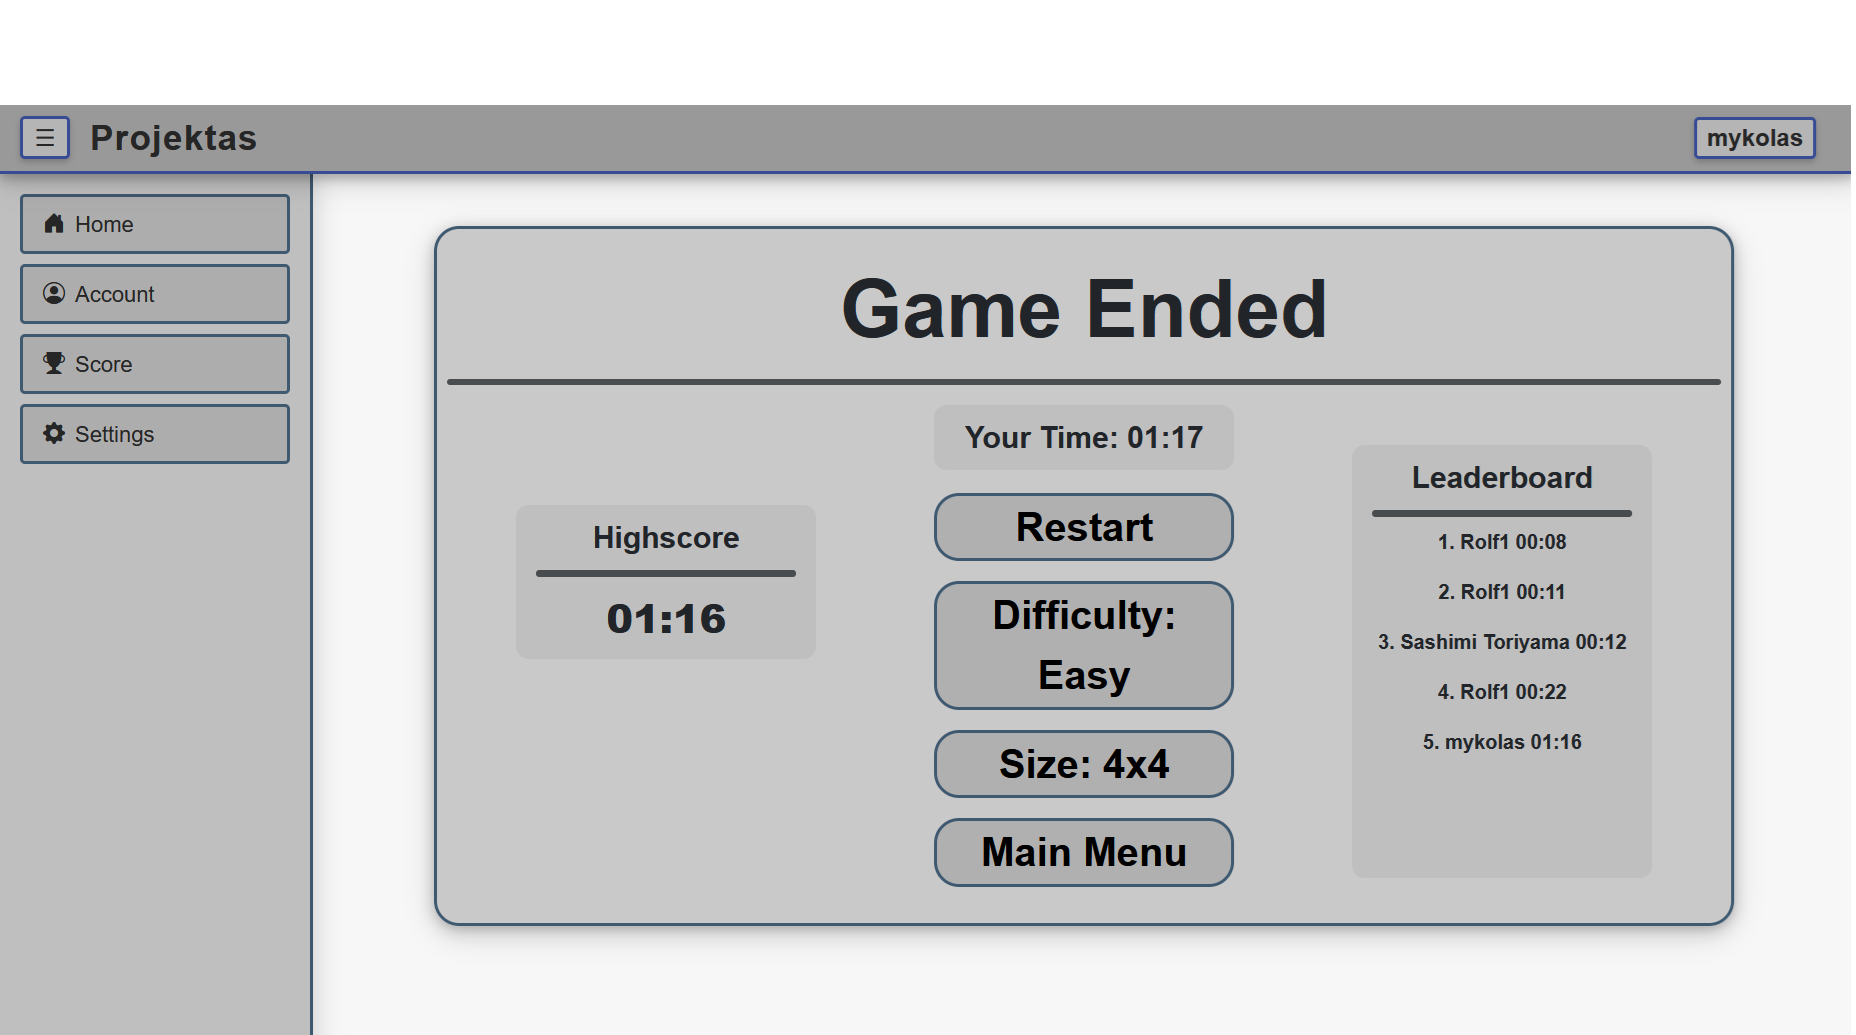
\includegraphics[width=1\textwidth,keepaspectratio]{PSI_3rd_trial/PNGs/sudoku_3.png}
    \caption{Sudoku page GUI after the game has ended}
    \label{fig:sudoku_3}
\end{figure}

% Include the detail that a score is displayed after the game ends. 3.f.
% Include the detail that the leaderboards get updated after a player with an account finishes a game. 3.g.

\heading{Basic Course:}
The system initializes the Sudoku gameplay page with a Sudoku table and a timer. Player enters their solution and clicks submit answer. The system checks if the submitted board is correct. The system saves the score and displays the Sudoku page with the final score.

\heading{Alternate Course (the board was incorrect):}
The system displays the Sudoku gameplay page with the message "incorrect solution".

\heading{Alternate Course (the player is logged out):}
The system does not save the player's score.

\begin{figure}[H]
    \centering
    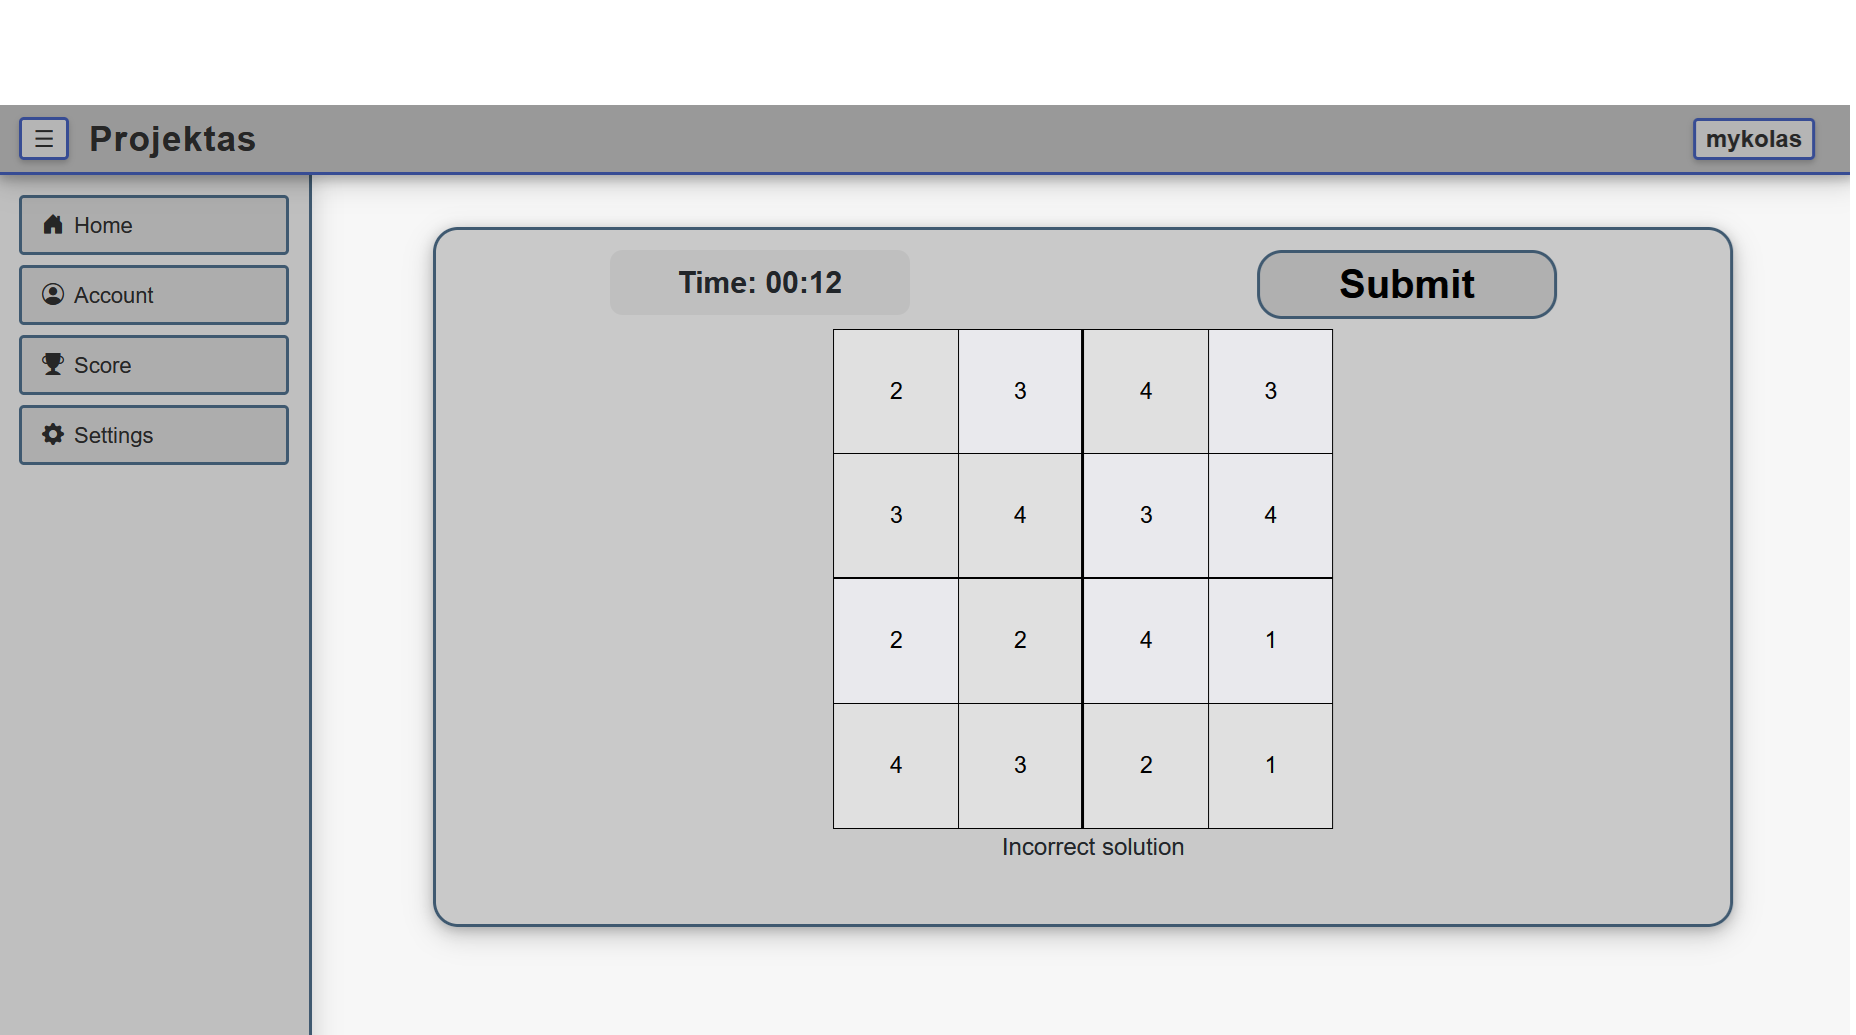
\includegraphics[width=1\textwidth,keepaspectratio]{PSI_3rd_trial/PNGs/sudoku_2.png}
    \caption{Sudoku gameplay page GUI after an incorrect solution was submitted}
    \label{fig:sudoku_2}
\end{figure}

\heading{Alternate Course (the player is logged out):}
The system does not save the player's score.

\begin{figure}[H]
    \centering
    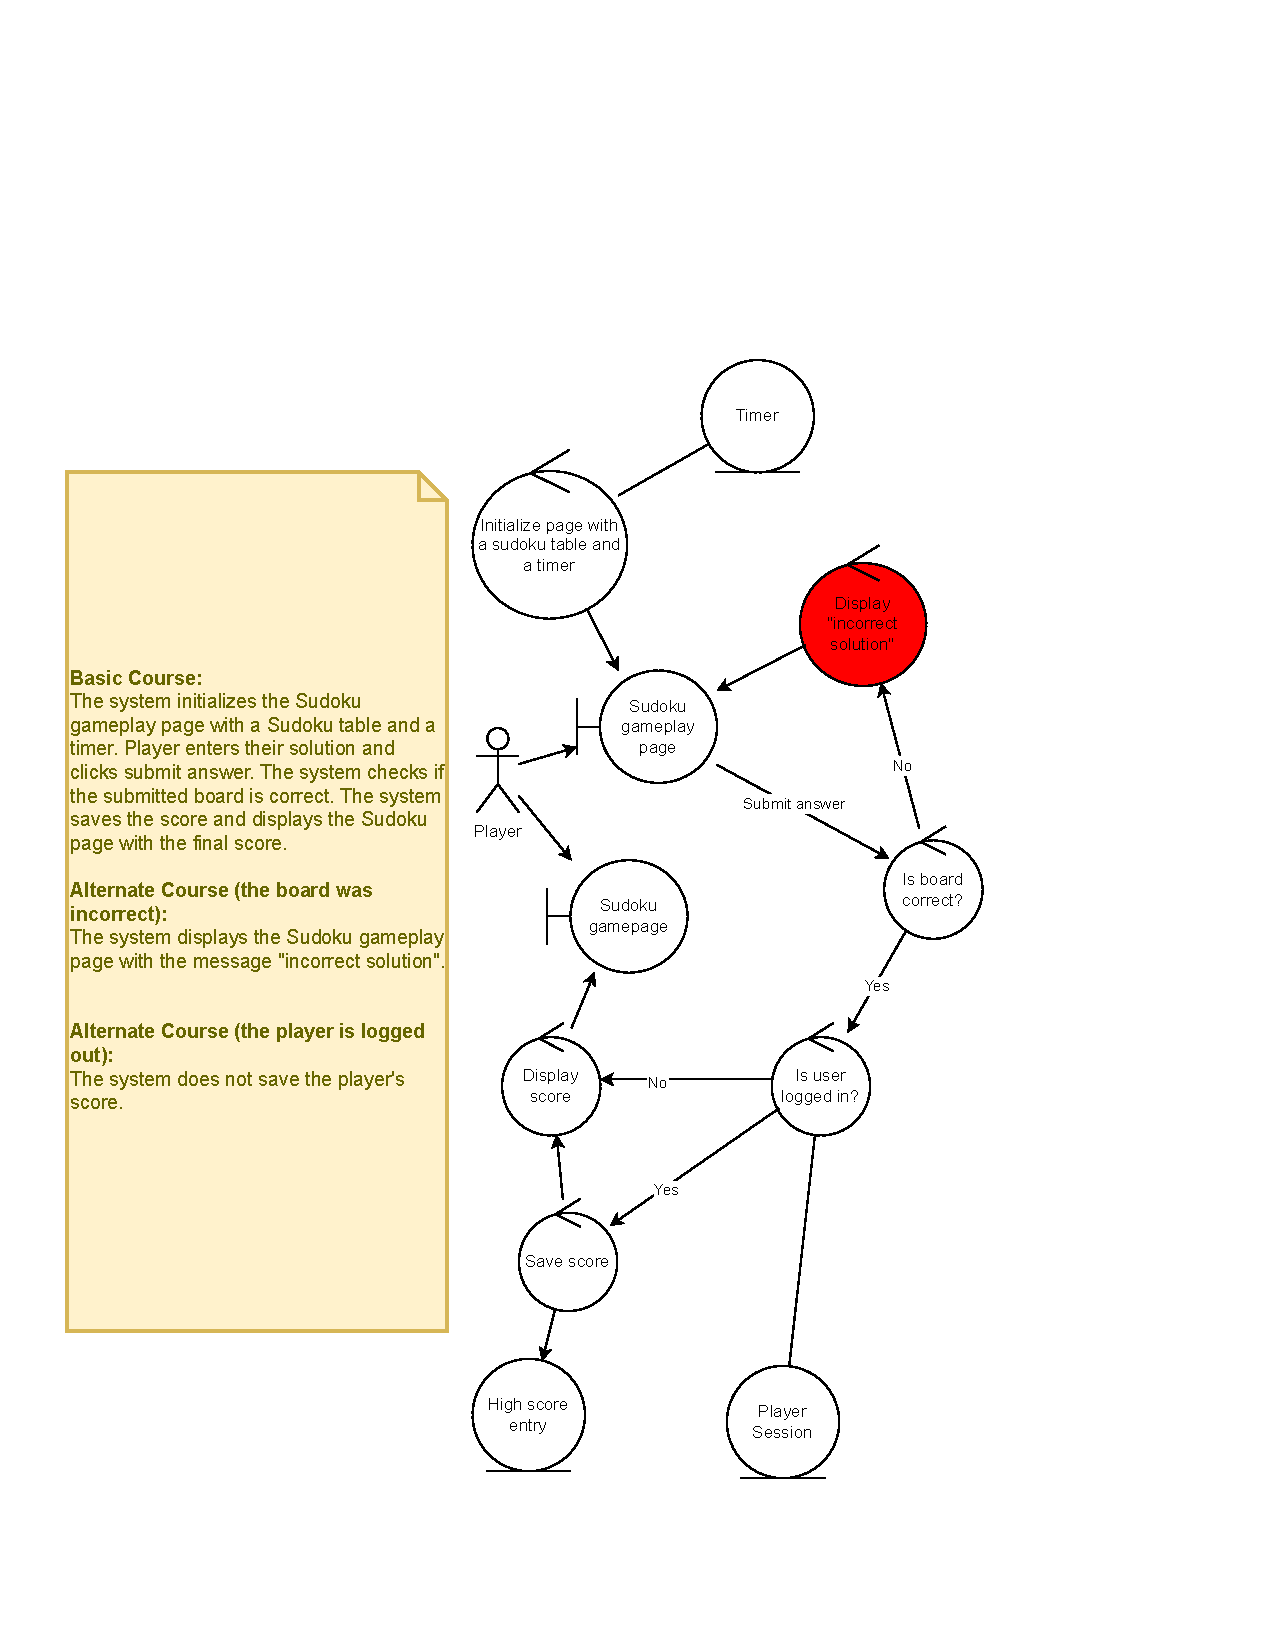
\includegraphics[width=1\textwidth,keepaspectratio]{PSI_3rd_trial/robustness/sudoku.drawio.pdf}
    \caption{Sudoku Robustness Diagram}
    \label{fig:sudoku_diagram}
\end{figure}


This use case is derived from the Functional Requirements 2.c., 3.c., 3.d., 3.f. 3.g.

\subsubsection{Play Math Game}

% Include the detail that a score is displayed after the game ends. 3.f.
% Include the detail that the leaderboards get updated after a player with an account finishes a game. 3.g.
\begin{figure}[H]
    \centering
    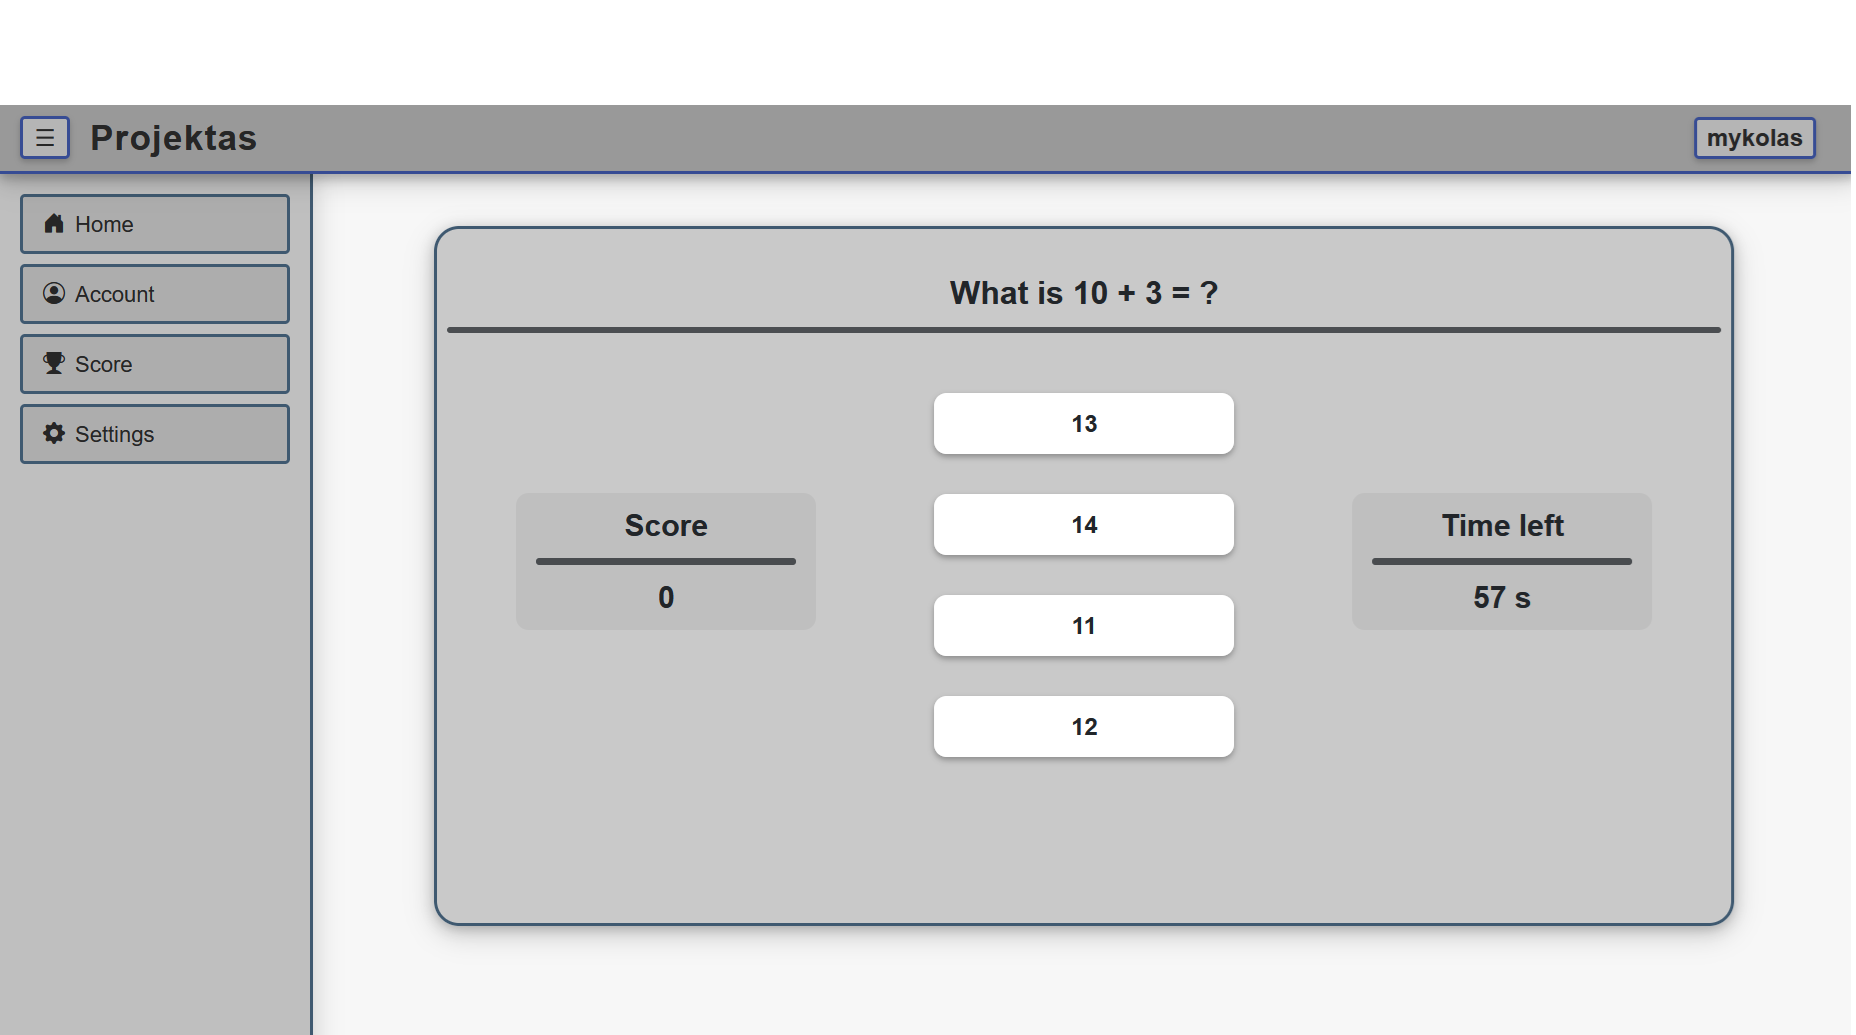
\includegraphics[width=1\textwidth,keepaspectratio]{PSI_3rd_trial/PNGs/math_game_1.png}
    \caption{Math gameplay page initial GUI}
    \label{fig:math_game_1}
\end{figure}


\begin{figure}[H]
    \centering
    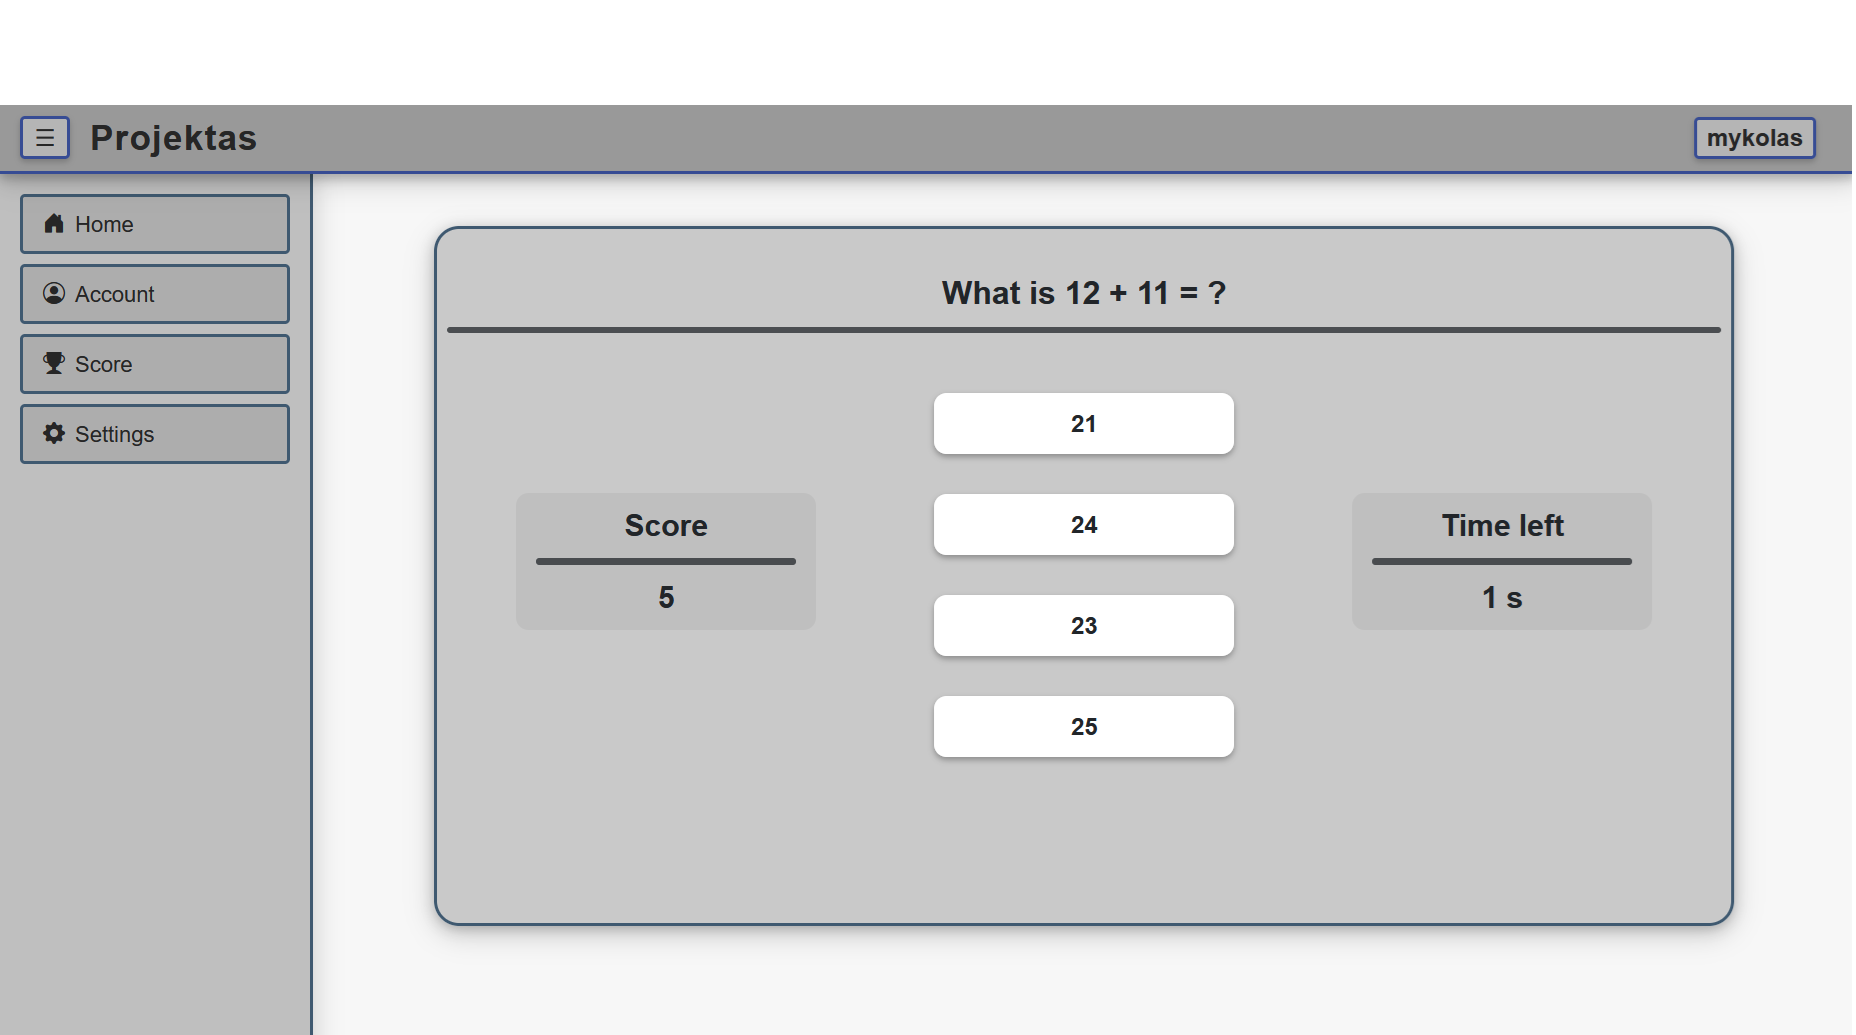
\includegraphics[width=1\textwidth,keepaspectratio]{PSI_3rd_trial/PNGs/math_game_2.png}
    \caption{Math gameplay page GUI after answering 5 questions correctly}
    \label{fig:math_game_2}
\end{figure}

\begin{figure}[H]
    \centering
    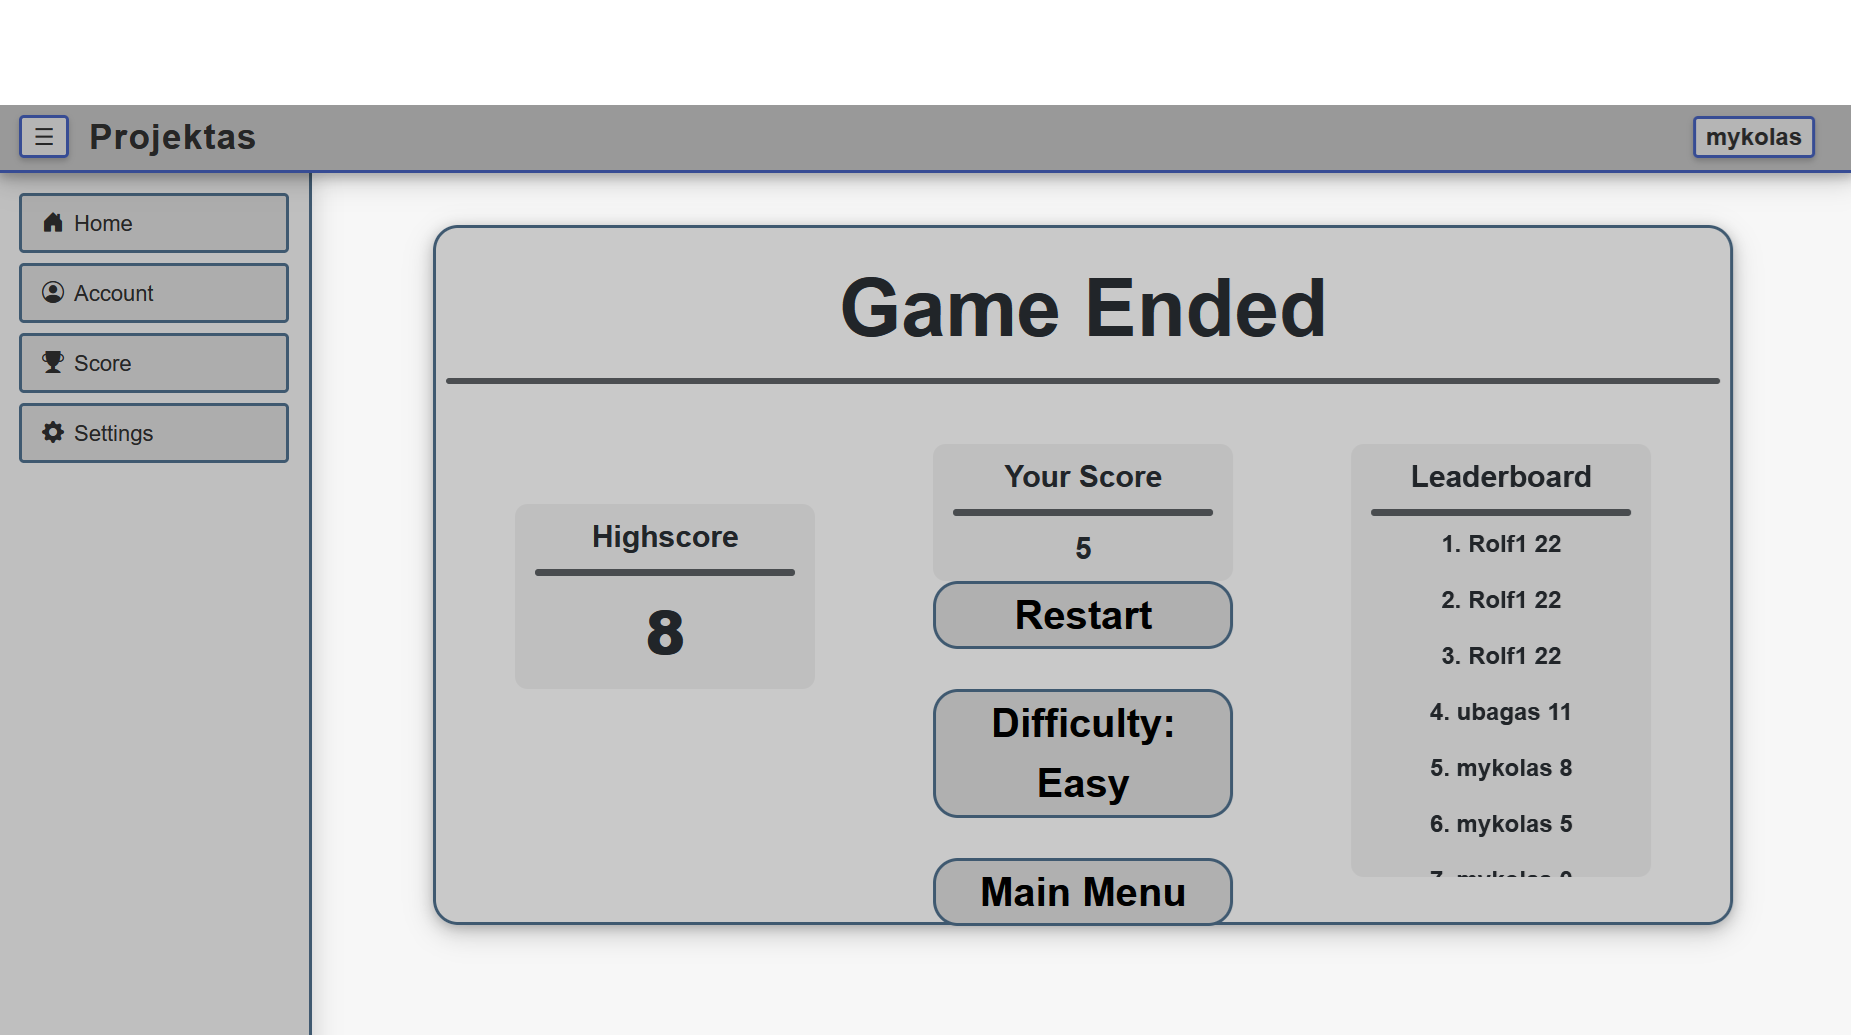
\includegraphics[width=1\textwidth,keepaspectratio]{PSI_3rd_trial/PNGs/math_game_3.png}
    \caption{Math game page GUI after the game has ended}
    \label{fig:math_game_3}
\end{figure}

\heading{Basic Course:}
The system displays the Math Game page with generated question, answer choices and timer. The system generates a math question and answer options on the gameplay page. The player selects an answer. The system verifies if the timer has not expired. The system checks if the selected answer is correct. The system increments the score, generates a new math question with answer options. The system detects that the timer has expired. The system ignores the selection and updates the gameplay page to display the final score.

\heading{Alternate Course (Incorrect Answer):}
The system does not change the score.

\heading{Alternate Course (Player is not logged in):}
The system does not save the score.

\begin{figure}[H]
    \centering
    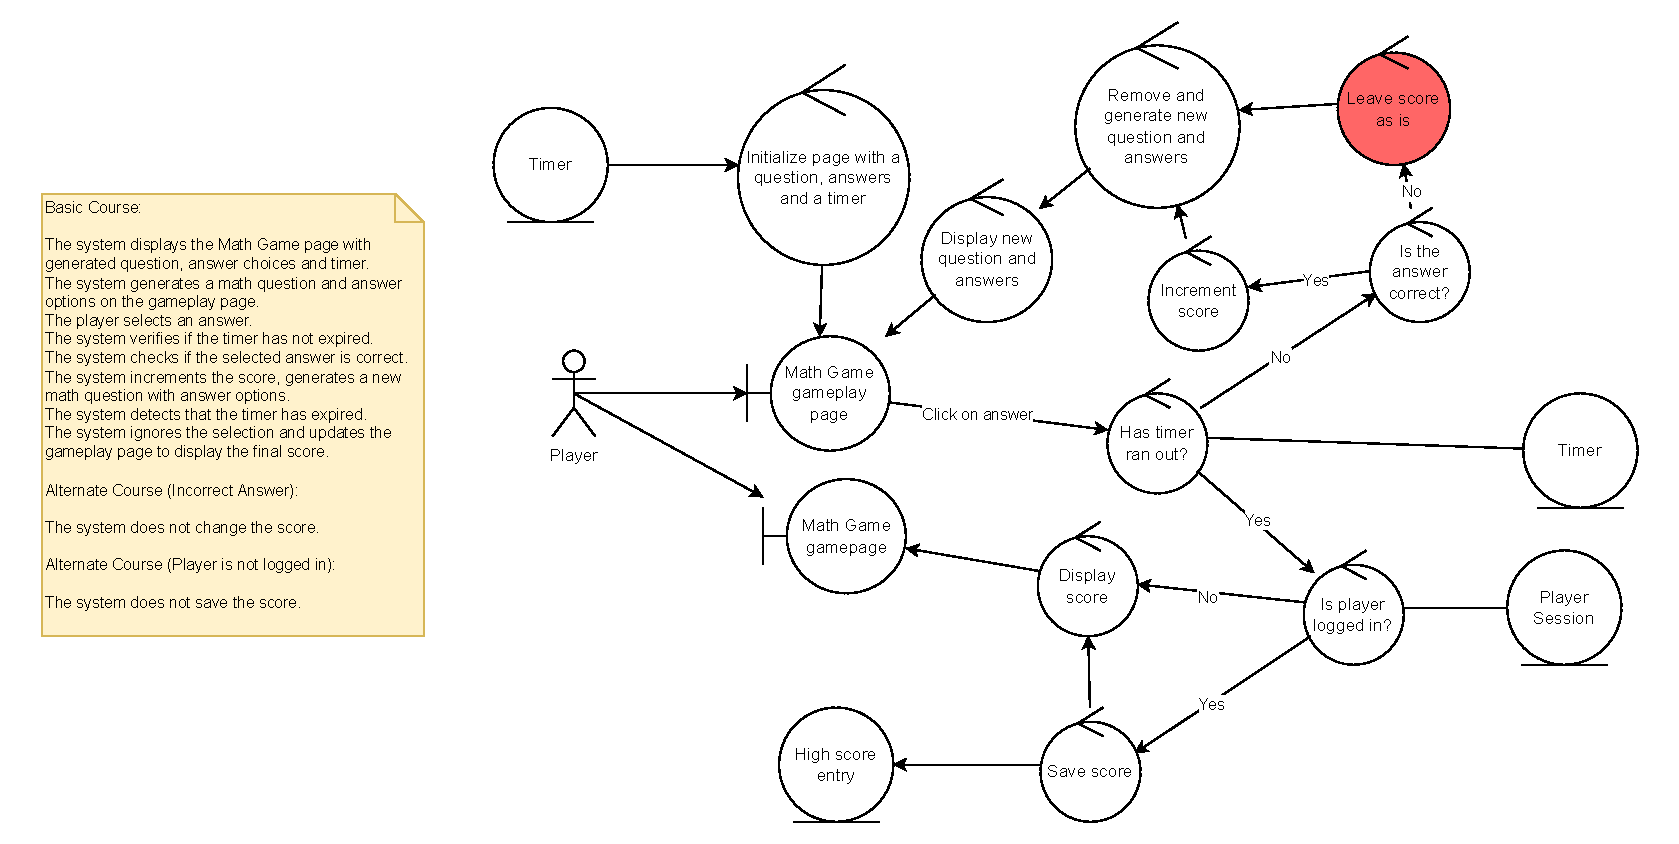
\includegraphics[width=1\textwidth,keepaspectratio]{PSI_3rd_trial/robustness/math_game.drawio-1.pdf}
    \caption{Play Math Game Robustness Diagram}
    \label{fig:math_game_robustness_diagram}
\end{figure}

This use case is derived from the Functional Requirements 2.a., 3.c., 3.d., 3.f., 3.g.

\subsection{Statistics package}

\begin{figure}[H]
    \centering
    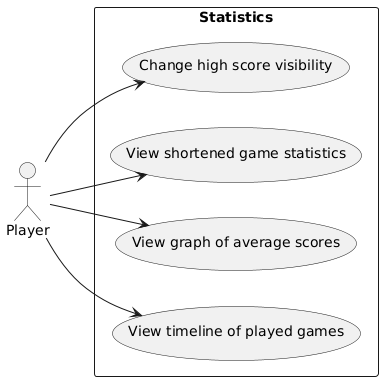
\includegraphics[keepaspectratio]{PSI_3rd_trial/use_case_high_score.png}
    \caption{Statistics use case package diagram}
    \label{fig:statistics_package}
\end{figure}

\subsubsection{Change high score visibility}

\begin{figure}[H]
    \centering
    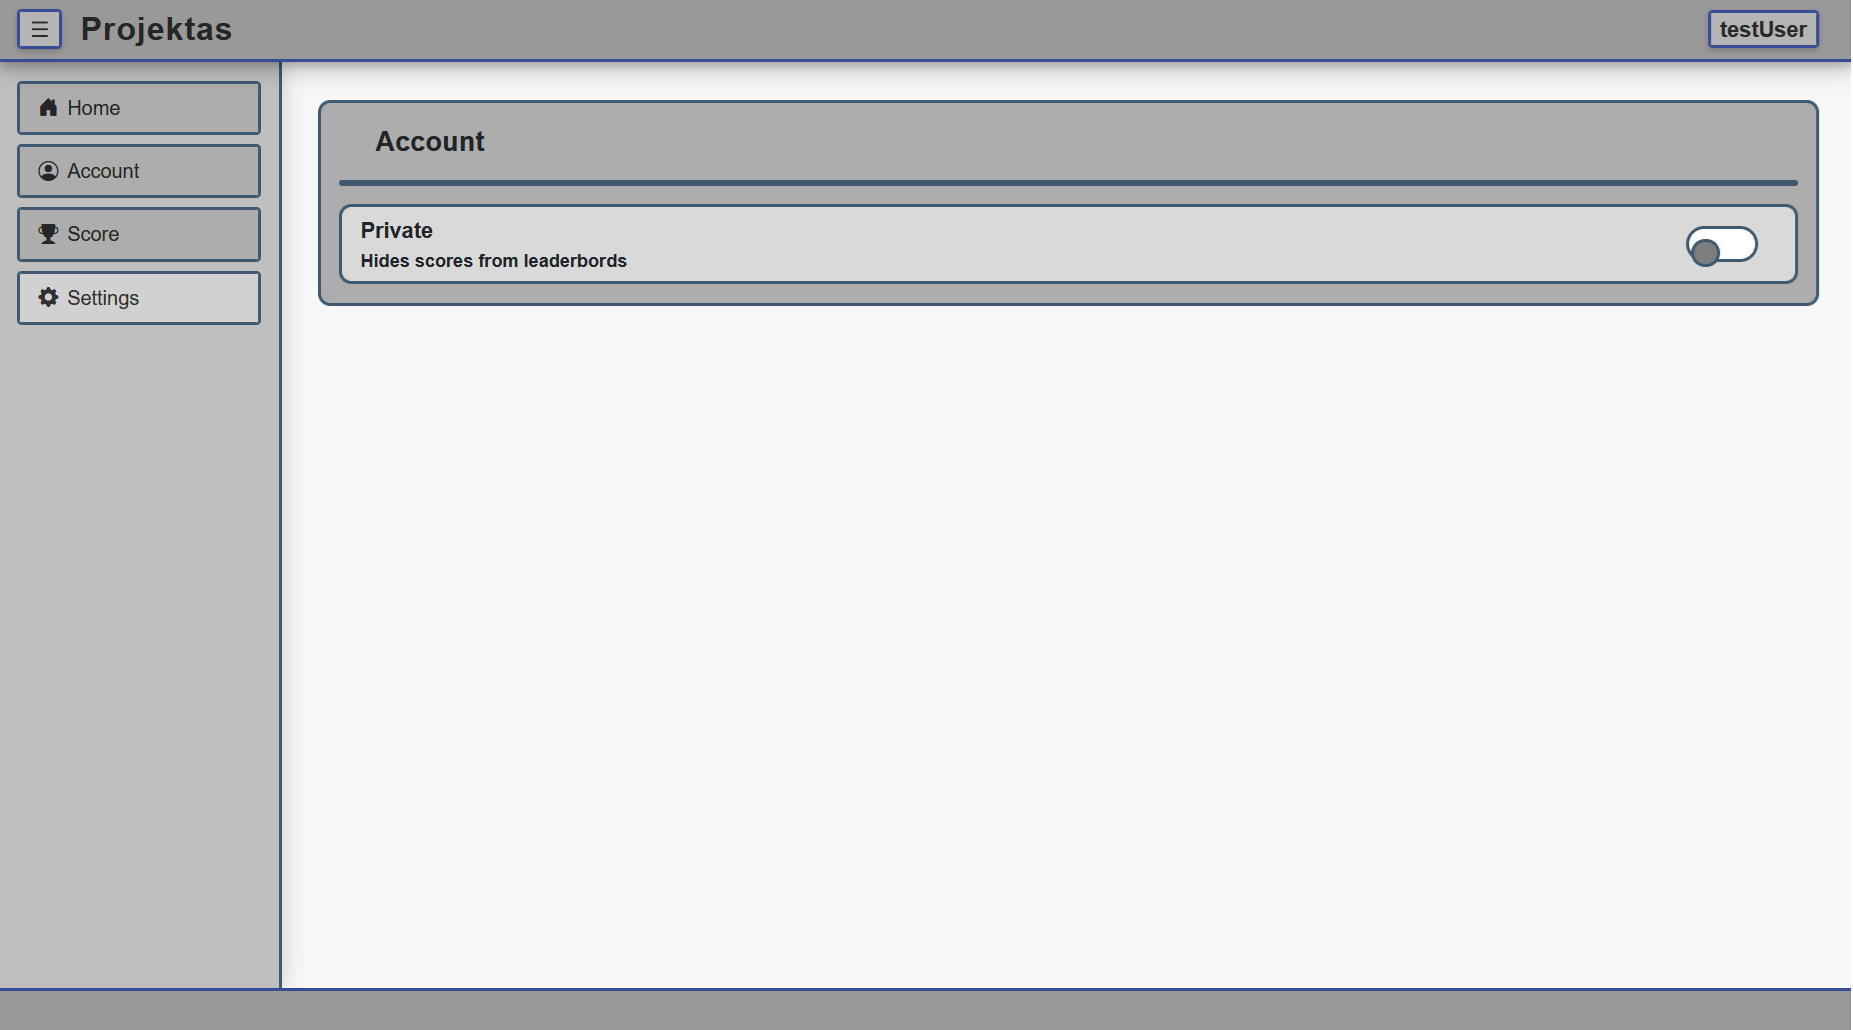
\includegraphics[width=1\textwidth,keepaspectratio]{PSI_3rd_trial/PNGs/privacy_settings_off.png}
    \caption{Privacy setting is off}
    \label{fig:privacy_settings_off}
\end{figure}

\begin{figure}[H]
    \centering
    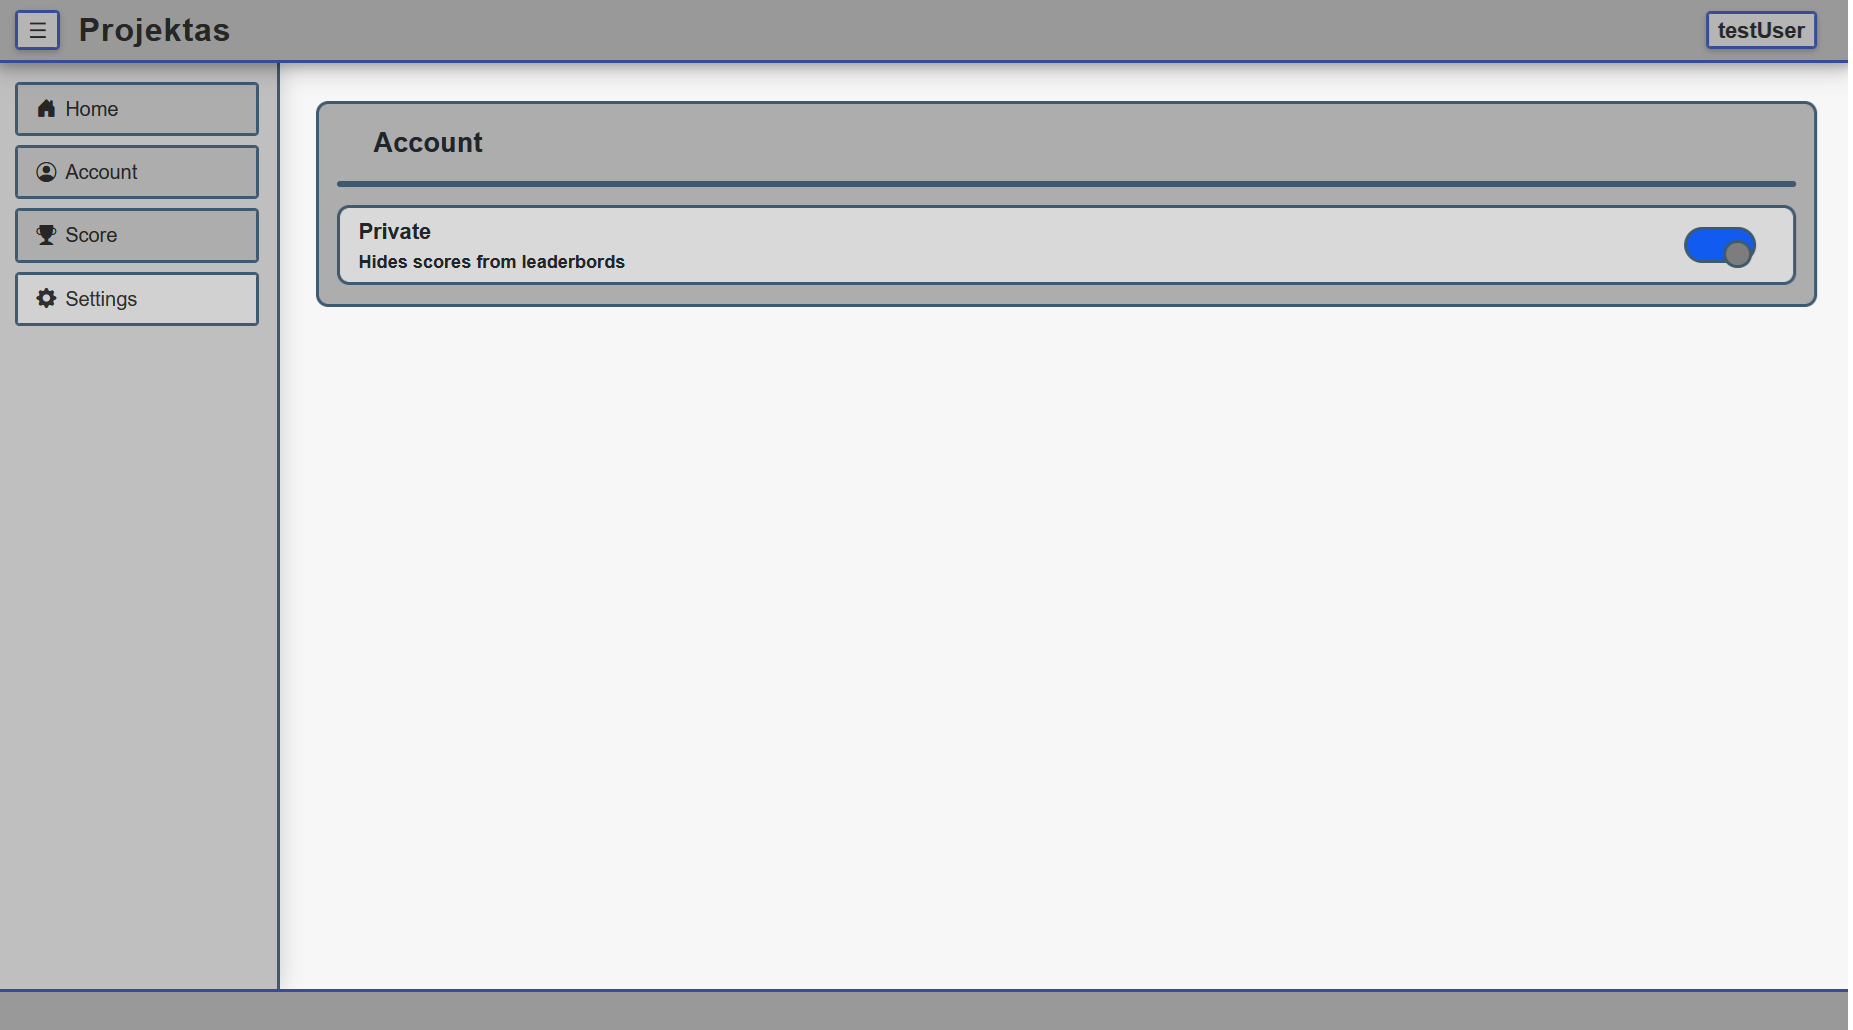
\includegraphics[width=1\textwidth,keepaspectratio]{PSI_3rd_trial/PNGs/privacy_settings_on.png}
    \caption{Privacy setting is on}
    \label{fig:privacy_settings_on}
\end{figure}


\heading{Basic Course:}
The system displays the settings page. The player clicks the privacy switch bar. The system checks if the privacy switch is active. The system marks the player’s scores as private and hides them in the leaderboards. The system activates the switch.

\heading{Alternate Course (The scores were already private):}
The system marks the player’s scores as public and reveals them in the leaderboards. The system deactivates the switch.

\begin{figure}[H]
    \centering
    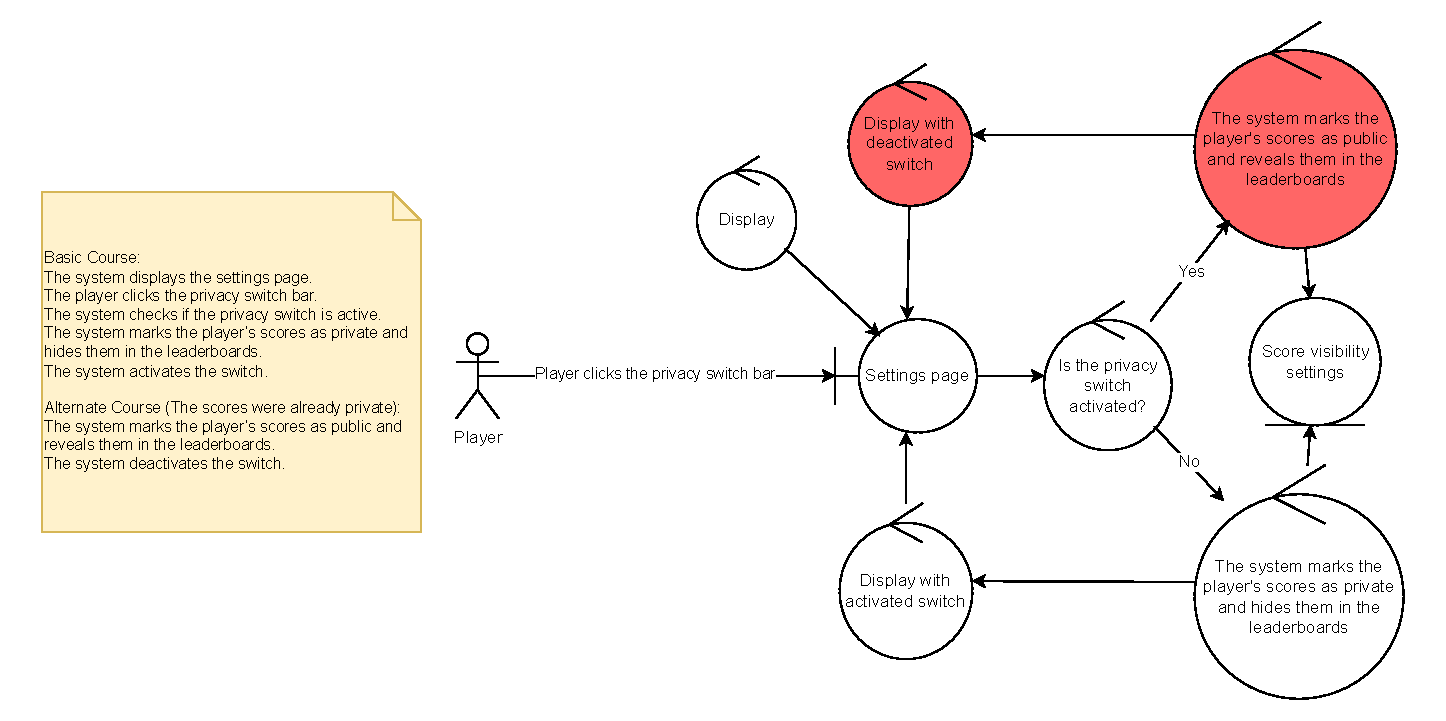
\includegraphics[width=1\textwidth,keepaspectratio]{PSI_3rd_trial/robustness/score_privacy.drawio.pdf}
    \caption{Change High Score Visibility Robustness Diagram}
    \label{fig:high_score_visibility_diagram}
\end{figure}

This use case is derived from the Functional Requirements 1.c, 3.e.

\subsubsection{View shortened game statistics}

\begin{figure}[H]
    \centering
    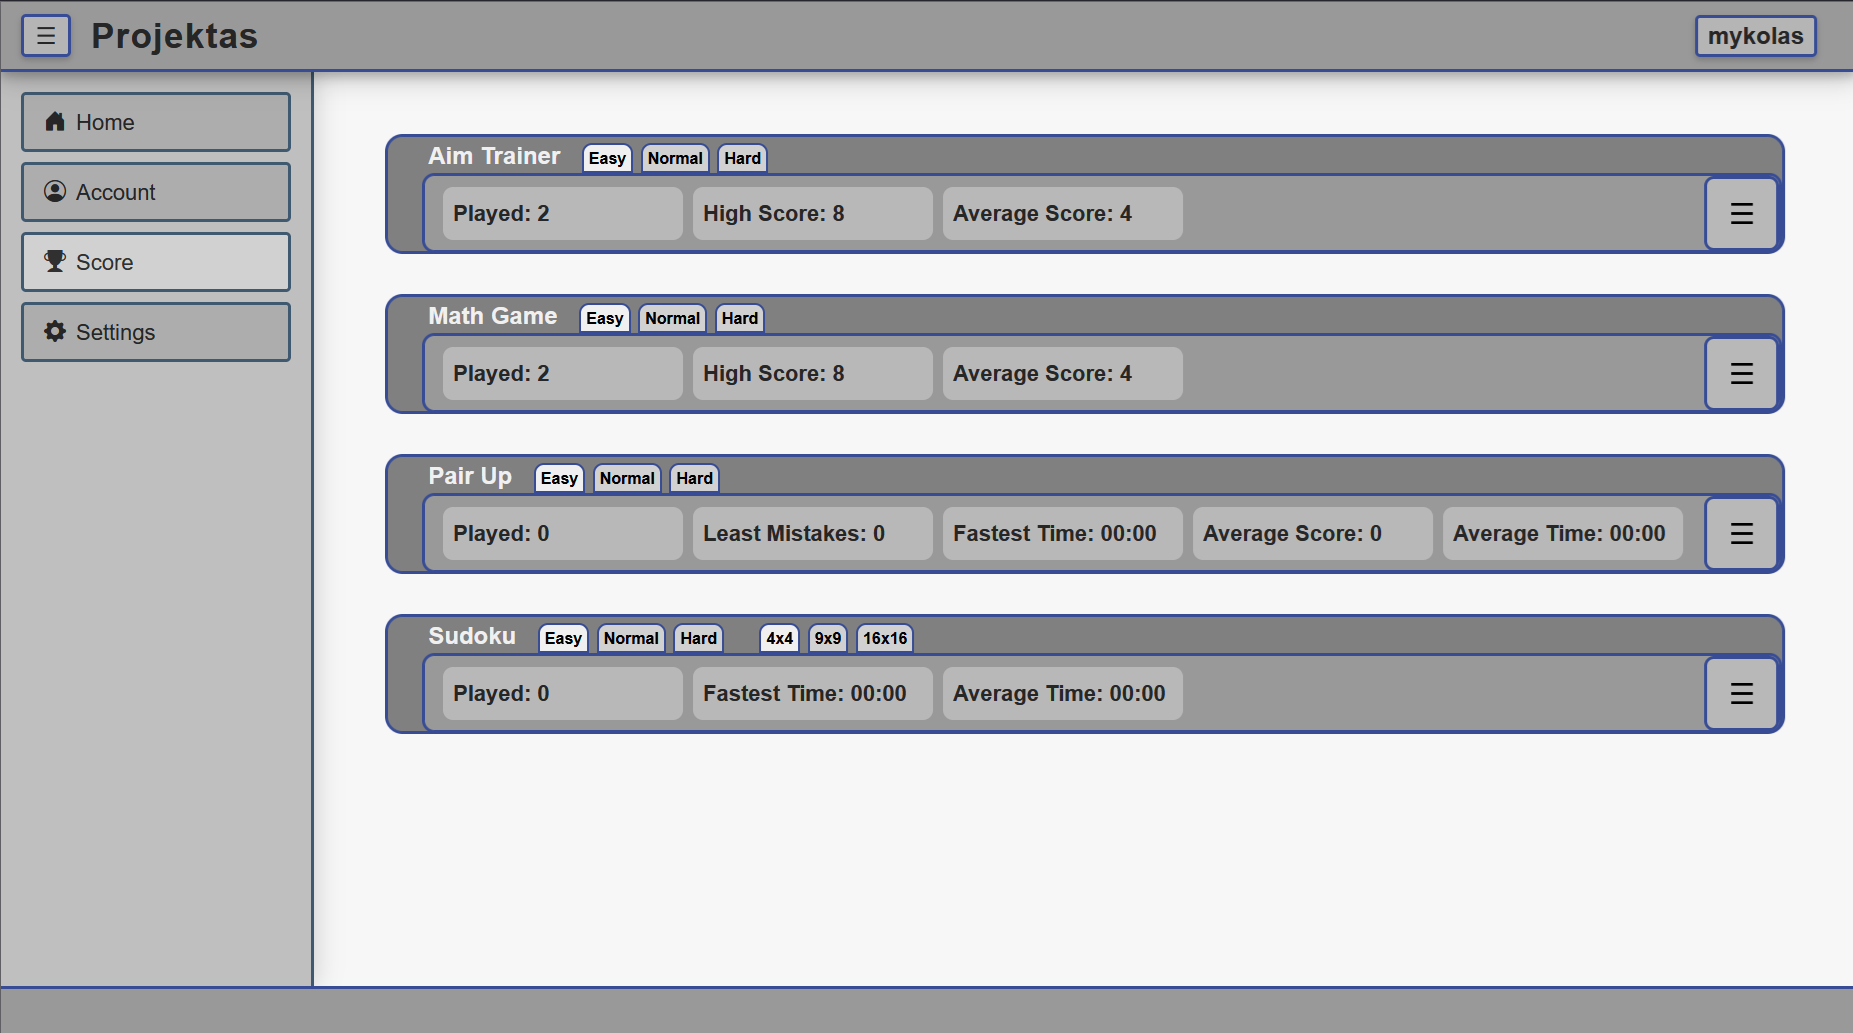
\includegraphics[width=1\textwidth,keepaspectratio]{PSI_3rd_trial/PNGs/score_page.png}
    \caption{Statistics page GUI}
    \label{fig:score_page}
\end{figure}


\heading{Basic Course:}
The system checks if the player is logged in. The system displays the statistics page. The player selects the difficulty with the buttons near a specific game. The system checks if personal statistics are available. The system displays a shortened version of the statistics (amount of games played, highest score, average score) for that game filtered by the selected difficulty. The player views the shortened game statistics.

\heading{Alternate Course (No Scores Were Found):}
The system shows a message indicating that no scores were found.

\heading{Alternate Course (Player is not logged in):}
The system shows a create an account message.

\begin{figure}[H]
    \centering
    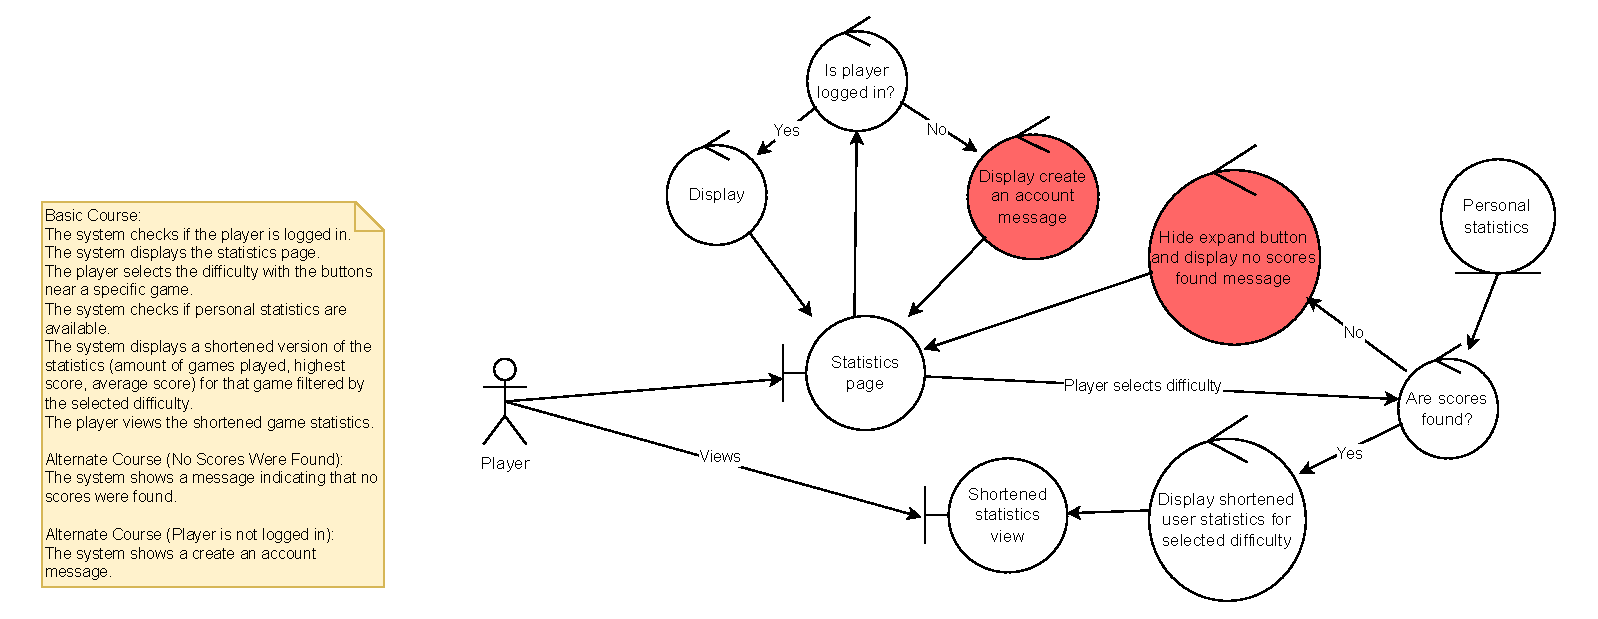
\includegraphics[width=1\textwidth,keepaspectratio]{PSI_3rd_trial/robustness/short_stats.drawio.pdf}
    \caption{View Shortened Game Statistics Robustness Diagram}
    \label{fig:shortened_statistics_view_diagram}
\end{figure}

This use case is derived from the Functional Requirements 1.e, 3.e.


\subsubsection{View graph of average scores}


\heading{Basic Course:}
The system checks if the player is logged in. The system displays the statistics page. The player clicks the expand button near a
game. The system displays the expanded statistics
view. The player clicks the "average score" button. The system checks if personal statistics are available. The system displays a graph view of the player's average score for the last 7 days (for all difficulties). The user views the graph.

\heading{Alternate Course (No Scores Were Found):}
The system hides the expand button and shows a message indicating that no scores were found.

\heading{Alternate Course (Player is not logged in):}
The system shows a create an account message.

\begin{figure}[H]
    \centering
    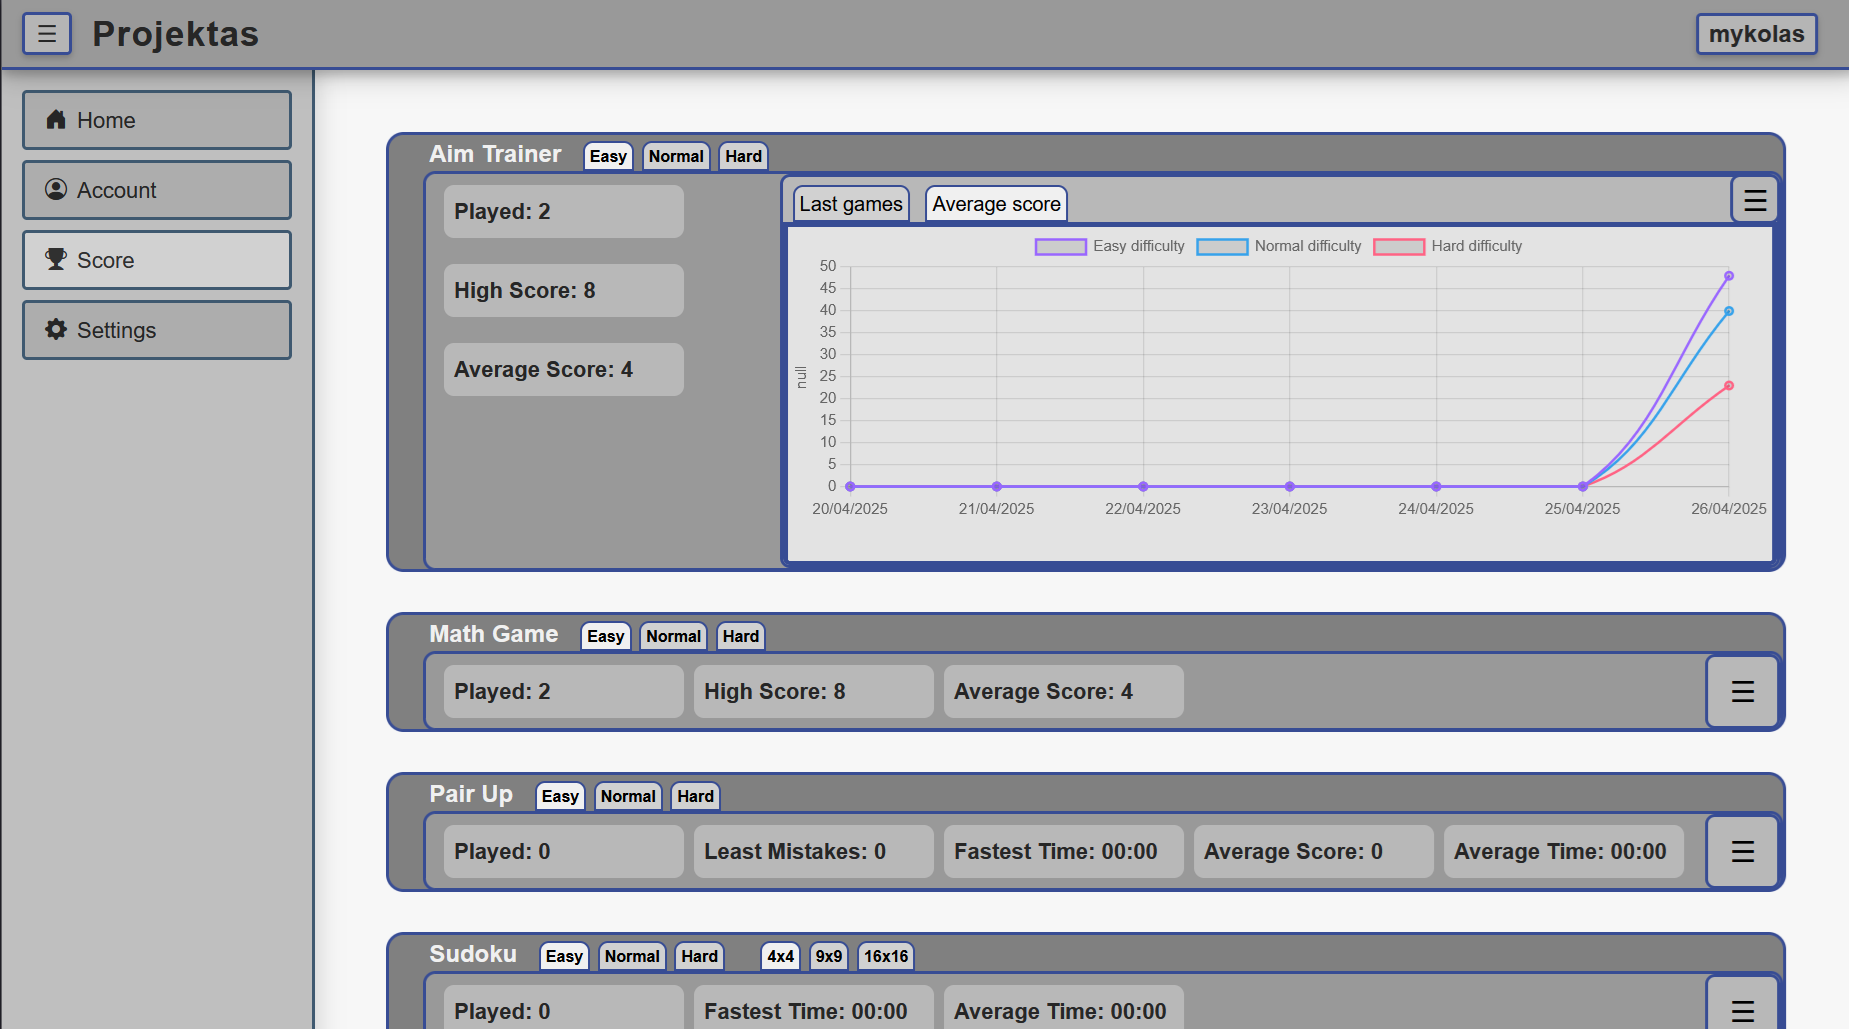
\includegraphics[width=1\textwidth,keepaspectratio]{PSI_3rd_trial/PNGs/graph_of_average_scores.png}
    \caption{Graph on the score page}
    \label{fig:graph_of_average_scores}
\end{figure}

\begin{figure}[H]
    \centering
    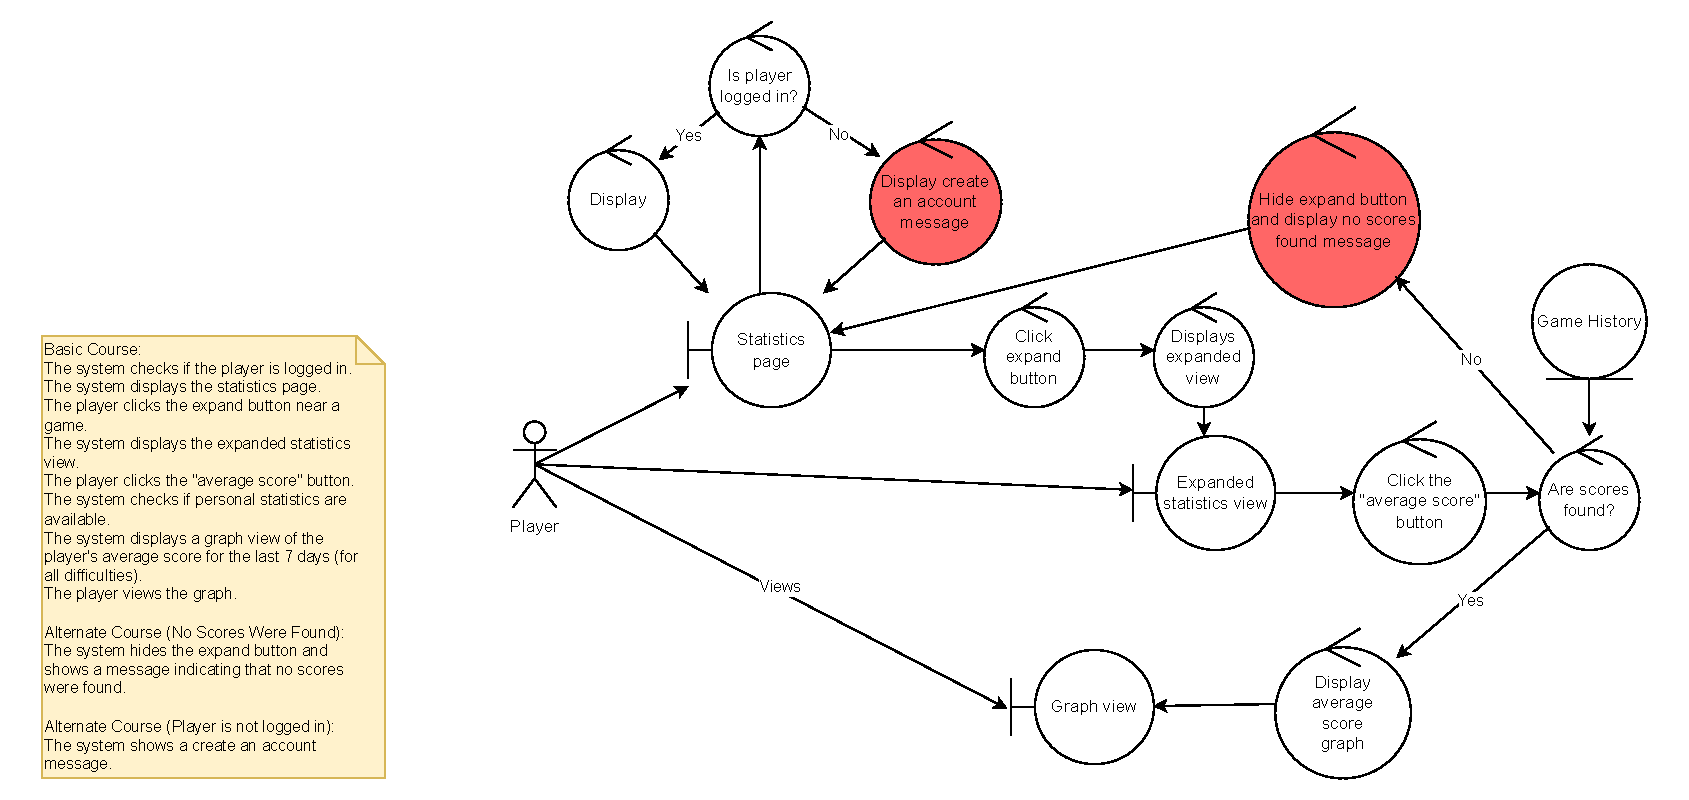
\includegraphics[width=1\textwidth,keepaspectratio]{PSI_3rd_trial/robustness/graph_stats.drawio.pdf}
    \caption{View Graph of Average Scores Robustness Diagram}
    \label{fig:average_statistics_view_diagram}
\end{figure}

This use case is derived from the Functional Requirements 1.d, 3.e.

\subsubsection{View timeline of played games}


\heading{Basic Course:}
The system checks if the player is logged in. The system displays the statistics page. The player clicks the expand button. The system displays the expanded statistics page. The player clicks the "last games" button. The system checks if game history is available. The system displays a list of the player’s 10 most recent game statistics (date, score, difficulty) for all difficulties. The player views the list of scores.

\heading{Alternate Course (No Scores Were Found):}
The system hides the expand button and shows a message indicating that no scores were found.

\heading{Alternate Course (Player is not logged in):}
The system shows a create an account message.

\begin{figure}[H]
    \centering
    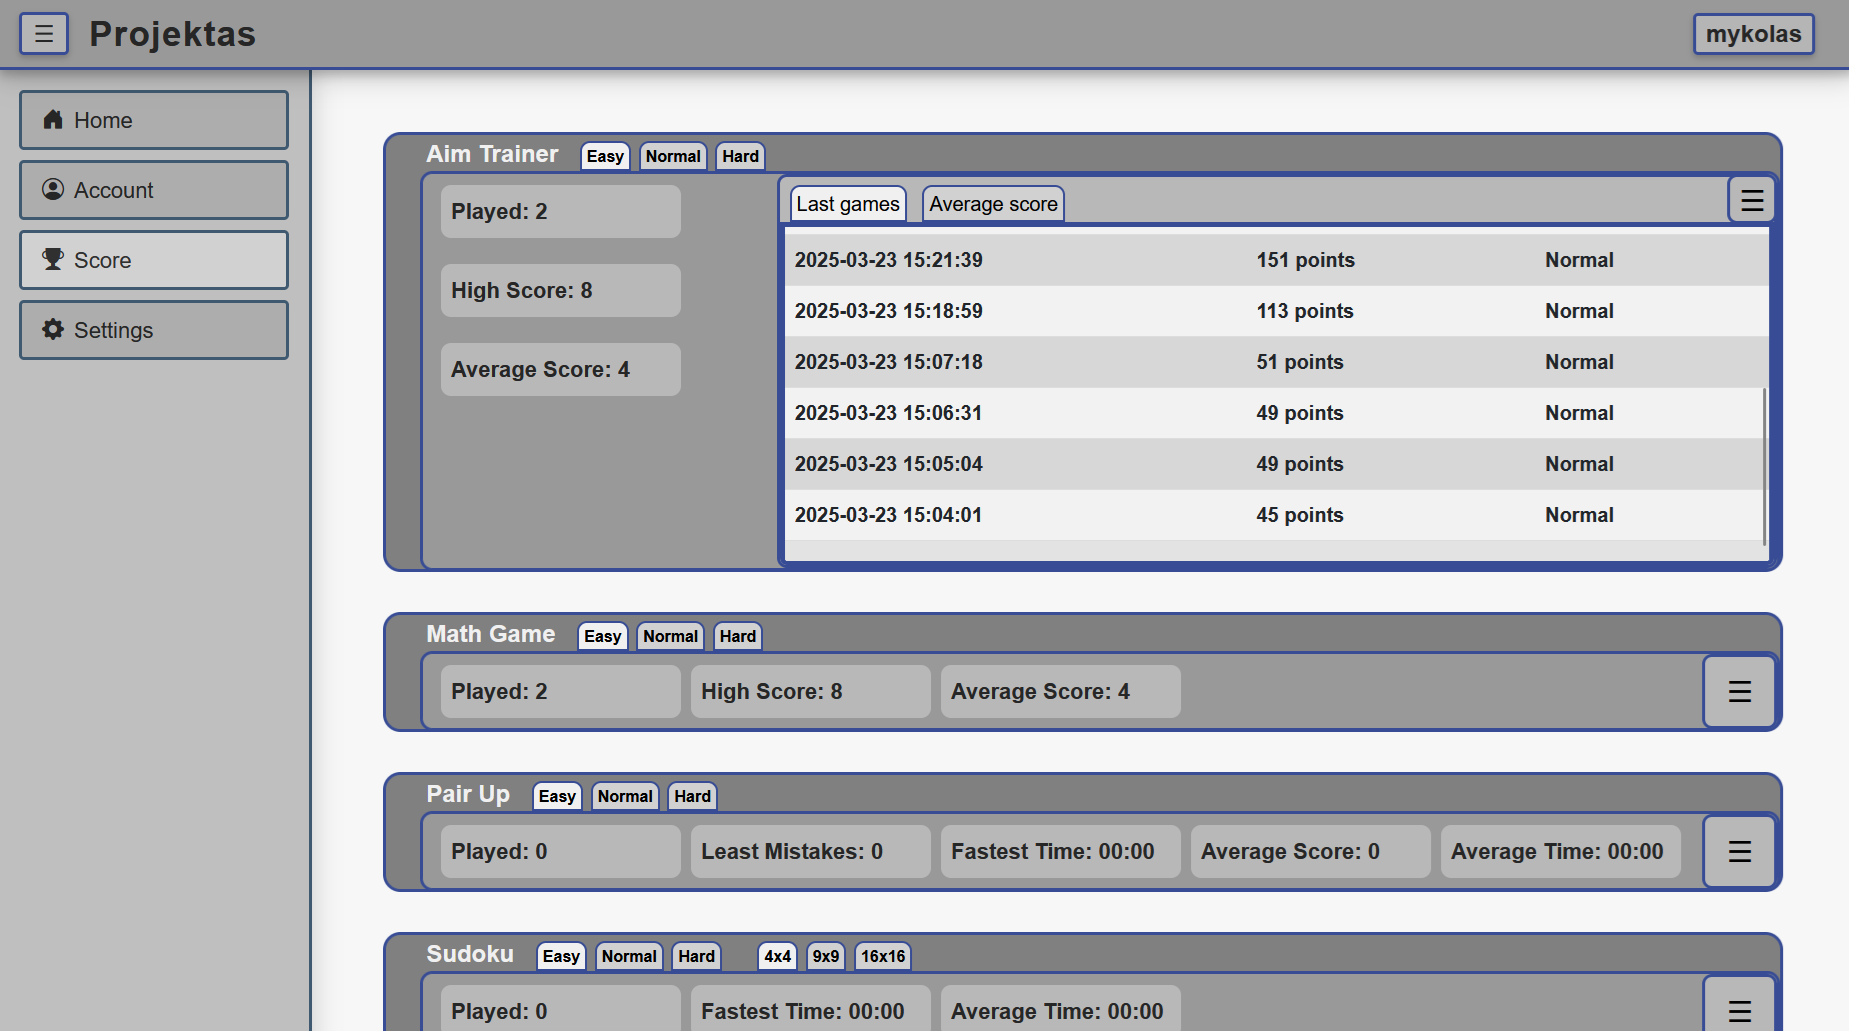
\includegraphics[width=1\textwidth,keepaspectratio]{PSI_3rd_trial/PNGs/timeline_of_played_games.png}
    \caption{Timeline of played games on the score page}
    \label{fig:timeline_of_played_games}
\end{figure}

\begin{figure}[H]
    \centering
    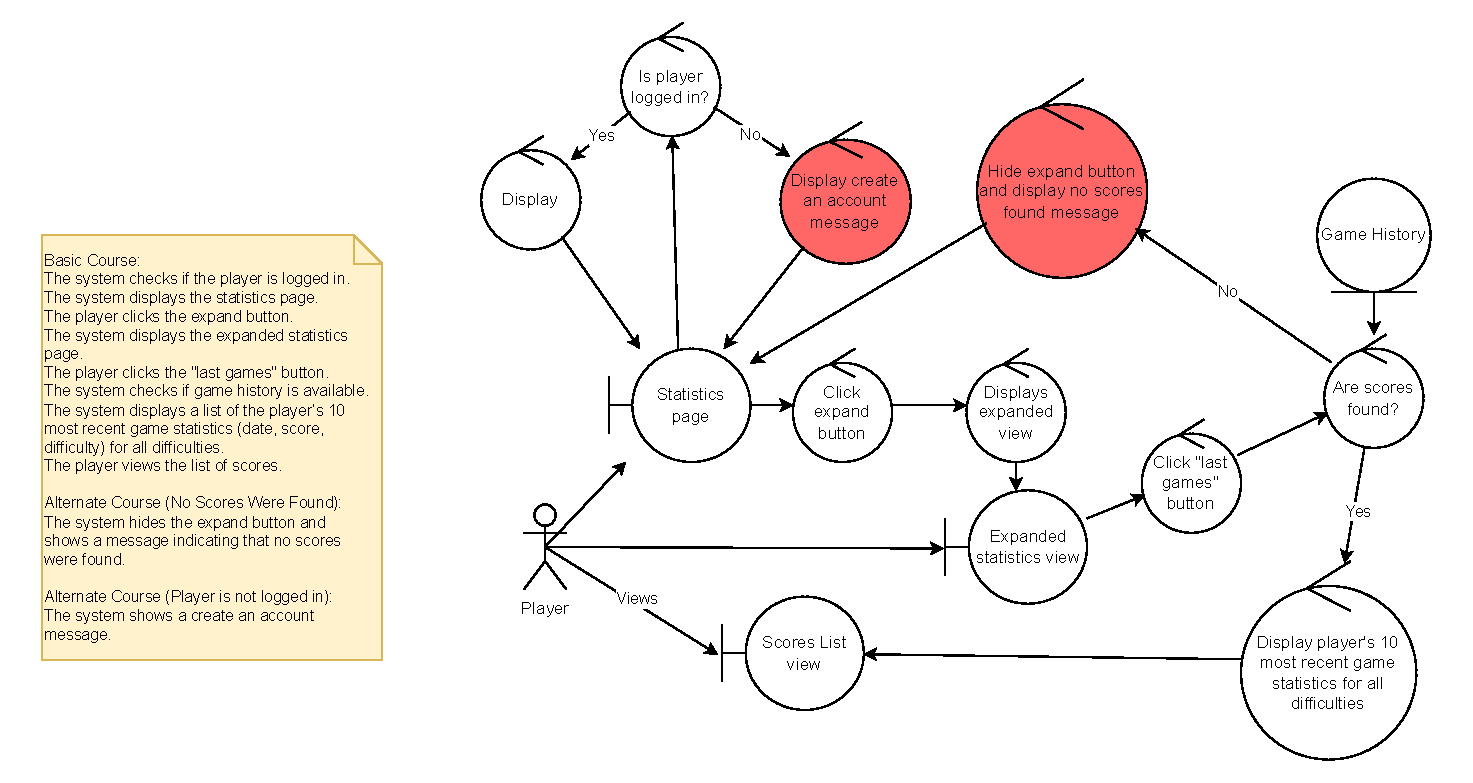
\includegraphics[width=1\textwidth,keepaspectratio]{PSI_3rd_trial/robustness/scores_list.drawio.pdf}
    \caption{View Timeline Of Played Games Robustness Diagram}
    \label{fig:statistics_timeline_view_diagram}
\end{figure}

This use case is derived from the Functional Requirements 1.d, 3.e.

%\lipsum[1-3]



\end{document}
